\documentclass[aspectratio=169]{rosenpass-beamer}

\usepackage[english]{babel}
\usepackage{tikzsymbols}
\usepackage{pgfornament}
\usetikzlibrary{calc}
\usepackage[export]{adjustbox}
\usepackage{minted}
\tcbuselibrary{minted}
\usepackage[autostyle]{csquotes}
\usepackage{dirtytalk}

\makeatletter
 \newenvironment{rustblock}[2][]
    {\VerbatimEnvironment
    \begin{block}{#2}
      \let\FVB@VerbatimOut\minted@FVB@VerbatimOut
      \let\FVE@VerbatimOut\minted@FVE@VerbatimOut
      \minted@configlang{rust}%
      \setkeys{minted@opt@cmd}{fontsize=\small,#1}%
      \minted@fvset
      \begin{VerbatimOut}[codes={\catcode`\^^I=12},firstline,lastline]{\minted@jobname.pyg}}%
    {\end{VerbatimOut}%
        \minted@langlinenoson
        \expandafter\minted@pygmentize\expandafter{\minted@lang}%
        \minted@langlinenosoff%
        \end{block}%
        }
\makeatother

\usetikzlibrary{positioning,decorations.pathreplacing,svg.path}

\definecolor{RPPink}{rgb}{274,4,132}
\definecolor{RPOrange}{rgb}{255, 166, 48}
\definecolor{RPAquamarine}{rgb}{255, 166, 48}
\definecolor{RPLightGray}{rgb}{160, 159, 164}
\definecolor{RPTurquoise}{rgb}{114, 161, 229}

\usepackage{bbding}
\newcommand*\itemtick{\item[\Checkmark]}
\newcommand*\itemfail{\item[\XSolidBrush]}
\newcommand*{\heading}[1]{%
  {
    \hspace*{-0.5cm}#1
    \vspace{1.0em}
  }
}

\title{How to build post-quantum cryptographic protocols and why wall clocks are not to be trusted.}
\subtitle{}
\author{Benjamin Lipp, \textbf{Karolin Varner} \\ \strut \footnotesize with support from Alice Bowman, Marei Peischl, and Lisa Schmidt}
\institute{\url{https://rosenpass.eu}}

\conference{Håck ma's 2024, Schloss in Ottenschlag}
\date{2024-08-29}

\usepackage{biblatex}
\addbibresource{sources.bib}

\graphicspath{{}{graphics/}}

\ExplSyntaxOn
\makeatletter
\tl_new:N \l__ptxcd_rosenpass_interlude_tl
\tl_set_eq:NN \l__ptxcd_rosenpass_interlude_tl \c_novalue_tl
\int_new:N \g__ptxcd_interlude_page_int
\defbeamertemplate{background}{rosenpass-interlude}{
	\exp_args:NV \tl_if_novalue:nTF {\l__ptxcd_rosenpass_interlude_tl} {
		\int_gincr:N \g__ptxcd_interlude_page_int
		\file_if_exist:nF {graphics/rosenpass-interlude-generic-\int_use:N \g__ptxcd_interlude_page_int.jpeg} {
				\file_if_exist:nF {rosenpass-interlude-generic-\int_use:N \g__ptxcd_interlude_page_int.jpeg} {\int_gset:Nn \g__ptxcd_interlude_page_int {1}}
		}
		\includegraphics[width=\paperwidth,height=\paperheight]{rosenpass-interlude-generic-\int_use:N \g__ptxcd_interlude_page_int}
	} {
		\includegraphics[width=\paperwidth,height=\paperheight]{rosenpass-interlude-\l__ptxcd_rosenpass_interlude_tl}
	}
}


\cs_new:cpn {ps@interlude} {%
	\setbeamertemplate{background}[rosenpass-interlude]
	\use:c {ps@navigation}%
}

\setbeamercolor{interlude}{fg=white,bg=}

%\keys_define:nn {ptxcd/rosenpass-interlude}{

\NewDocumentCommand{\interlude}{sD<>{}O{\c_novalue_tl}d<>md<>}{
	\begingroup
		\tl_set:Nn \l__ptxcd_rosenpass_interlude_tl  {#3}
%		\IfNoValueF{#2}{\keys_set:nn {ptxcd/rosenpass-interlude}{#2}}
		\begin{frame}[c]
			\leavevmode
			\thispagestyle{interlude}
			\IfBooleanT{#1}{\setbeamercolor{interlude}{fg=black}}
			\begin{beamercolorbox}[wd=\dimexpr\paperwidth-6ex,sep=3ex,center,#2]{interlude}
				\IfNoValueF{#4}{{\usebeamerfont{interlude-annotation}#4}\par}
				\usebeamerfont{interlude}#5\par
				\IfNoValueF{#6}{{\usebeamerfont{interlude-annotation}#6}\par}
			\end{beamercolorbox}
		\end{frame}
	\endgroup
}

\setbeamerfont{interlude}{size=\Huge}
\setbeamerfont{interlude-annotation}{size=\large}

\newcounter{enumblock}[page]
\ExplSyntaxOff
\newenvironment<>{enumblock}[1]{\renewcommand*{\theenumblock}{\Alph{enumblock}.}\refstepcounter{enumblock}\begin{block}#2{\theenumblock~#1}}{\end{block}}
\newenvironment<>{enumblock*}[1]{\renewcommand*{\theenumblock}{(\arabic{enumblock})}\refstepcounter{enumblock}\begin{block}#2{\theenumblock~#1}}{\end{block}}

\newcommand{\tikzmark}[2][south]{\tikz[overlay,remember picture] \node[anchor=#1] (#2) {\strut};}
\usepackage{transparent}


\AddToHook{env/columns/begin}{%
	\setlength\leftmargini{\labelwidth-\labelsep}% spacing adjustment inside the blocks
 	\setbeamertemplate{block begin}[rosenpass]
}


\RenewDocumentCommand{\blockquote}{o+m}{%
\begingroup%
\arrayrulecolor{rosenpass-blue}\setlength{\arrayrulewidth}{1pt}%
\begin{tabular}{|p{\dimexpr\linewidth-\tabcolsep-\arrayrulewidth}@{}}
#2
\IfNoValueF{#1}{ \tabularnewline\vskip-\parskip\raggedleft#1}
\end{tabular}\par
\endgroup
}

\usepackage{colortbl}

\usepackage{pdfpc}

% test to adjust column spacing
    \defbeamertemplate{block begin}{rosenpass}
    {%
      \begin{beamercolorbox}[colsep*=.75ex]{block title}
        \usebeamerfont*{block title}\insertblocktitle%
      \end{beamercolorbox}%
      {\parskip0pt\par}%
      \ifbeamercolorempty[bg]{block title}
      {}
      {\ifbeamercolorempty[bg]{block body}{}{\nointerlineskip\vskip-0.5pt}}%
      \usebeamerfont{block body}%
      \begin{beamercolorbox}[colsep*=.75ex,vmode]{block body}%
        \ifbeamercolorempty[bg]{block body}{\vskip-.25ex}{\vskip-.75ex}\vbox{}%
    }

\newlength{\defaultframetextheight}
\ExplSyntaxOn
\hook_gput_code:nnn {begindocument/end} {calculate-defaultframetextheight} {
\begingroup
	\def\insertframetitle{\strut}
	\vbox_set:Nn \l_tmpa_box {
		\vbox{}%
		{\parskip0pt\usebeamertemplate***{frametitle}\vskip0.25em}%
	}%
	\dim_gset:Nn \defaultframetextheight {\textheight - \box_ht:N \l_tmpa_box -  \box_dp:N \l_tmpa_box -\ht\strutbox-\dp\strutbox}
\endgroup
}
\newcommand{\stretchcolumn}[1]{
	\vbox_to_ht:nn {\defaultframetextheight} {
		\skip_vertical:n {\c_zero_dim plus .5fil}
		#1
		\skip_vertical:n {\c_zero_dim plus .5fil}
	}
}
\ExplSyntaxOff

\begin{document}

\maketitle

\newcommand*{\citePqwgUrl}{https://eprint.iacr.org/2020/379}
\newcommand*{\citePqwgCode}{PQWG}
\newcommand*{\citePqwg}{\href{\citePqwgUrl}{[\citePqwgCode]}}

\newcommand*{\citeGhpUrl}{https://eprint.iacr.org/2018/024}
\newcommand*{\citeGhpCode}{GHP}
\newcommand*{\citeGhp}{\href{\citeGhpUrl}{[\citeGhpCode]}}

\newcommand*{\citeHpkeUrl}{https://eprint.iacr.org/2020/1499}
\newcommand*{\citeHpkeCode}{HPKE}
\newcommand*{\citeHpke}{\href{\citeHpkeUrl}{[\citeHpkeCode]}}

\newcommand*{\citeXwingUrl}{https://eprint.iacr.org/2024/039}
\newcommand*{\citeXwingCode}{XWING}
\newcommand*{\citeXwing}{\href{\citeXwingUrl}{[\citeXwingCode]}}

\newcommand*{\citeNoiseUrl}{https://noiseprotocol.org/noise.html}
\newcommand*{\citeNoiseCode}{NOISE}
\newcommand*{\citeNoise}{\href{\citeNoiseUrl}{[\citeNoiseCode]}}

\newcommand*{\citeBellareRogawayUrl}{https://eprint.iacr.org/2004/331}
\newcommand*{\citeBellareRogawayCode}{BR06}
\newcommand*{\citeBellareRogaway}{\href{\citeBellareRogawayUrl}{[\citeBellareRogawayCode]}}

\newcommand*{\citeHaleviUrl}{https://eprint.iacr.org/2005/181}
\newcommand*{\citeHaleviCode}{Hal05}
\newcommand*{\citeHalevi}{\href{\citeHaleviUrl}{[\citeHaleviCode]}}

\section{Section: Prelude}

\section{Section Intro}

\begin{frame}[s]{This is the Plan}
  \begin{enumerate}
    \item \textbf{Introducing Rosenpass,} briefly.
    \item \textbf{The Design of Rosenpass} and basics about post-quantum protocols.
    \item \textbf{Hybrid Security} – how it can be done and how we do it.
    \item \textbf{ChronoTrigger Attack} and not trusting wall clocks.
    \item \textbf{Protocol Proofs} – big old rant!
    \item \textbf{Q\&A} – and probably \say{more of a comment}.
  \end{enumerate}

  \begin{center}
    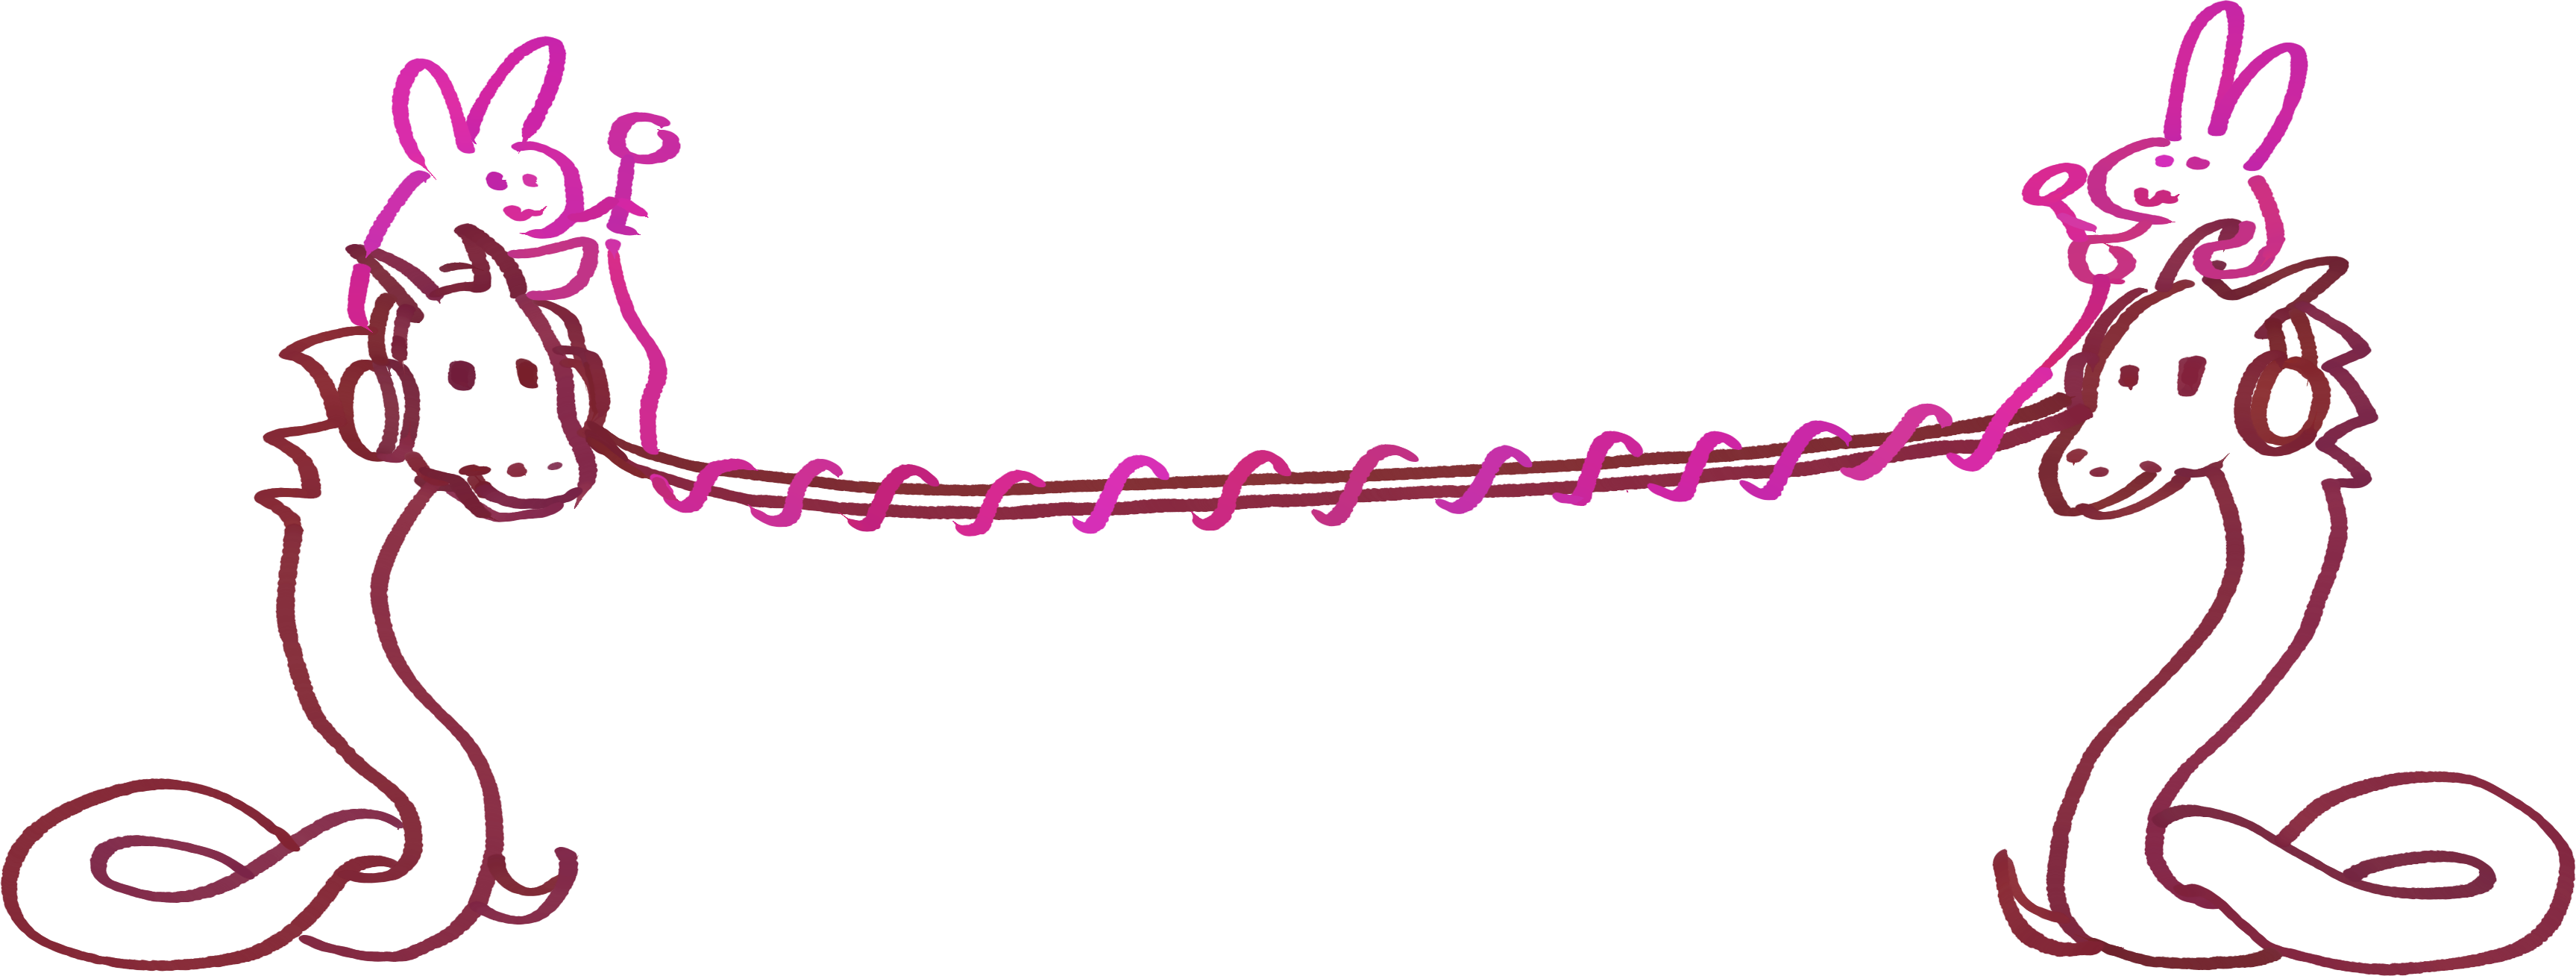
\includegraphics[height=.3\textheight]{graphics/wireguard-and-rp-bunny-rose.png}
  \end{center}
\end{frame}



\begin{frame}{Introducing Rosenpass, briefly}
  \begin{columns}[fullwidth,c]

    \begin{column}{.5\linewidth}
      \begin{itemize}
        \item A post-quantum secure key exchange \textbf{protocol}
          {\small based on the paper Post-Quantum WireGuard~\citePqwg}
        \item An open-source Rust \textbf{implementation} of that protocol, already in use
        \item A way to secure WireGuard VPN setups against quantum attacks
        \item A \textbf{post-quantum secure VPN}
        \item A governance \textbf{organization} to facilitate development, maintenance, and adoption of said protocol
        %\item A translation research organization
      \end{itemize}
      \bigskip
      \textbf{\url{rosenpass.eu}}
    \end{column}%
    \begin{column}{.5\linewidth}
      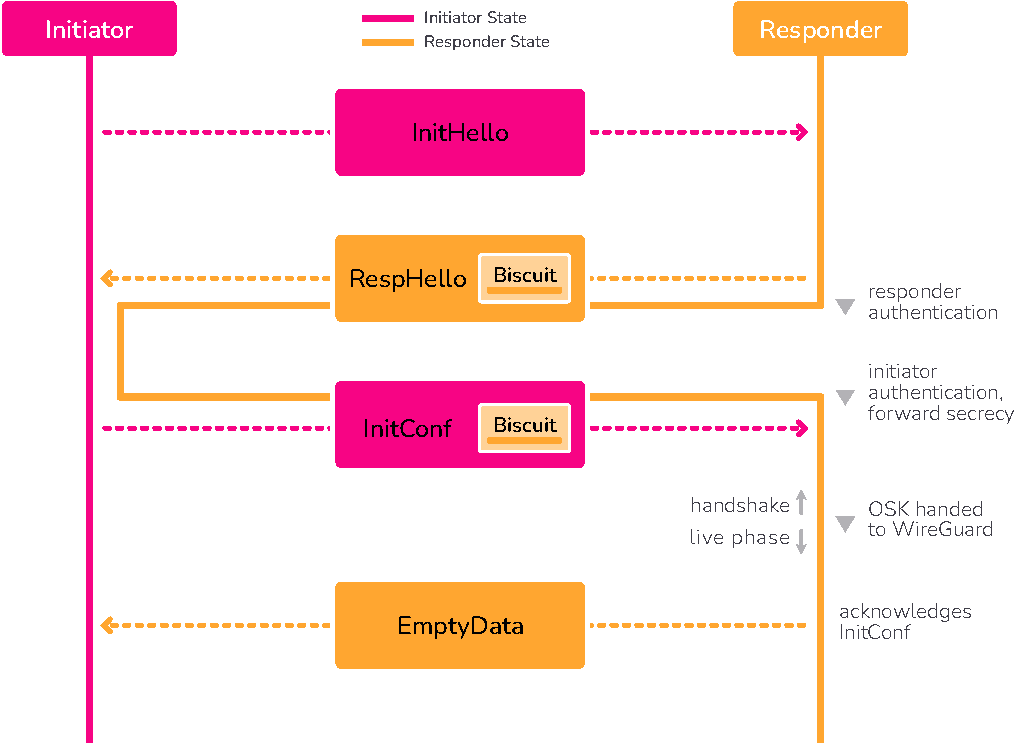
\includegraphics[ width=\linewidth]{graphics/rosenpass-wp-key-exchange-protocol-rgb.pdf}
    \end{column}
  \end{columns}
\end{frame}

\interlude[0]{The design of Rosenpass \\ \vspace{0.8em} \small and how to build post-quantum protocols}
\section{The design of Rosenpass}

\begin{frame}[light]{In the following slides, you will learn…}
  \begin{columns}[c]
    \begin{column}{.40\linewidth}
      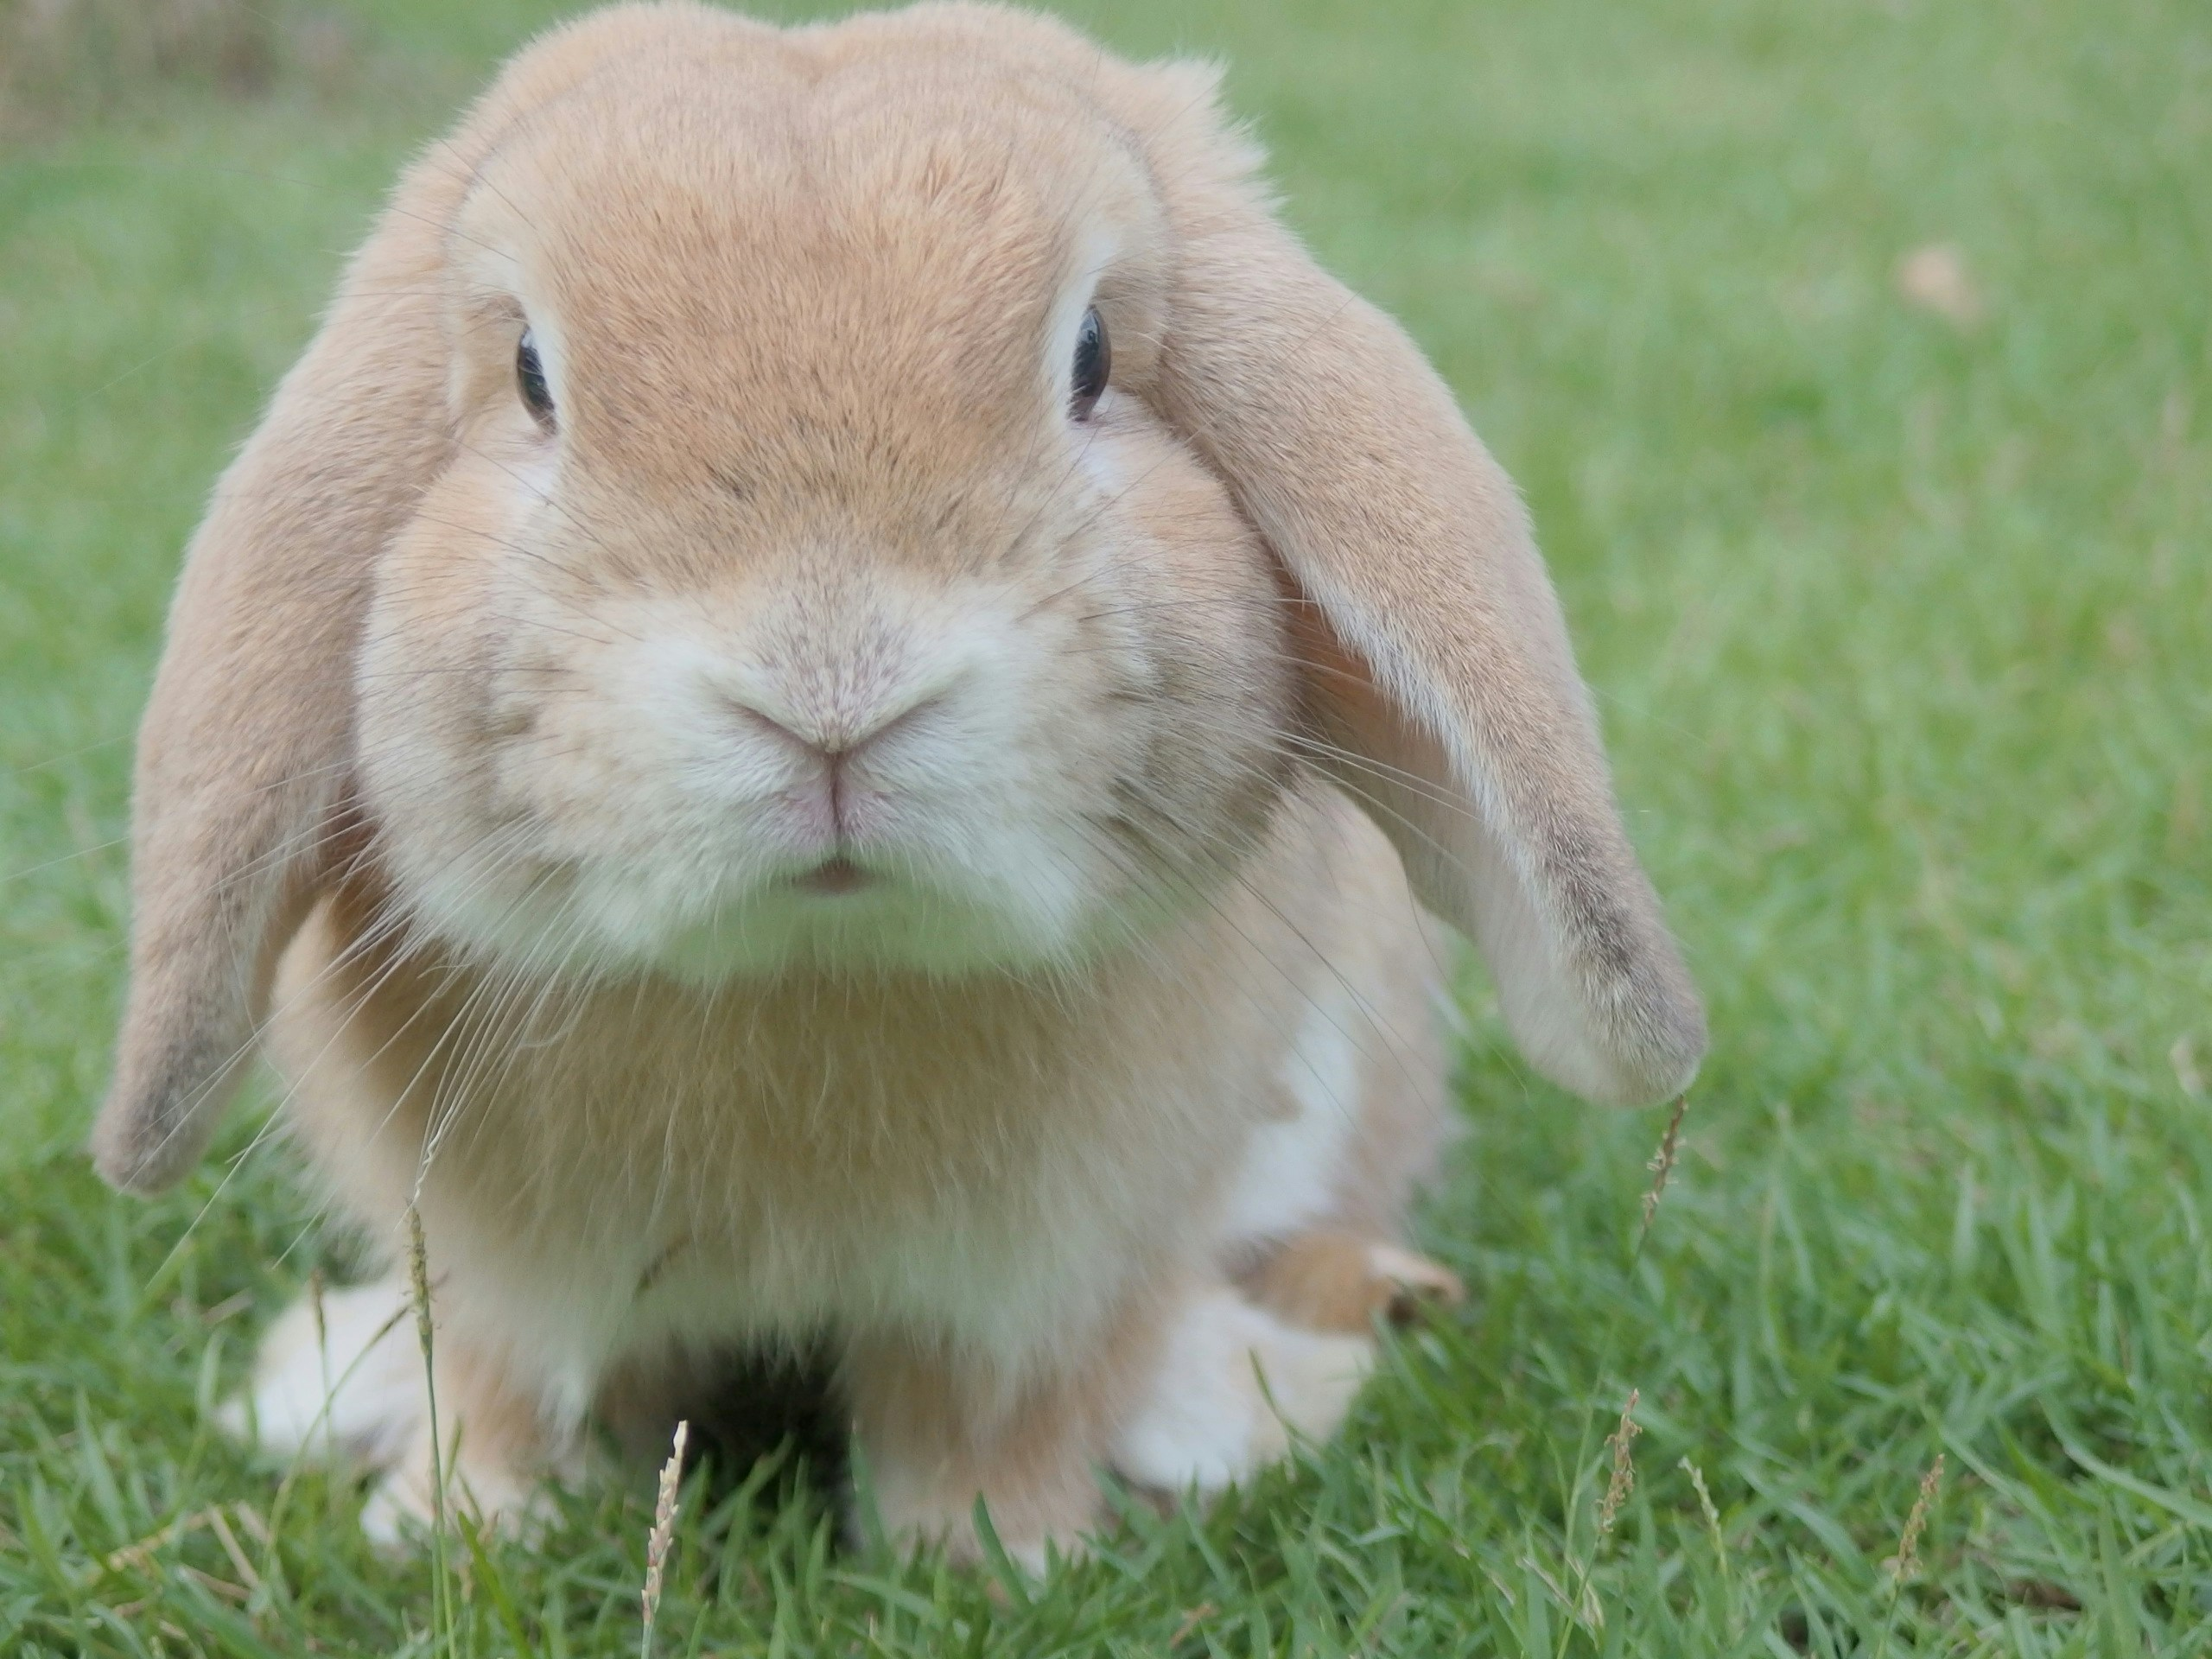
\includegraphics[width=.6\linewidth,right,padding=-.2cm .2cm 0cm .2cm]{graphics/bunny-looking-at-camera.jpg}
      \par
      \includegraphics[width=1.1\linewidth,right]{graphics/coffe-barista-next-to-roaster.jpg}
    \end{column}

    \begin{column}{.60\linewidth}
      …that most cryprographic applications today are susceptible against attacks from quantum computers.

      \vspace{2em}
      …that this is not fundamental to cryptography, but that pre-quantum protocols are simply a more efficient.

      \vspace{2em}
      …that – cryptographically speaking – the difference between pre-quantum and post-quantum crypto is about a subtle
      difference in function interface.
    \end{column}
  \end{columns}
\end{frame}




\begin{frame}{Glossary: Post-quantum security}
\vspace{-\ht\strutbox}
  \begin{columns}[t]
    \begin{column}{.30\linewidth}
      \begin{block}{Pre-quantum Cryptography is… \strut}

      …susceptible to attacks from quantum computers.

      \vspace{0.5em}
      \begin{itemize}
        \item Specifically, to \emph{Shor's Algorithm} % TODO(karolin): Citation needed
        \item Quite fast
        %\item Widely used
        \item Widely widely trusted
      \end{itemize}
      \end{block}
    \end{column}

    \begin{column}{.33\linewidth}
      \begin{block}{Post-quantum cryptography is…}

        …not susceptible to attacks from quantum computers.

      \vspace{0.5em}
      \begin{itemize}
        \item generally less efficient.
        \item much bigger ciphertexts.
        %\item hard to use on embedded devices.
        %\item adoped in the last decade.
        \item less analyzed.
      \end{itemize}
      \end{block}
    \end{column}

    \begin{column}{.36\linewidth}
      \begin{block}{Hybrid cryptography combines…}
        …the combination of the previous two. It is…


        \vspace{0.3em}
        \begin{itemize}
          \item about as inefficient as post-quantum cryptography.
          \item not widely adopted, which is a major problem.
        \end{itemize}
      \end{block}
    \end{column}
  \end{columns}
\end{frame}





\begin{frame}{What post-quantum got}
  \centering
  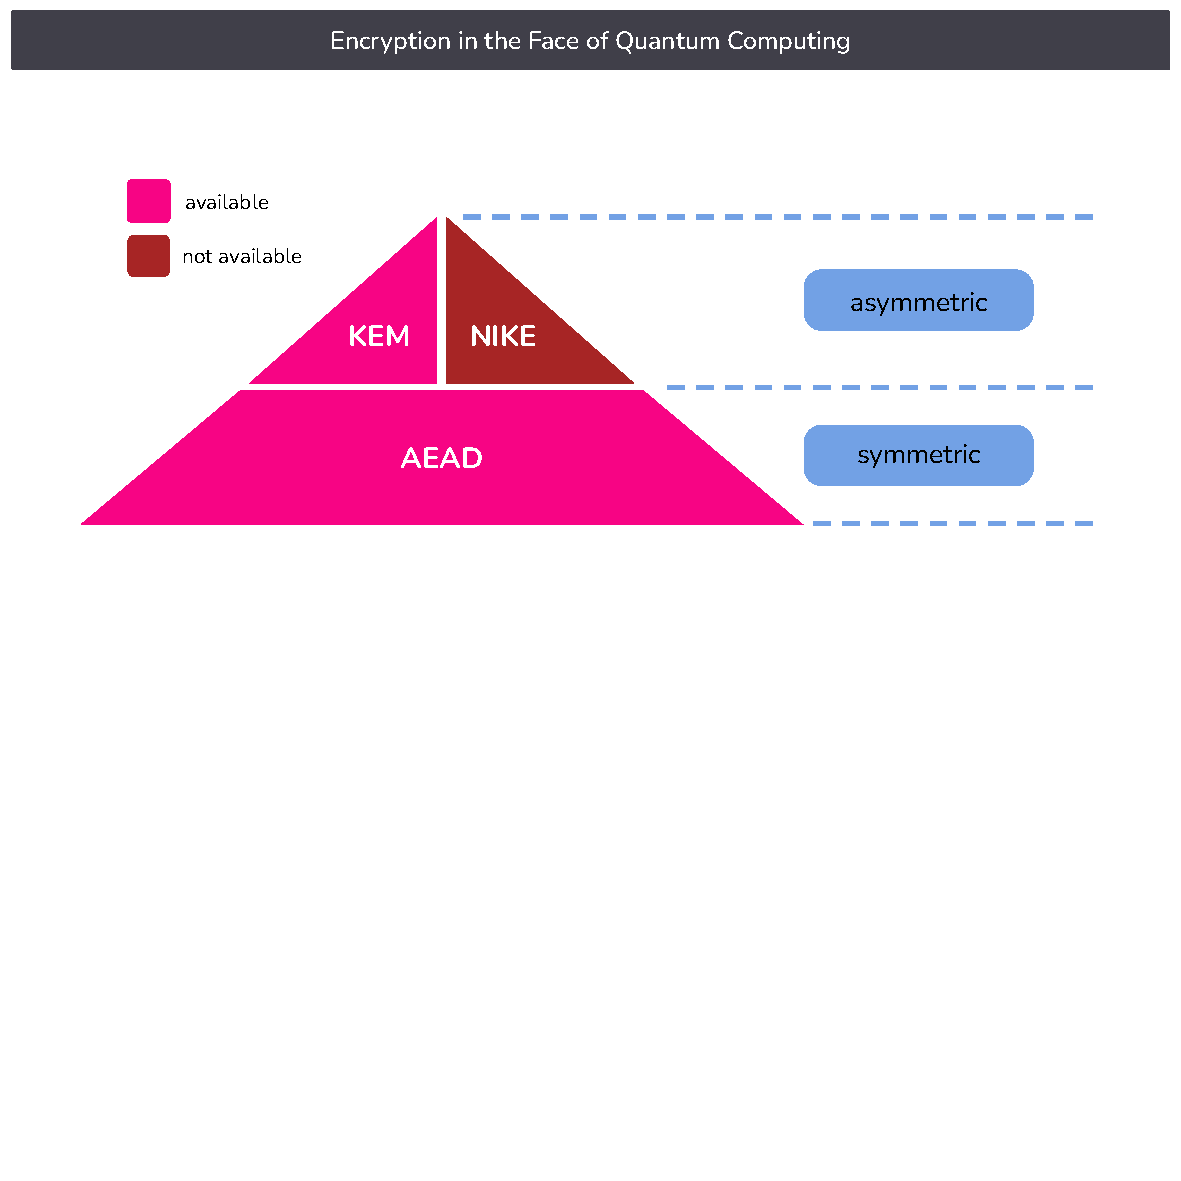
\includegraphics[width=\linewidth,page=1,clip=true,trim=1cm 1cm 0cm 3cm]{graphics/rosenpass-key-exchanges-nike-kem.pdf}
\end{frame}





\begin{frame}[fragile,T]{NIKEs and KEMs}
  \begin{columns}[t,fullwidth]
    \begin{column}{.5\linewidth}
\begin{rustblock}{Key Encapsulation Method}
fn Kem::encaps(Pk) -> (Shk, Ct);
fn Kem::decaps(Pk, Ct) -> Shk;

(shk, ct) = encaps(pk);
assert!(decaps(sk, ct) = shk)
\end{rustblock}
        \vspace{1em}
        Think of it a encrypting a key and sending it
        to the partner.

        \vspace{0.7em}
        \begin{itemize}
          \item Secrecy
          \item Implicit authentication of recipient
            (assuming they have the shared key, they must
            also have their secret key)
        \end{itemize}
    \end{column}%
    \begin{column}{.5\linewidth}
\begin{rustblock}{Non Interactive Key Exchange}
fn nike(sk: Sk, pk: Pk) -> Shk;

assert!(nike(sk1, pk2) = nike(sk2, pk1));
\end{rustblock}

        % TODO(marei): Can you align these using latex instead of empty lines above?
        \vspace{1em}
        Aka. Diffie-Hellman.
        I don't know a good analogy, but ote how the
        keypairs are \emph{crossing over} to each other.

        \vspace{0.7em}
        \begin{itemize}
          \item Secrecy
          \item Mutual authentication
            (for each party: assuming they have the shared key, they must
            also have their secret key)
        \end{itemize}
    \end{column}

  \end{columns}
\end{frame}




\begin{frame}[fragile,t]{NIKEs and KEMs: Key exchange}
  \vspace{-1.5em}
  \begin{columns}[t]
    \begin{column}{.5\linewidth}
      \begin{block}{Key Encapsulation Method}
        % TODO(marei): Can you fix this?
        \begin{description}
          \item[\textbf{Responder Authentication}:] Initiator encapsulates key under the responder public key.
          \item[\textbf{Initiator Authentication}:] Responder encapsulates key under the initiator public key.
          \item[\textbf{Forward-secrecy}:] In case the secret keys get stolen, either party generates a temporary
            and has the other party encapsulate a secret under that keypair.

          \vspace{1em}
          \item[How to do this properly?] See Rosenpass. % TODO: Cite
        \end{description}
      \end{block}
    \end{column}

    \begin{column}{.5\linewidth}
      \begin{block}{Non Interactive Key Exchange}
        \begin{description}[leftmargin=0cm]
          \item[\textbf{Responder Authentication}:] Static-static NIKE since NIKE gives mutual authentication.
          \item[\textbf{Initiator Authentication}:] Static-static NIKE since NIKE gives mutual authentication.
          \item[\textbf{Forward-secrecy}:] Another nike, involving a temporary keypair.

          \vspace{1em}
          \item[How to do this properly?] See the Noise Protocol Framework. % TODO: Cite
        \end{description}
      \end{block}
    \end{column}

  \end{columns}
\end{frame}




\begin{frame}[fragile,T]{NIKEs and KEMs}
  \begin{columns}[t,fullwidth]
    \begin{column}{.5\linewidth}
\begin{rustblock}{Key Encapsulation Method}
trait Kem {
  // Secret, Public, Symmetric, Ciphertext
  type Sk; type Pk; type Shk; type Ct;
  fn genkey() -> (Sk, Pk);
  fn encaps(pk: Pk) -> (Shk, Ct);
  fn decaps(sk: Pk, ct: Ct) -> Shk;
}
#[test]
fn test<K: Kem>() {
  let (sk, pk) = K::genkey();
  let (shk1, ct) = K::encaps(pk);
  let shk2 = K::decaps(sk, ct);
  assert_eq!(shk1, shk2);
}
\end{rustblock}
    \end{column}%
    \begin{column}{.5\linewidth}
\begin{rustblock}{Non Interactive Key Exchange}
trait Nike {
  // Secret, Public, Symmetric
  type Sk; type Pk; type Shk;
  fn genkey() -> (Sk, Pk);
  fn nike(sk: Sk, pk: Pk) -> Shk;
}
#[test]
fn test<N: Nike>() {
  let (sk1, pk1) = N::genkey();
  let (sk2, pk2) = N::genkey();
  let ct1 = N::nike(sk1, pk2);
  let ct2 = N::nike(sk2, pk1);
  assert_eq!(ct1, ct2);
}
\end{rustblock}
    \end{column}

  \end{columns}
\end{frame}




\begin{frame}{Rosenpass Kex Exchange Parts}
  \centering
  \includegraphics[width=.9\linewidth,page=6,clip=true,trim=1cm 4cm 0cm 2cm]{graphics/rosenpass-key-exchanges-nike-kem.pdf}
\end{frame}




% \begin{frame}{Rosenpass Unified Key Exchange}
%   \centering
%   \begin{columns}[fullwidth,c]
%     \begin{column}{.6\linewidth}
%       \includegraphics[width=1.3\linewidth,page=7,clip=true,trim=1cm 4cm 0cm 2cm]{graphics/rosenpass-key-exchanges-nike-kem.pdf}
%     \end{column}%

%     \begin{column}{.4\linewidth}
%       \includegraphics[width=\linewidth,page=5,clip=true,trim=3cm 7cm 0cm 3.5cm]{graphics/rosenpass-key-exchanges-nike-kem.pdf}
%     \end{column}
%   \end{columns}
% \end{frame}





\begin{frame}{Rosenpass Protocol Features}
  \begin{columns}[fullwidth,c]
    \begin{column}{.6\linewidth}
      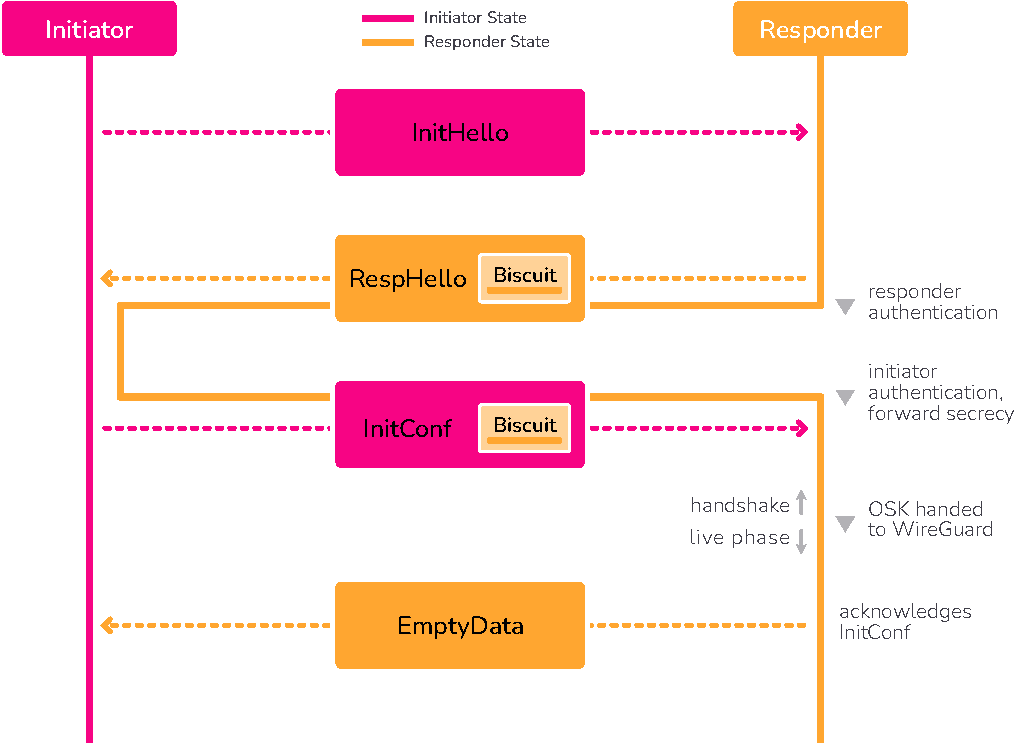
\includegraphics[width=\linewidth]{graphics/rosenpass-wp-key-exchange-protocol-rgb.pdf}
    \end{column}

    \begin{column}{.4\linewidth}
      \begin{itemize}
        \item Authenticated key exchange
        \item Three KEM operations interleaved to achieve mutual authentication and forward secrecy
        \item No use of signatures
        \item First package (InitHello) is unauthenticated
        \item Stateless responder to avoid disruption attacks
      \end{itemize}
    \end{column}
  \end{columns}
\end{frame}

\interlude[1]{Hybridization}
\begin{frame}[light,s]{}
  \vspace{1cm}
  \large
  \vollkorn

  \begin{columns}[c]
    \begin{column}{.30\linewidth}
      % \vfill
      %  …that hybrid, practical, post-quantum cryptography is built by combining pre-quantum and post-quantum primitives.

      % \vfill
      %  …that key encapsulation methods can be combined, rendering a protocol like Rosenpass useful in pre-quantum as well
      %  as post-quantum settings.

      %  \vfill
      %  …why combining protocols like WireGuard and Rosenpass directly is still useful to enable code-reuse and to avoid
      %  loosing trust in established systems like WireGuard.
      %  \vfill
      In the following slides you will learn …
      \par\vspace{1.5em}
      … that hybrid security can be achieved by building hybrid primitives and that it is not always wise to do so.
    \end{column}

    \begin{column}{.40\linewidth}
      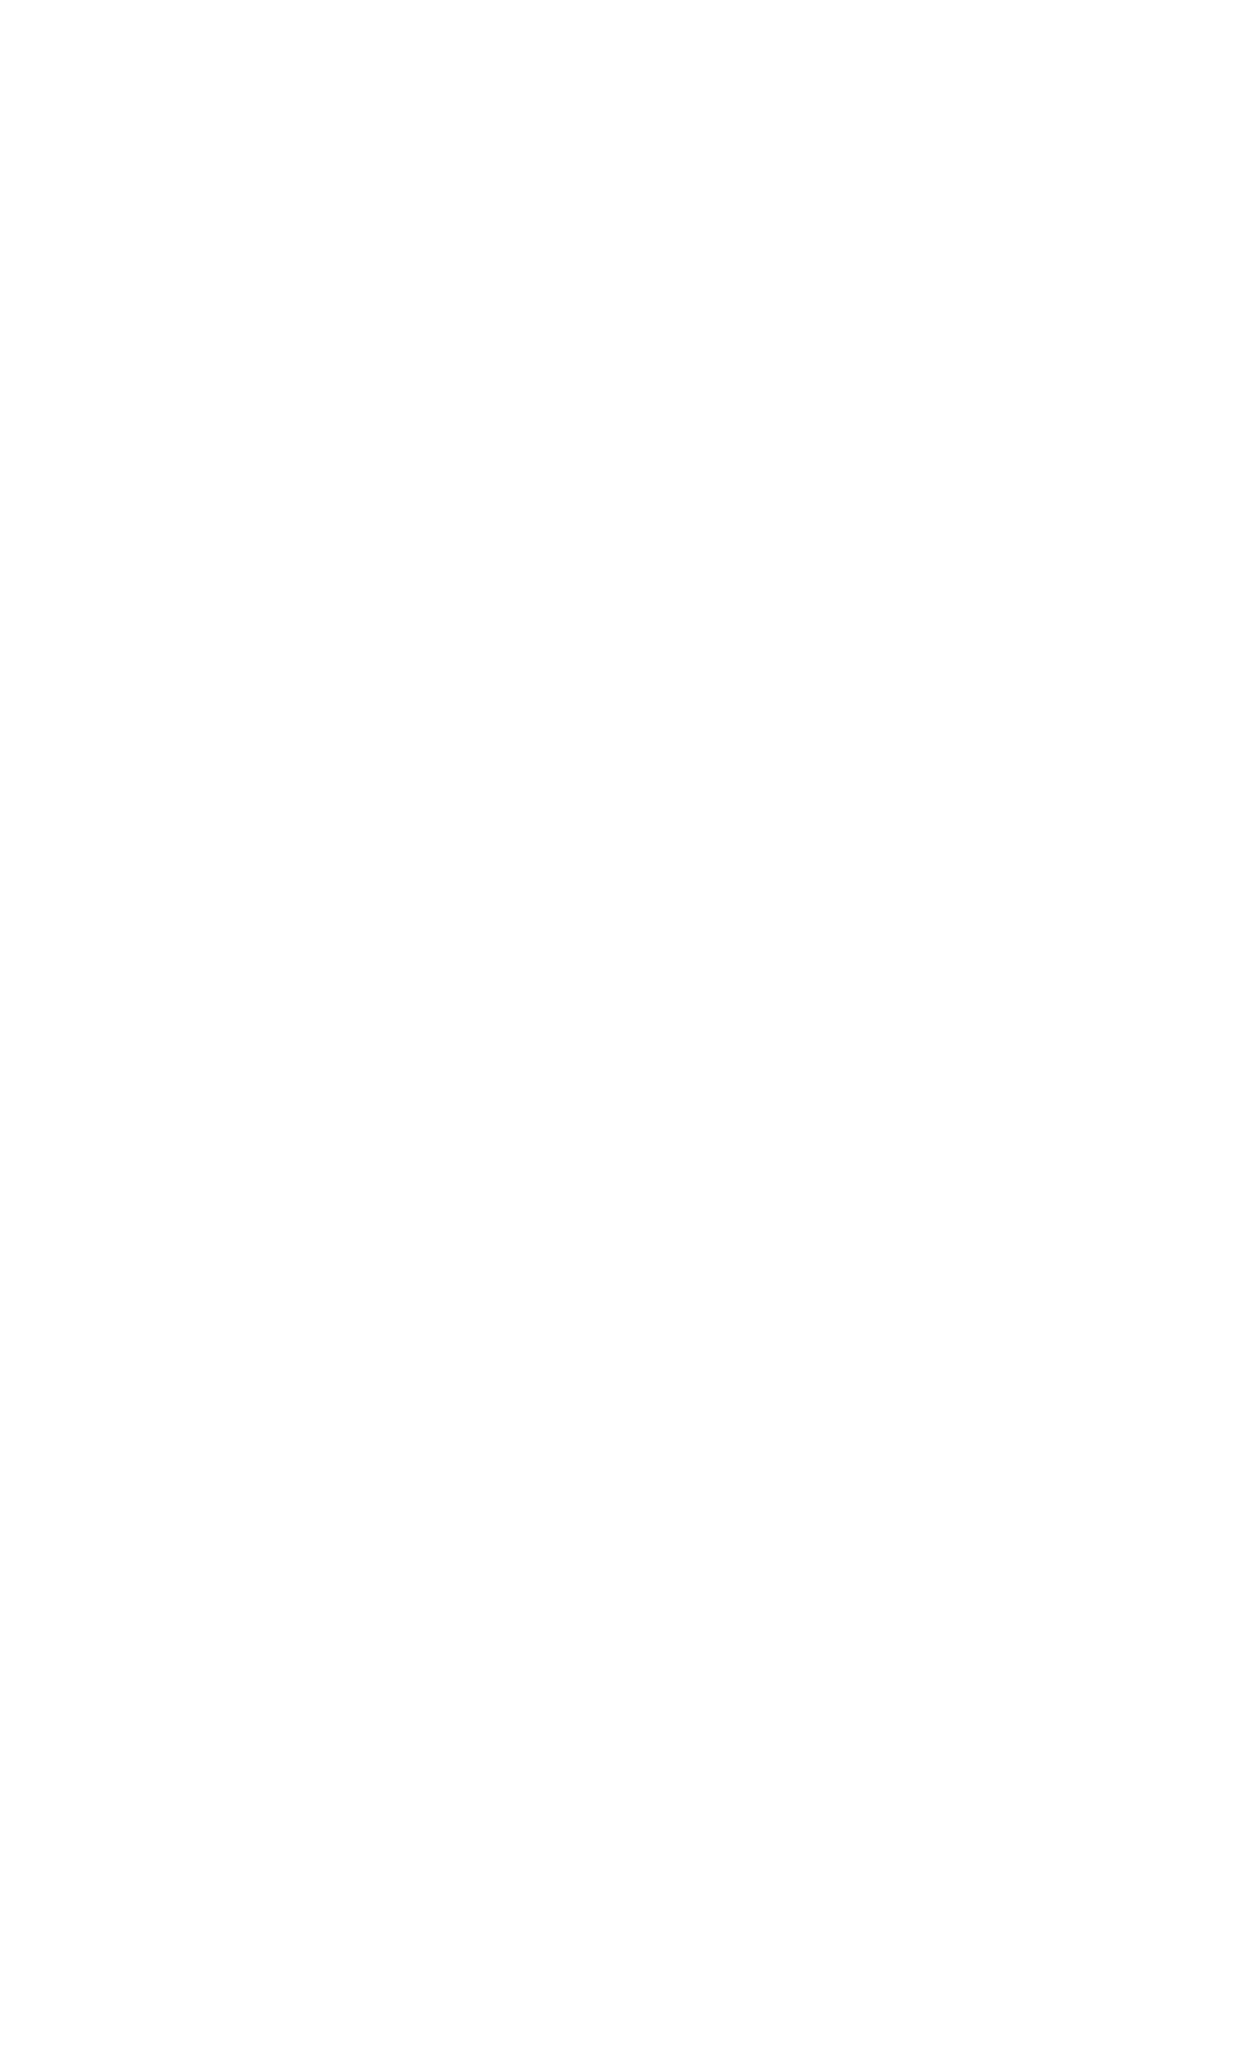
\includegraphics[width=.7\linewidth,padding=-.2cm .2cm .2cm .2cm]{graphics/krapfen-prezel-bunny.pdf}
    \end{column}
  \end{columns}
\end{frame}

\begin{frame}{Combining two KEMs with the GHP Combiner}
  \begin{columns}[c]
    \begin{column}{.4\linewidth}
      \small
      \begin{itemize}
        \item \say{Giacon-Heuer-Poettering} \citeGhp
        \item running both KEMs in parallel
        \item secret keys, public keys, and ciphertexts are concatenated
        \item shared keys are hashed together
        \item ciphertexts included in hash for proof-related reasons
      \end{itemize}
    \end{column}
    \begin{column}{.55\linewidth}
     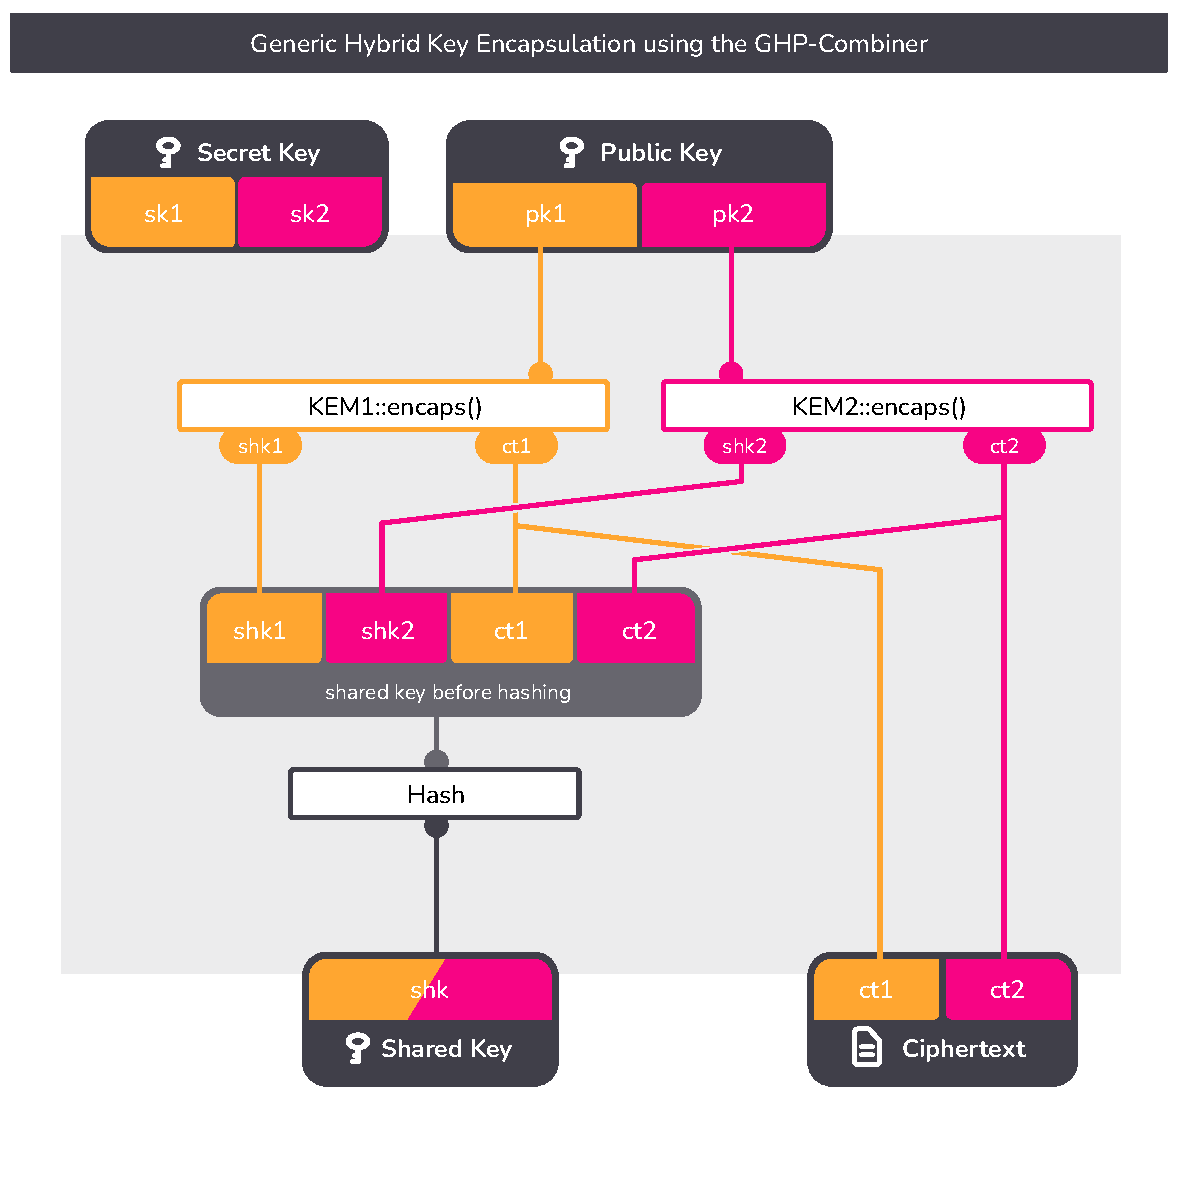
\includegraphics[width=\linewidth,page=1,clip=true,trim={29 43  29 58}]{graphics/rosenpass-encapsulation-combiner.pdf}
    \end{column}
  \end{columns}
\end{frame}


\begin{frame}{Turning a NIKE into a KEM}
  \begin{columns}[c]
    \begin{column}{.55\linewidth}
    \includegraphics[width=\linewidth,page=2,clip=true,trim={29 43  29 58}]{graphics/rosenpass-encapsulation-combiner.pdf}
    \end{column}%
    \begin{column}{.45\linewidth}
      \small
      \begin{itemize}
        \item from the HPKE RFC \citeHpke
        \item \emph{remote} keypair is static keypair
        \item \emph{local} keypair is temporary keypair
        \item local keypair public key is treated as ciphertext
        \item for proof-related reasons, ciphertext and public key
          are included in hash
        \item work by Blanchet, Hauck, Kiltz, Lipp, Riepel
      \end{itemize}
    \end{column}
  \end{columns}
\end{frame}

\begin{frame}{X-Wing \citeXwing}
  \begin{columns}[c]
    \begin{column}{.4\linewidth}
      \small
      \begin{itemize}
        \item combines ML-KEM and x25519
        \item techniques from DHKEM to turn x25519 into a KEM
        \item techniques from GHP to combine the two
        \item optimizations applied to make hashing more efficient
        \item bespoke proof of security
        \item work by Borbosa, Connolly, Duarte, Schwabe, Varner, Westerbaan
      \end{itemize}
    \end{column}
    \begin{column}{.55\linewidth}
      \includegraphics[width=\linewidth,page=3,clip=true,trim={29 43  29 58}]{graphics/rosenpass-encapsulation-combiner.pdf}
    \end{column}

  \end{columns}
\end{frame}

\begin{frame}{Rosenpass \& WireGuard Hybridization}
  \begin{columns}[c]
    \begin{column}{.5\linewidth}
      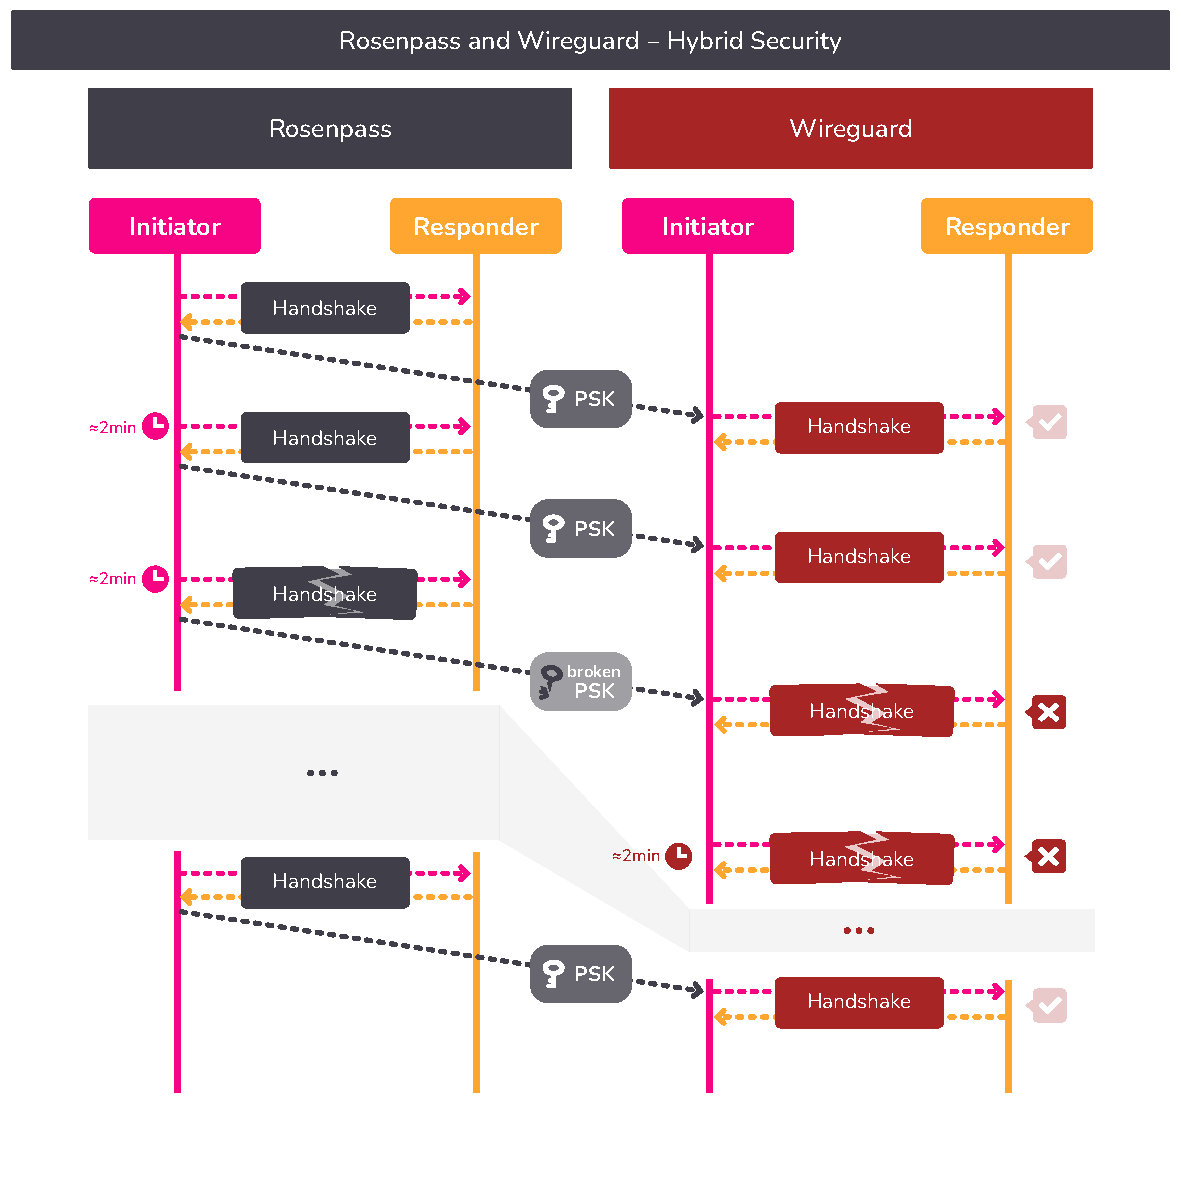
\includegraphics[width=\linewidth, clip=true,trim=42 41 42 42]{graphics/rosenpass-wireguard-hybrid-security.pdf}
    \end{column}
    \begin{column}{.45\linewidth}
      \small
      \begin{itemize}
        \item Rosenpass and WireGuard are hybridized on the procol level
        \item preserving efficiency of and trust in WireGuard
        \item straightforward transition path; existing WireGuard implementation remains in use
        \item key from Rosenpass used as PSK in WireGuard
      \end{itemize}
    \end{column}

  \end{columns}
\end{frame}

\begin{frame}{Full Protocol Reference in the Whitepaper}
  \begin{columns}[c,fullwidth]

    \begin{column}{.65\linewidth}
      \only<1>{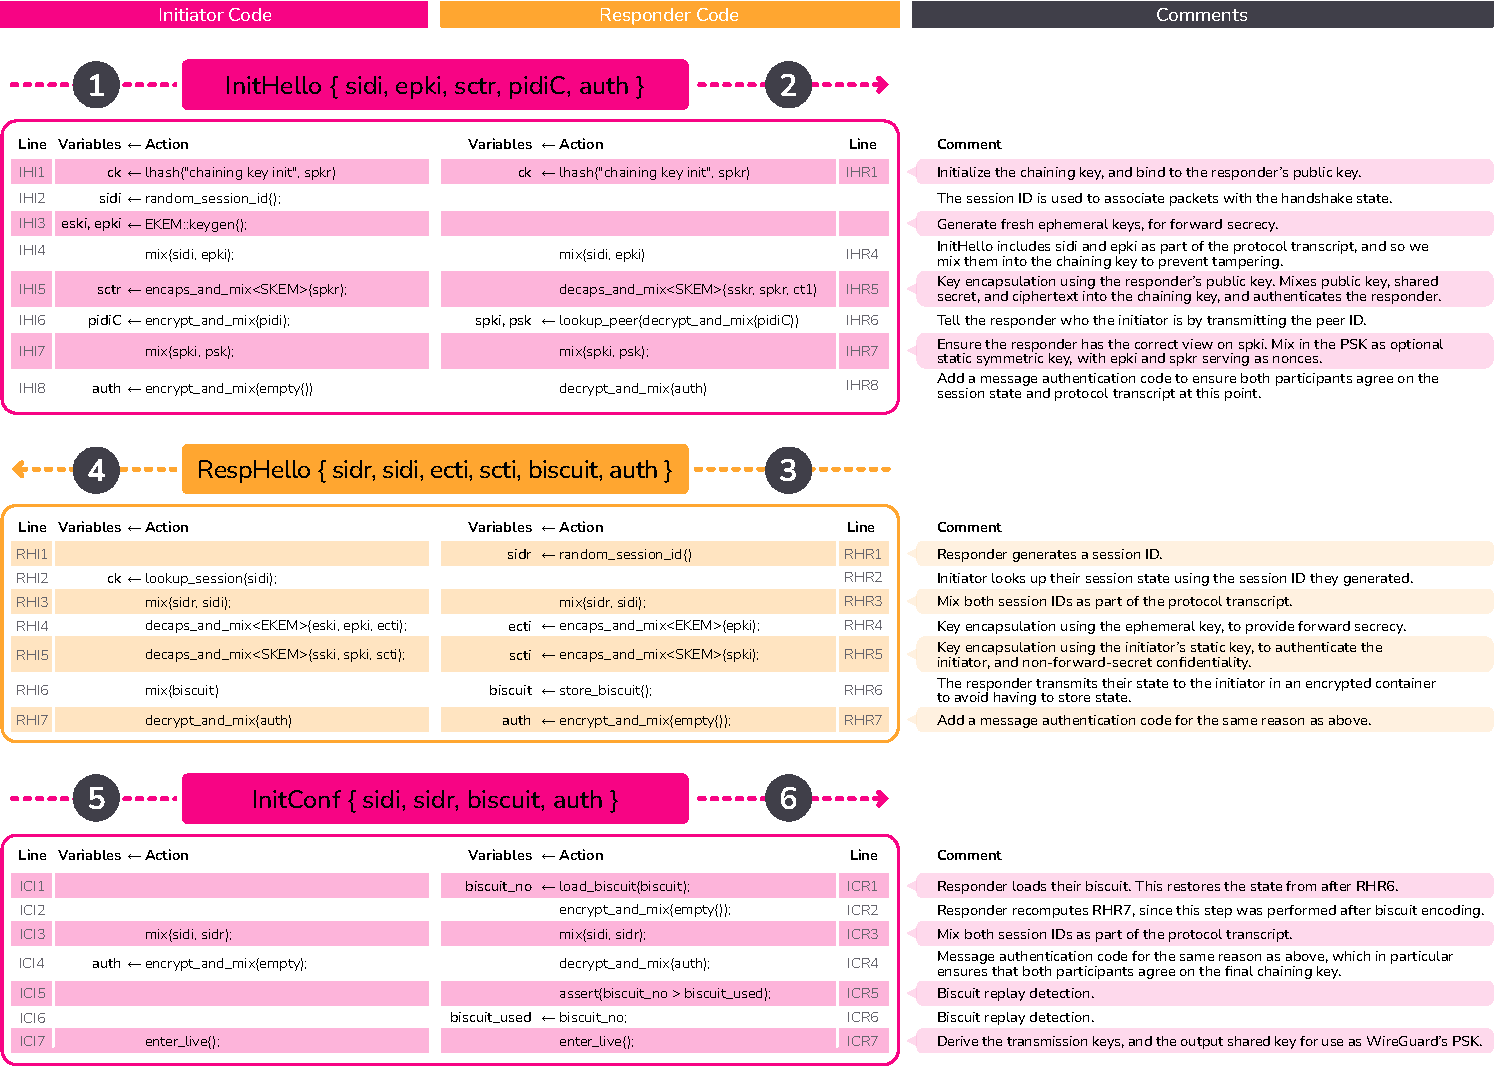
\includegraphics[height=.91\textheight]{graphics/rosenpass-wp-message-handling-code-rgb.pdf}}
      \only<2>{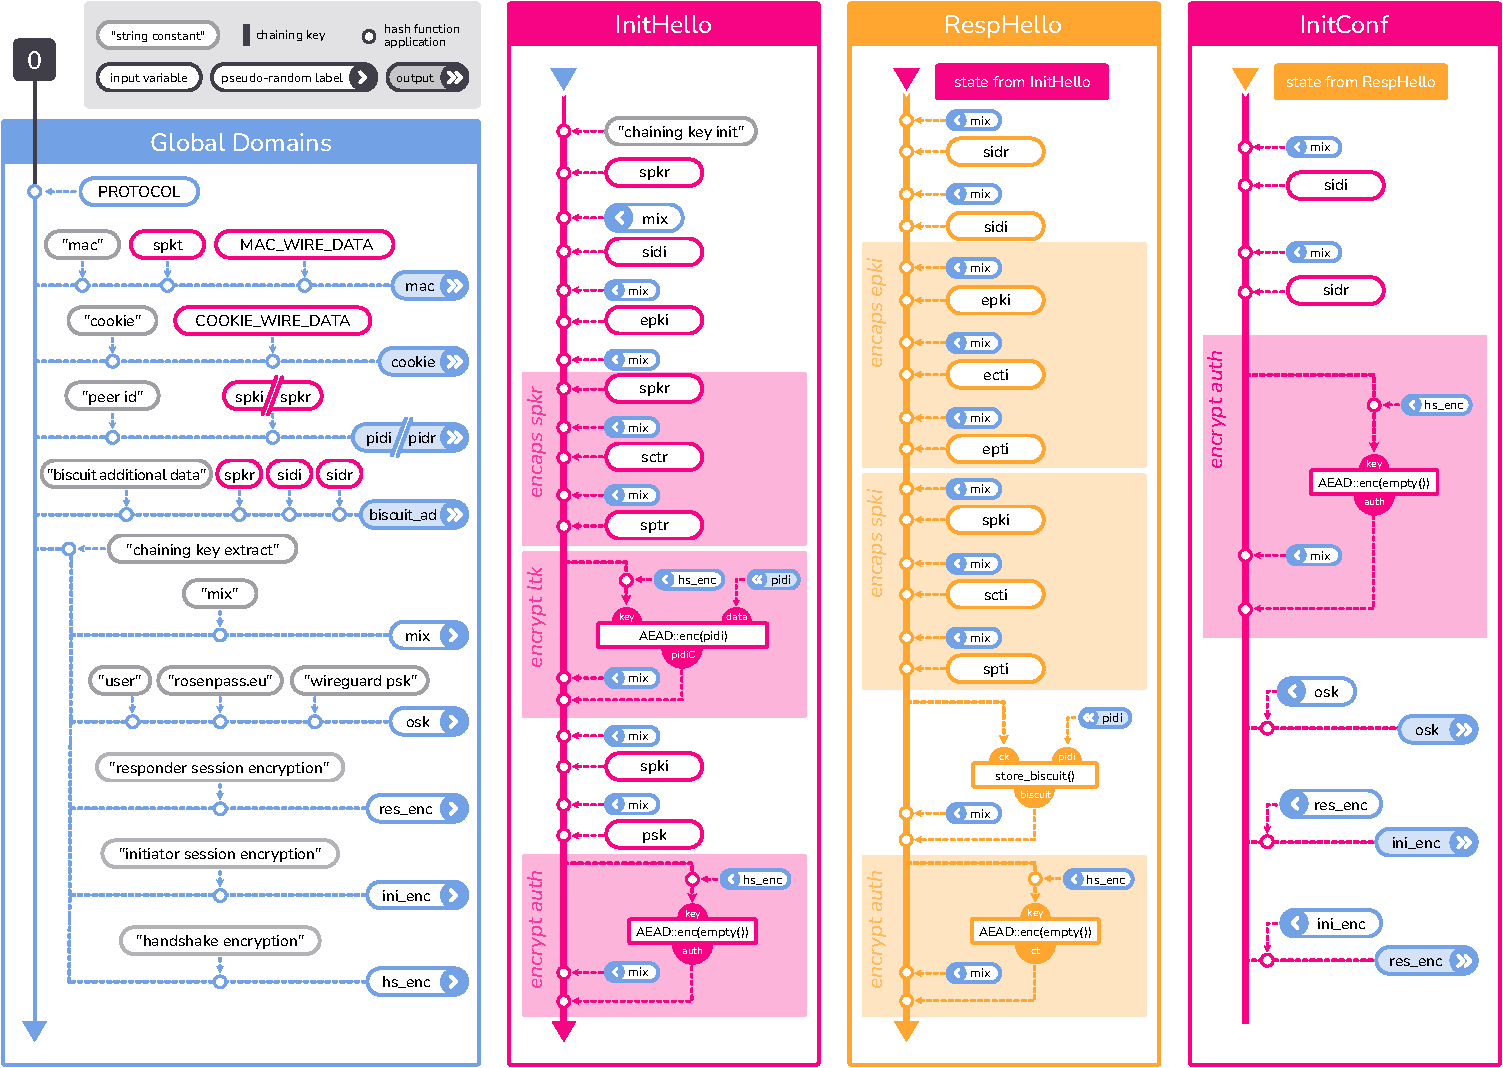
\includegraphics[height=.91\textheight]{graphics/rosenpass-wp-hashing-tree-rgb.pdf}}
    \end{column}

    \begin{column}{.35\linewidth}

      \qrcode[height=1.2cm]{https://rosenpass.eu/docs}
      \\ \url{rosenpass.eu/docs}

      \vspace{1em}
      \qrcode[height=1.2cm]{https://rosenpass.eu/whitepaper.pdf}
      \\ \url{rosenpass.eu/whitepaper.pdf}
    \end{column}

  \end{columns}
\end{frame}

\interlude[2]<Trials \textasciitilde\ Attacks found>{ChronoTrigger}
\hypertarget{state-disruption}{%
\section{State Disruption}\label{state-disruption}}

\begin{frame}{In the following slides, you will learn…}
\hypertarget{you-will-learn-hybrid}{}
\begin{columns}[fullwidth]
  \begin{column}{.58\linewidth}
    …that denial of service can happen on the level of cryptography protocols!

    \vspace{2em}
    …that the wall clock is not to be trusted.

    \vspace{2em}
    …how to accept replay attacks and face them without fear!
  \end{column}
  \begin{column}{.20\linewidth}
    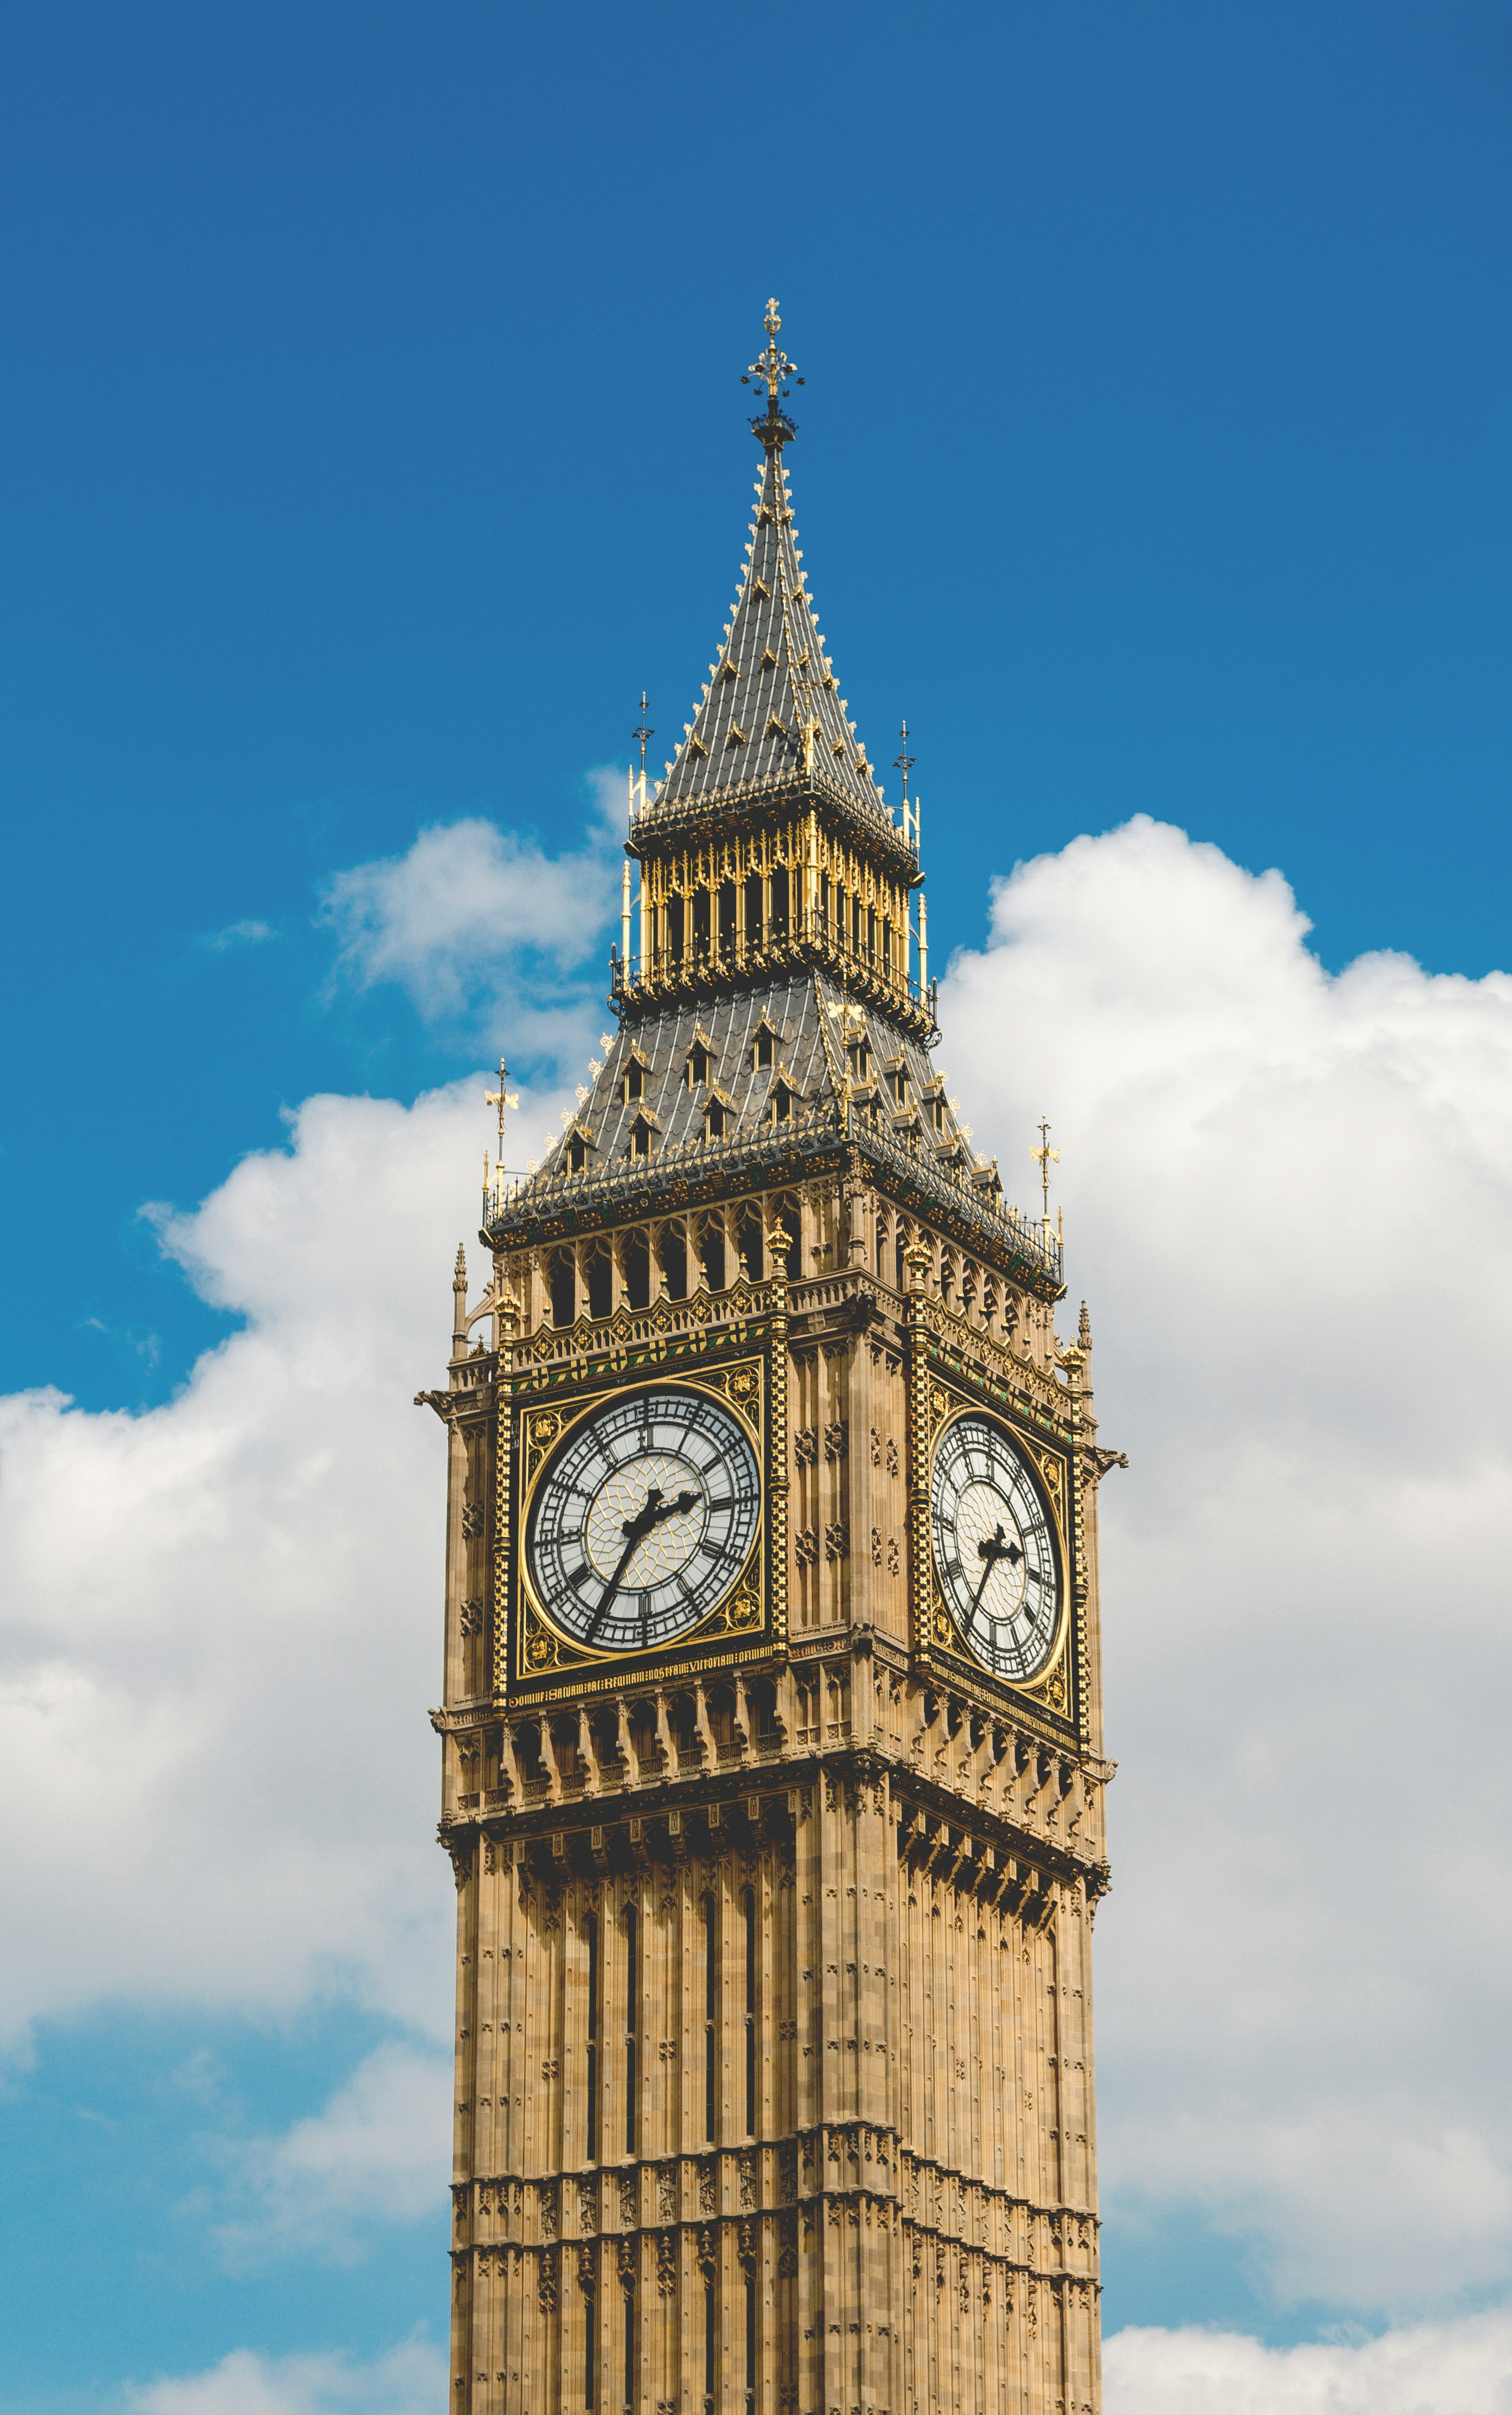
\includegraphics[width=\linewidth]{graphics/big-ben.jpg}
    \vspace{0.4cm}
  \end{column}
  \begin{column}{.20\linewidth}
    \vspace{1.6cm}
    \includegraphics[width=\linewidth]{graphics/sad-bunny-looking-left.jpg}
  \end{column}
\end{columns}
\end{frame}


\begin{frame}{What are State Disruption Attacks?}
  \raisebox{0pt}[0pt][0pt]{
    \begin{minipage}{\textwidth}
      \vspace{2.2cm}
      \begin{columns}[T,fullwidth]
        \begin{column}{.325\linewidth}
          \reflectbox{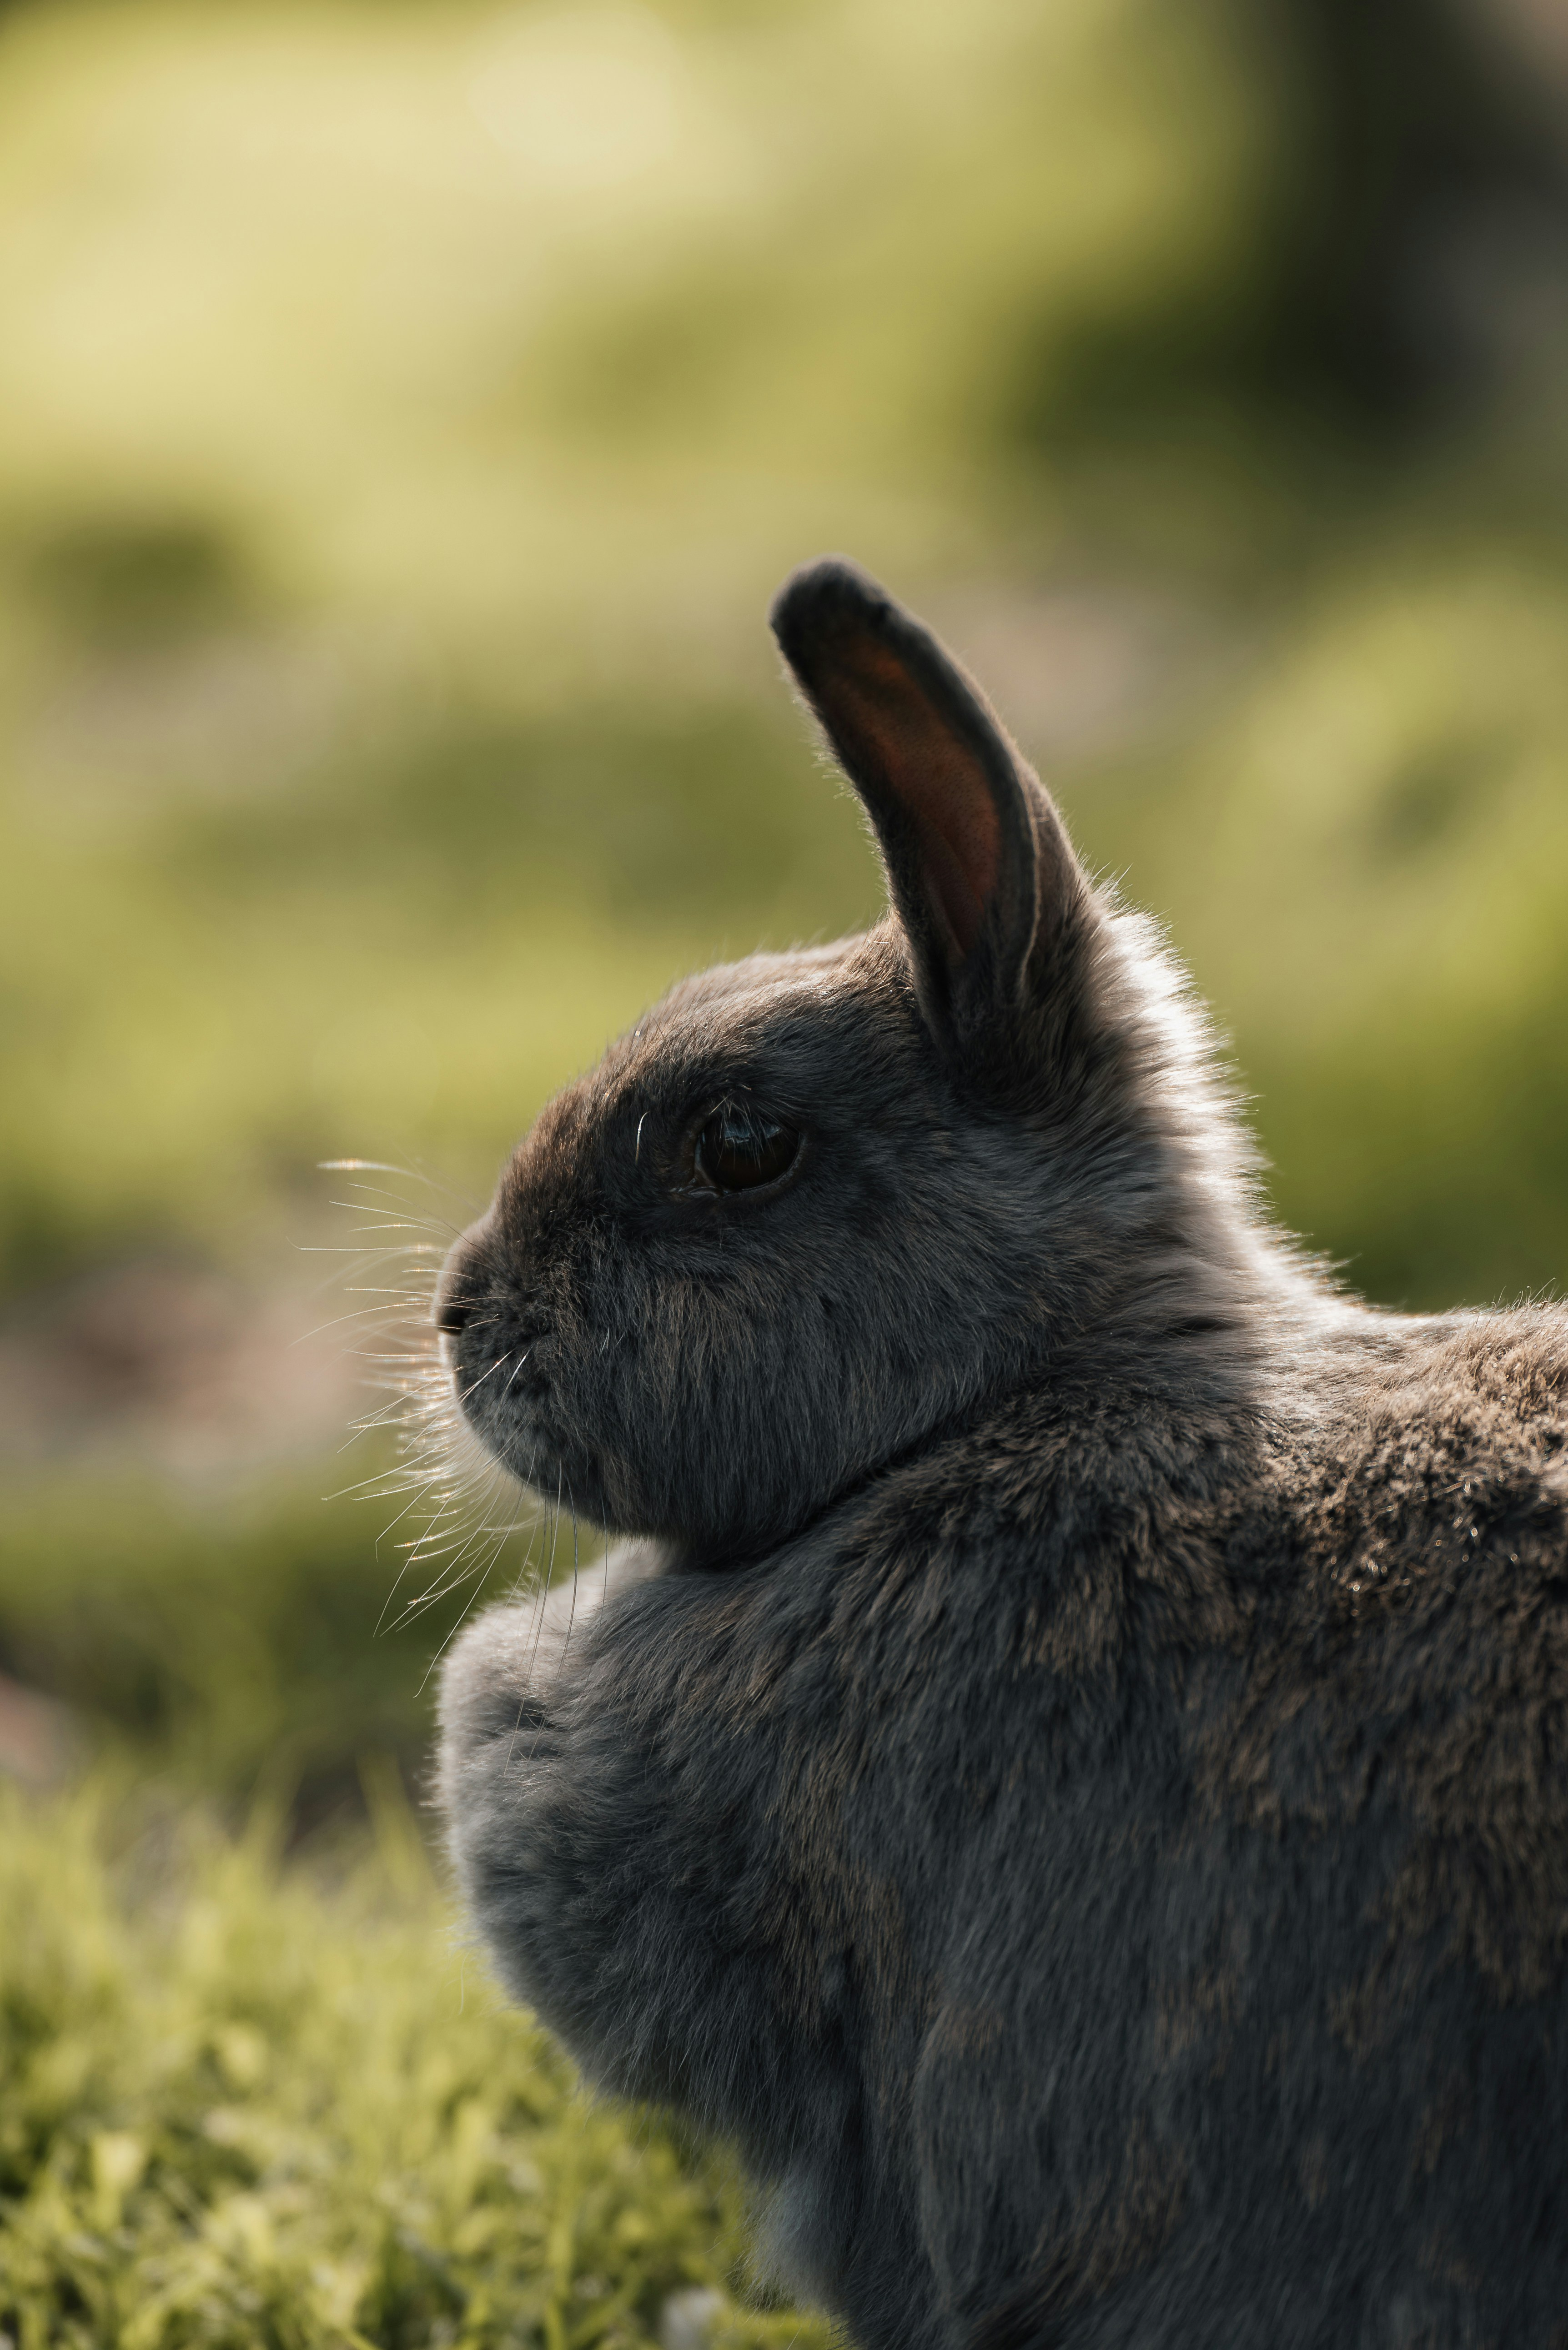
\includegraphics[width=0.9\linewidth,height=.454\textheight,padding=0cm 0cm .5cm 3cm,right,clip,trim={0cm 16cm 0cm 40cm}]{graphics/bunny-2.jpg}}
        \end{column}
        \begin{column}{.35\linewidth}
          \centering
          \includegraphics[width=0.9\linewidth,height=.85\textheight,trim={7cm 38cm 5cm 10cm},clip]{graphics/wires.jpg}
        \end{column}
        \begin{column}{.325\linewidth}
          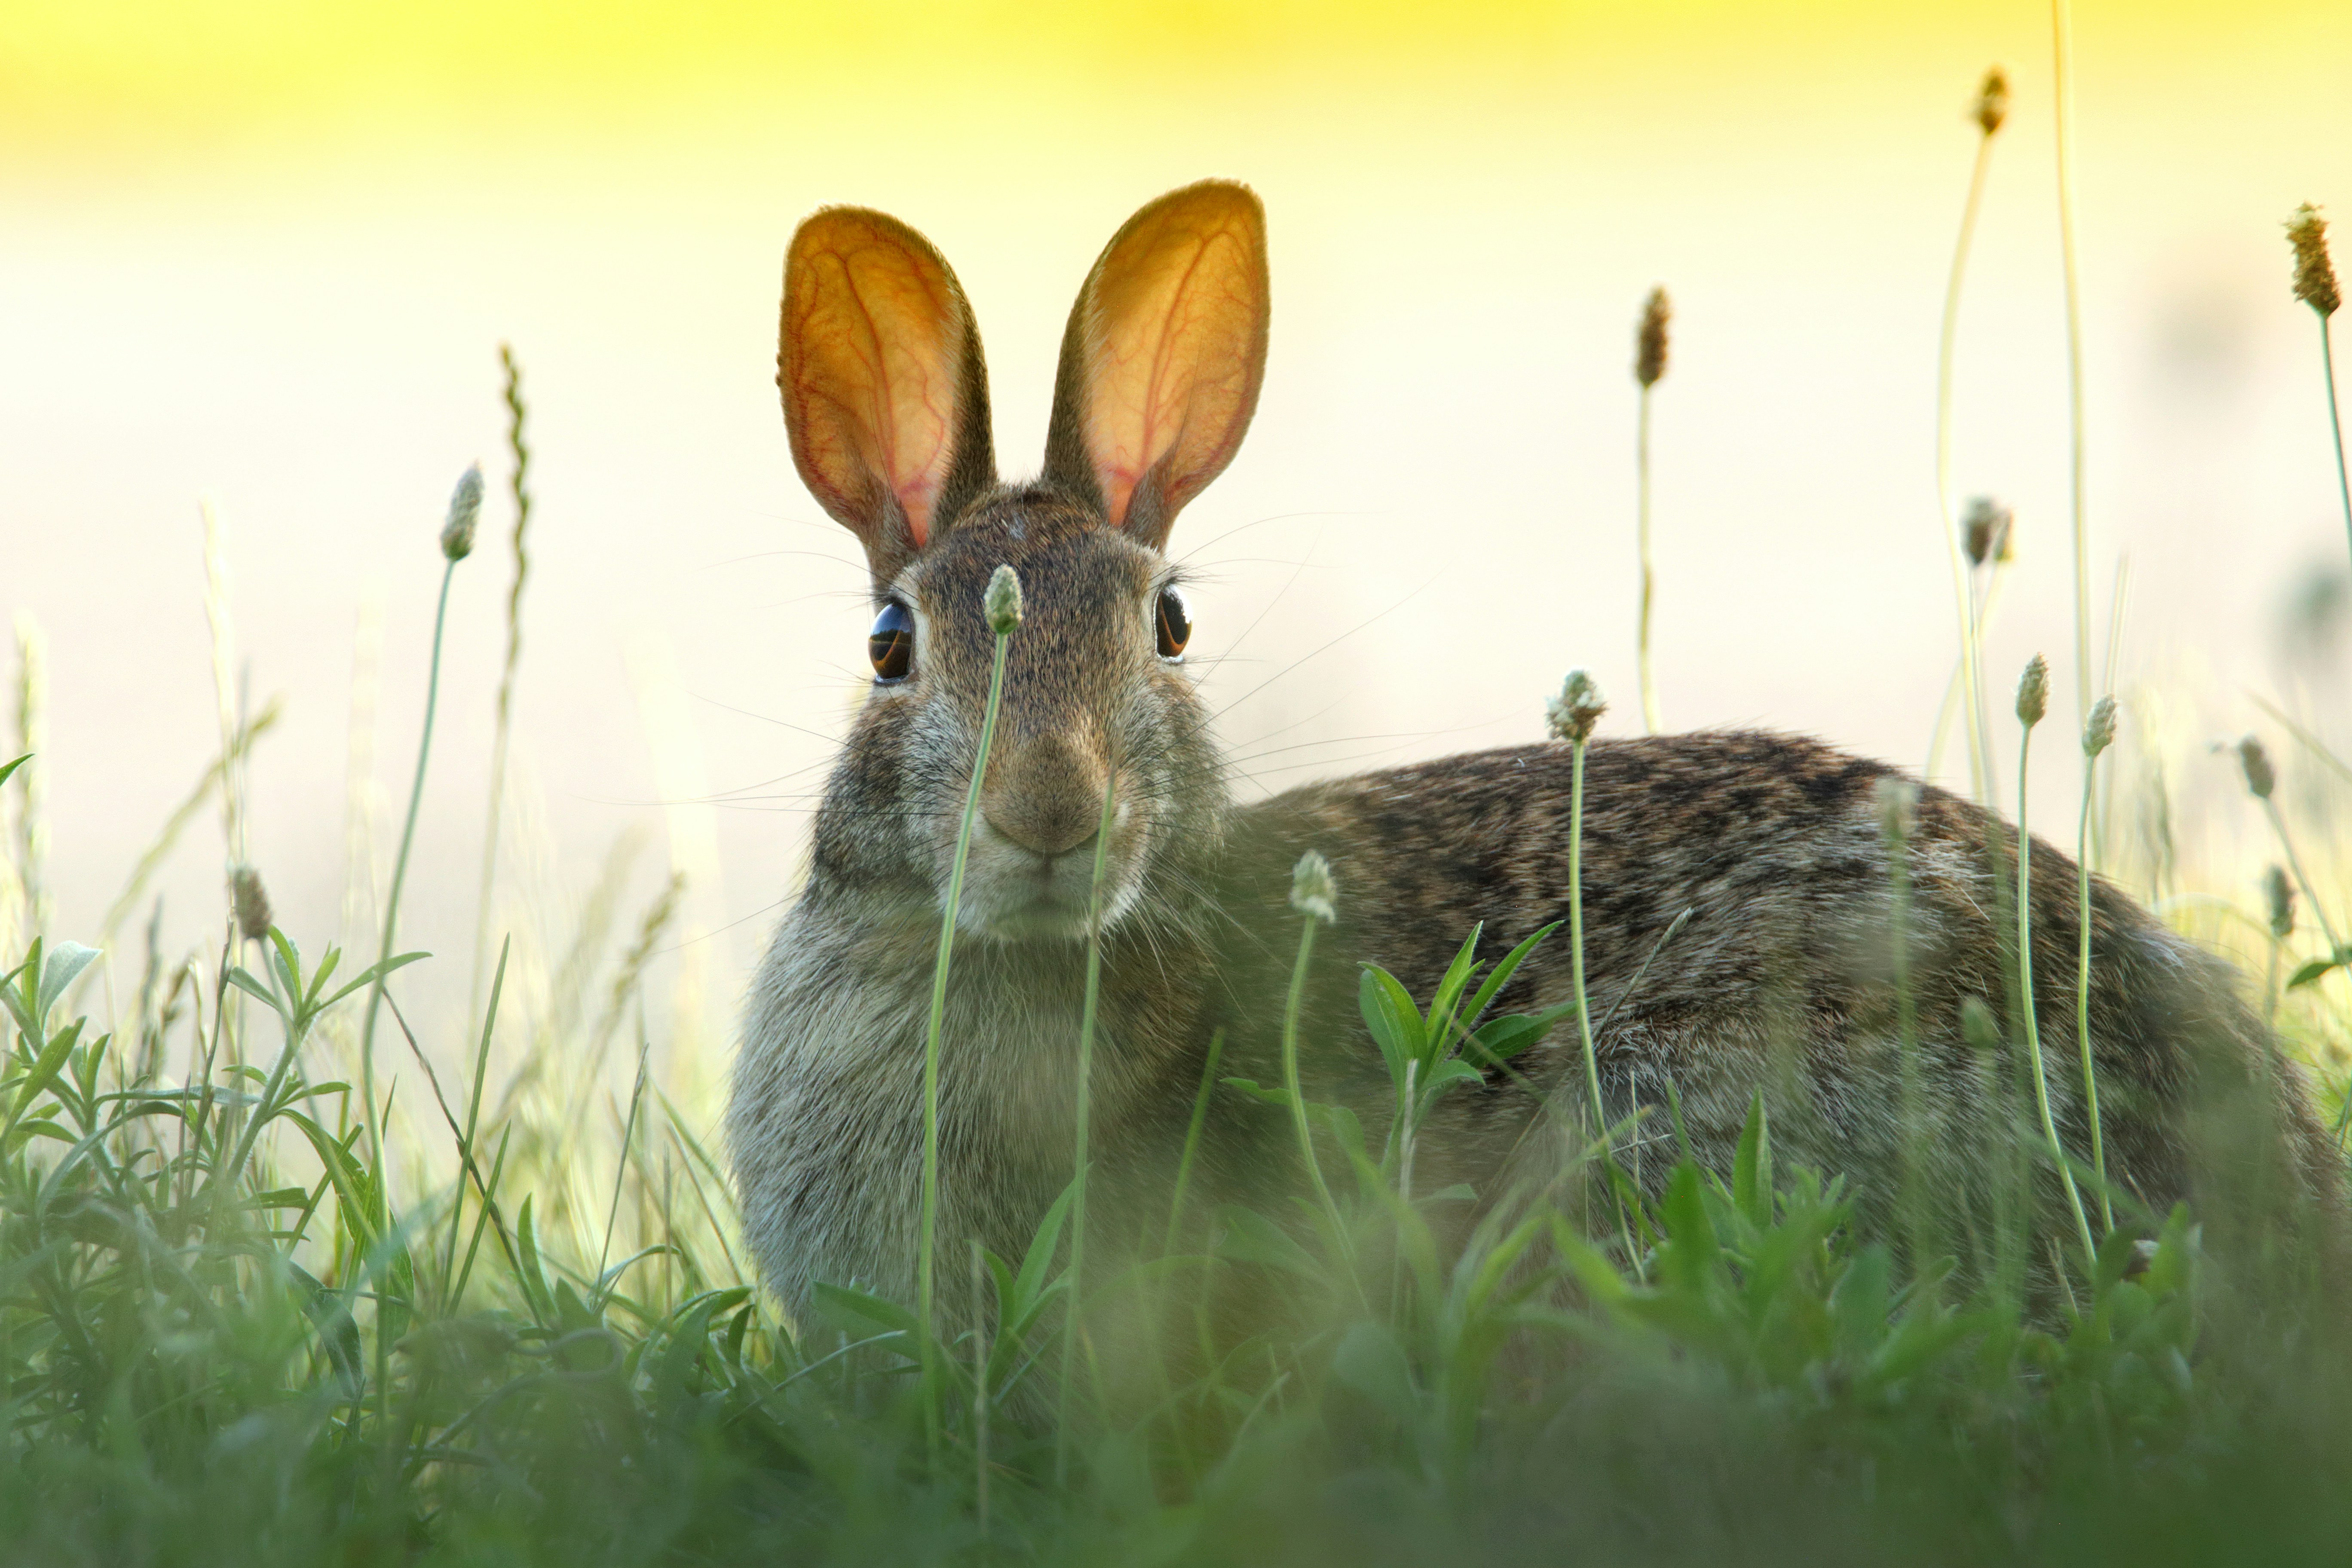
\includegraphics[width=0.9\linewidth,padding=0cm 0cm 0cm 0cm]{graphics/bunny-3.jpg}
        \end{column}
      \end{columns}
    \end{minipage}
  }
  \raisebox{0pt}[0pt][0pt]{
    \begin{minipage}{\textwidth}
      \centering
      \vspace{0.7cm}
      \hspace{1.3cm}\tikz\node[rectangle,fill opacity=1,fill=white,minimum height=4em, text width=0.38\linewidth]{
        \Large
        \hspace{0.1cm}Protocol level DOS
      };
    \end{minipage}
  }

  % \begin{itemize}
  %   \item Attacker trying to perform a protocol-level DOS attack
  %   \item Attacker may observe messages
  %   \item Attacker may insert messages, but they may not drop or modify messages
  %   \item Halfway between an active and passive attacker:
  %   \begin{itemize}
  %   \item For a fully active attacker state disruption is trivial; they can just drop messages
  %   \end{itemize}
  % \end{itemize}
\end{frame}




\begin{frame}{Retransmission Protection in WireGuard}
\hypertarget{retransmission-protection-in-wireguard}{}
\begin{columns}[fullwidth,T]

  \begin{column}{.5\linewidth}
    \vspace{-0.2cm}
    \rlap{\includegraphics[width=1.08\linewidth,page=3,clip=true,trim=0cm 2cm 0cm 1.9cm]{graphics/rosenpass-attack-types.pdf}}
  \end{column}

  \begin{column}{.46\linewidth}
    \vspace{0.4cm} % Manual alignment with blue box in graphic
    \begin{itemize}
      \item Replay attacks thwarted by counter
      \item Counter is based on real-time clock
      \item Responder is semi-stateful (one retransmission at program start may be accepted, but this does not affect protocol security)
      \item[$\Rightarrow$]
         WG requires \emph{either} reliable real-time clock \emph{or} stateful initiator
      \item[$\Rightarrow$]
        Adversary can attempt replay, but this cannot interrupt a valid handshake by the initiator
      \item[!] Assumption of reliable system time is invalid in practice!
    \end{itemize}
  \end{column}
\end{columns}
\end{frame}




\begin{frame}{ChronoTrigger Attack}
\begin{columns}[fullwidth,T]
  \begin{column}{.5\linewidth}
    \vspace{-0.2cm}
    \rlap{\includegraphics[width=1.08\linewidth,page=5,clip=true,trim=0cm 2cm 0cm 1.9cm]{graphics/rosenpass-attack-types.pdf}}
  \end{column}

  \begin{column}{.46\linewidth}
    \small\leavevmode
    \only<+|handout:+>{
      \begin{enumblock}{Preparation phase:}
      \begin{enumerate}
        \item \textbf{Attacker} sets \emph{initiator system time} to a future value
        \item \textbf{Attacker} records \emph{InitHello} as \emph{KillToken} while both peers are performing a valid handshake
      \end{enumerate}
      \end{enumblock}
\centerline{ \small … both peers are being reset … }
      \begin{enumblock}{Delayed execution phase:}
      \begin{enumerate}
        \item \textbf{Attacker} sends \emph{KillToken} to responder, setting their timestamp to a future value
        \item[$\Rightarrow$] Initiation now fails again due to timestamp mismatch
      \end{enumerate}
      \end{enumblock}
    }

    \only<+|handout:+>{%
      \begin{block}{Gaining access to system time:}
      \begin{itemize}
        \item Network Time Protocol is insecure,\\
        Mitigations are of limited use
        \item[$\Rightarrow$] Break NTP \emph{once}; kill token lasts forever
      \end{itemize}
      \unskip
      \end{block}
    }

    \only<+|handout:+>{%
      \leavevmode\begin{block}{Attacker gains}
      \begin{itemize}
        \item Extremely cheap protocol-level DOS
      \end{itemize}
      \unskip
      \end{block}

      \begin{block}{Preparation phase, attacker needs:}
      \begin{itemize}
        \item Eavesdropping of initiator packets
        \item Access to system time
      \end{itemize}
      \unskip
      \end{block}

      \begin{block}{Delayed execution, attacker needs:}
      \begin{itemize}
        \item No access beyond message transmission to responder
      \end{itemize}
      \unskip
      \end{block}
  }
  \end{column}
\end{columns}
\end{frame}




\begin{frame}{ChronoTrigger: Changes in Rosenpass}
  \begin{columns}[fullwidth,c]

    \begin{column}{.2\linewidth}
      \vspace{-0.2cm}
      \rlap{\includegraphics[height=\textheight,page=7,clip=true,trim=0.5cm 0.1cm 13cm 3cm]{graphics/rosenpass-attack-types.pdf}}
    \end{column}

    \begin{column}{.2\linewidth}
      \vspace{-0.2cm}
      \rlap{\includegraphics[height=\textheight,page=7,clip=true,trim=13cm 0.1cm 0.5cm 3cm]{graphics/rosenpass-attack-types.pdf}}
    \end{column}

    \begin{column}{.56\linewidth}
      \begin{itemize}
        \item InitHello is unauthenticated because responder still needs to encapsulate secret with initiator key
        \item Since InitHello is unauthenticated, retransmission protection is impossible
        \item Responder state is moved into a cookie called \emph{Biscuit}; this renders the responder stateless
        \item Retransmission of InitHello is now easily possible, but does not lead to a state disruption attack
        \item[$\Rightarrow$] Stateless responder prevents ChronoTrigger attack
      \end{itemize}
    \end{column}
  \end{columns}
\end{frame}




\begin{frame}{Rosenpass Key Derivation Chain: Spot the Biscuit}
  \hypertarget{rosenpass-kdf-chain-spot-the-biscuit}{}
  \centering
  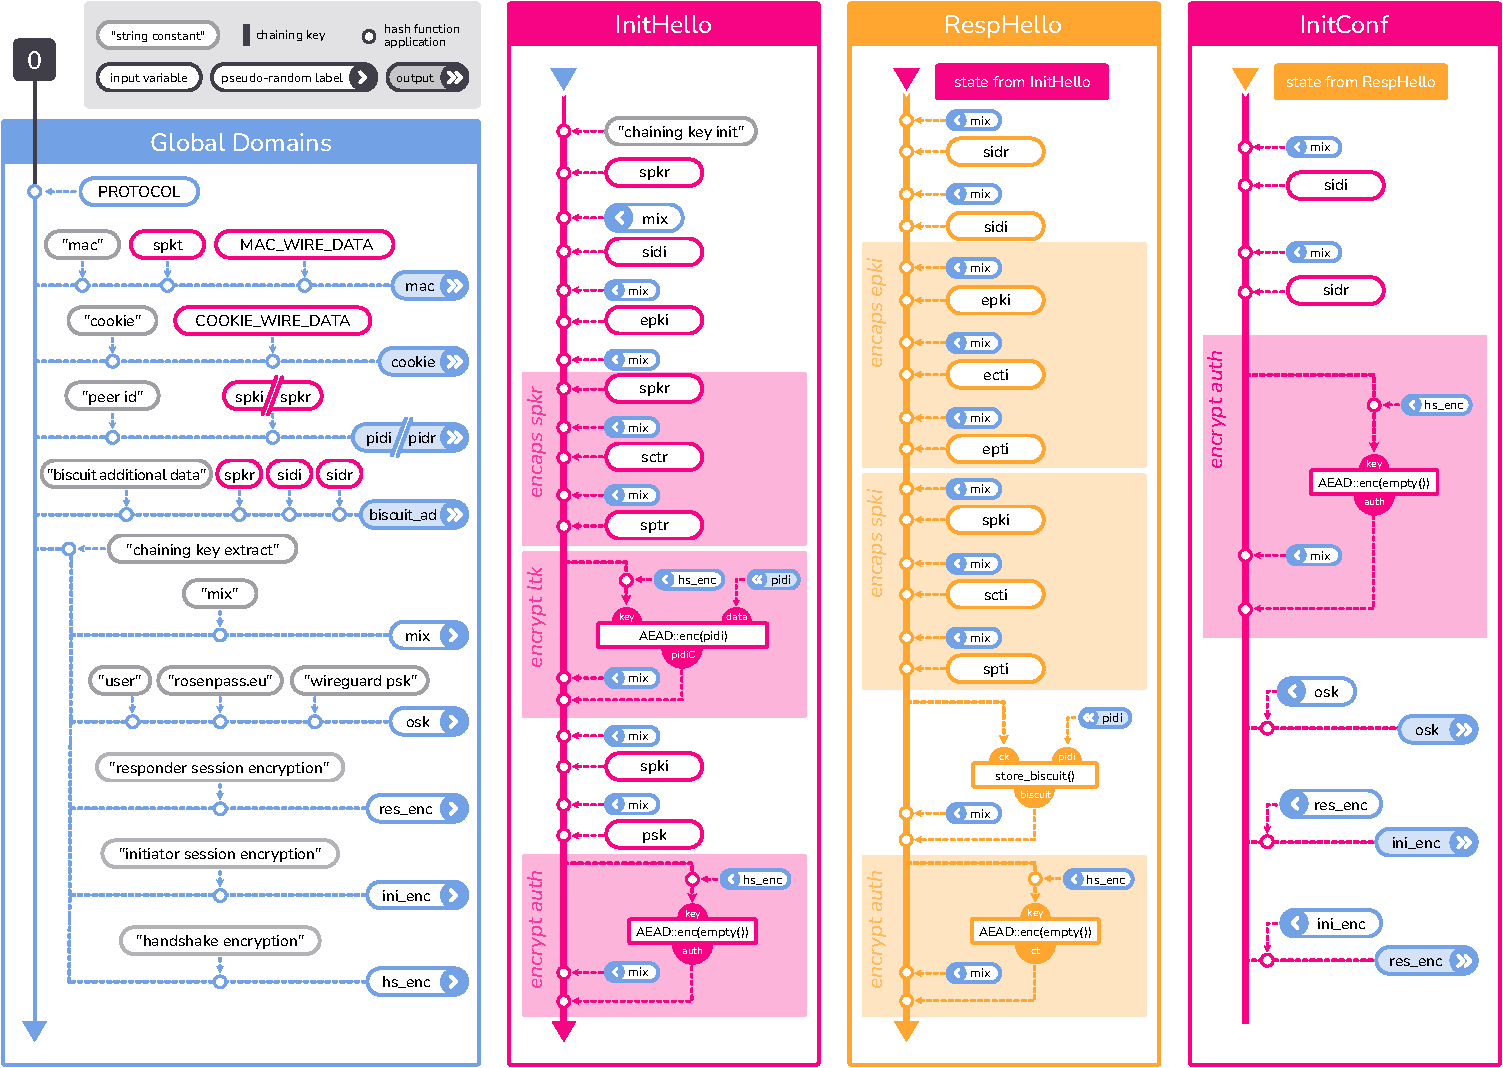
\includegraphics[height=.85\textheight]{graphics/rosenpass-wp-hashing-tree-rgb.pdf}
\end{frame}




\begin{frame}{Rosenpass Protocol Messages: Spot the Biscuit}
  \hypertarget{rosenpass-protocol-messages-spot-the-biscuit}{}
    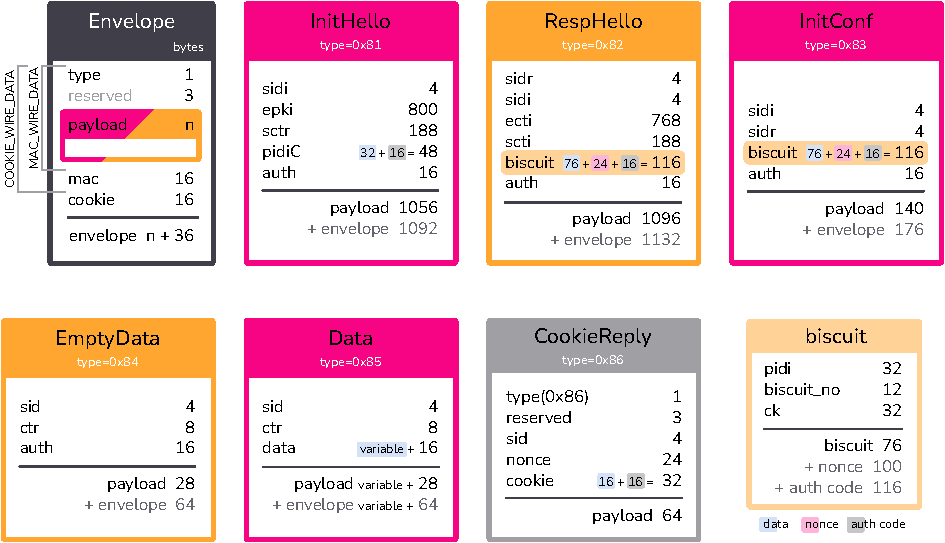
\includegraphics[height=.85\textheight]{graphics/rp-messages-04-all-rgb.pdf}
\end{frame}

\interlude*<left,leftskip=7cm,>[90]<Tribulations \textasciitilde\ Tooling>{Oh These\\Proof Tools}<Vive la Révolution! Against the Bourgeoisie of Proof Assistants!>
\section{Section: Better proof tools}

\begin{frame}[T]{Pen and Paper}
  \begin{columns}[fullwidth,t]
    \begin{column}{.29\linewidth}
      \raisebox{\dimeval{-\height}}{
\includegraphics[width=\linewidth]{graphics/this-is-fine-crop.png}}\par\nointerlineskip
      
\includegraphics[width=\linewidth]{graphics/this-is-not-fine-crop.jpg}%
    \end{column}
    \hfill
    \begin{column}{.68\linewidth}
      \small

\begin{description}[]
\item[{Bellare and Rogaway: [BR06]}]\leavevmode\newline many \enquote{essentially unverifiable} proofs, \enquote{crisis of rigor}

\item[{Halevi: [Hal05]}]\leavevmode\newline
	some reasons are social,
but \enquote{our proofs are truly complex}

%\item[{Joseph Jaeger: [ProTeCS 2024, Workshop at Eurocrypt]}]\leavevmode\newline
%technical and social reasons
%why and for whom do we write proofs?

%\item[We'd like to add:]\leavevmode\newline
%pen-and-paper proofs are hard to maintain, update, reuse
%especially for 3rd parties

%Can proofs become part of a continuous engineering effort?
\end{description}
    \end{column}
  \end{columns}
\end{frame}

\setbeamercolor{overlaybox}{bg=white}
\begin{frame}{Symbolic Modeling of Rosenpass}
  \begin{columns}[c]
    \begin{column}{.5\linewidth}
     \hspace*{-\UseName{beamer@leftmargin}}\rlap{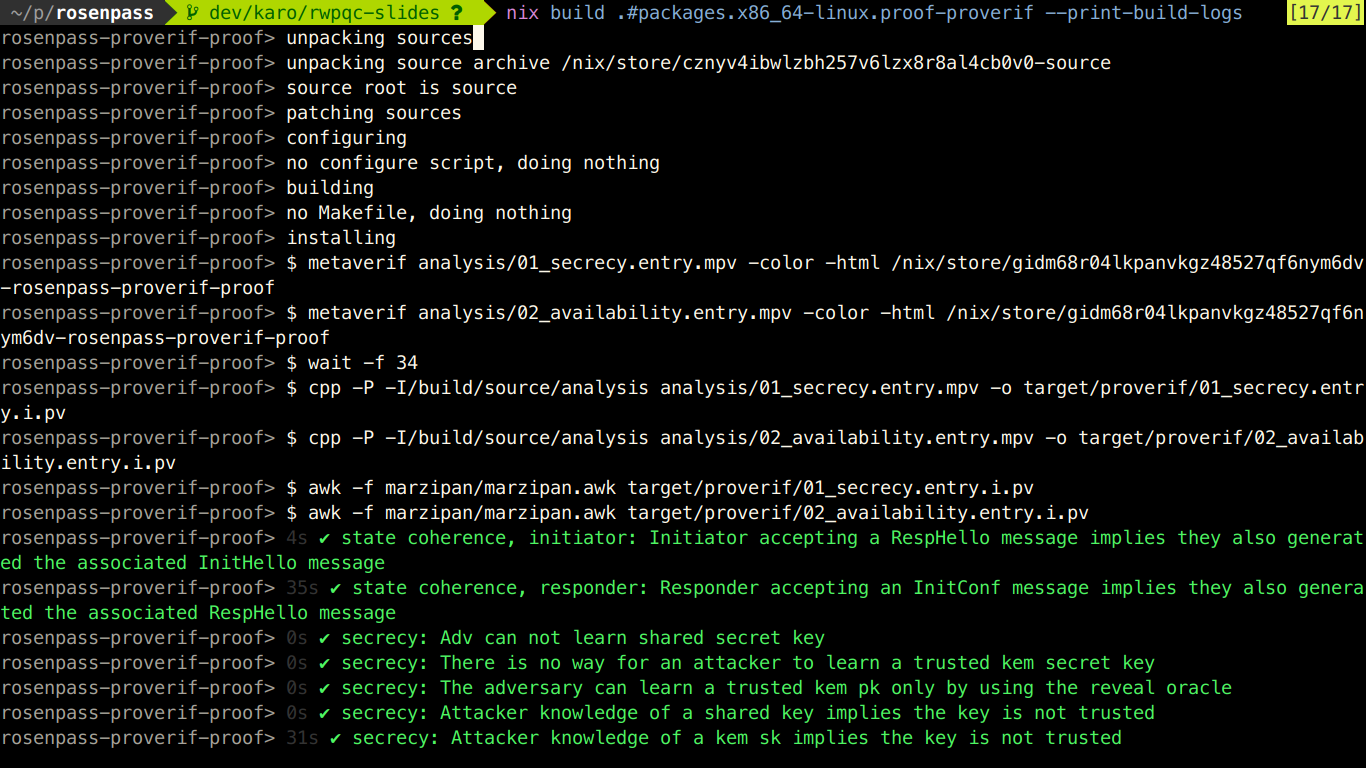
\includegraphics[keepaspectratio,height=\defaultframetextheight]{graphics/2023-03-20-symbolic-analysis-screenshot.png}}
    \end{column}%
	  %\pause
    \begin{column}{.5\linewidth}
    \begin{beamercolorbox}[colsep*=1ex,ht=\dimeval{\defaultframetextheight+2pt}]{overlaybox}
      \begin{itemize}
        \item symbolic modeling using ProVerif
        \item proofs treated as part of the codebase
        \item uses a model internally that is based on a fairly comprehensive Maximum Exposure Attacks (MEX) variant
        \item covers non-interruptability (resistance to disruption attacks)
        \item mechanized proof in the computational model is an open issue
      \end{itemize}
  \end{beamercolorbox}
    \end{column}
  \end{columns}
\end{frame}




% \begin{frame}{Friction \& Frustration for the Working Cryptographer}
%   \textbf{Tooling}
%   \begin{itemize}
%     \item Syntax highlighting, favorite editor
%     \item Engineering for large models: syntax rewriting, syntactic sugar, macros
%     \item Comfortable tooling to inspect intermediate games (CryptoVerif)
%   \end{itemize}
%   \vspace{1em}
%   \textbf{Documentation:} Often incomplete; step from example to research too big\\[.8em]

%   \textbf{Output:} hard to understand for non-experts\\[.8em]

%   \textbf{Input Language:} Unintuitive? Inaccessible? Mixed signals!\\[.8em]

%   \textbf{Proof Language:} not enough flexibility and leeway compared to pen-and-paper
%   \begin{itemize}
%     \item hand-waving, unsafe blocks
%       % pen-and-paper get way more leeway, mechanized proofs are often all or nothing
%     \item support for incremental process
%   \end{itemize}
% \end{frame}



% \begin{frame}{The Day Language Came into My Life}

%   %$\dots$ and mechanised proofs have not covered this thus far.

%   %\vspace{5em}

%   \blockquote[Helen Keller (1880--1968) in The Day Language Came into My Life]{
%     Everything had a name, and each name gave birth to a new thought.
%   }

% % We do not want to be typecast into people who just do usability or accessibility

% % language creates awareness, consciousness

% % neces. prerequisite

% % in order to be able to reason mathematically

% % math is the process of giving, of express math
% % concepts in the form of language
% %

% % math is something fundamentally kommunikatives

% % that's an aspect that mechanised proofs haven't covered thus far

% % Everything had a name, and each name gave birth to a new thought.
% % --- Helen Keller (1880--1968) in The Day Language Came into My Life


% % https://www.pval.org/cms/lib/NY19000481/Centricity/Domain/105/The%20Day%20Language%20Came%20into%20my%20Life.pdf

% \end{frame}










\begin{frame}{Rosenpass going Rube-Goldberg}
  \begin{columns}[fullwidth]
    \begin{column}{.7\linewidth}
      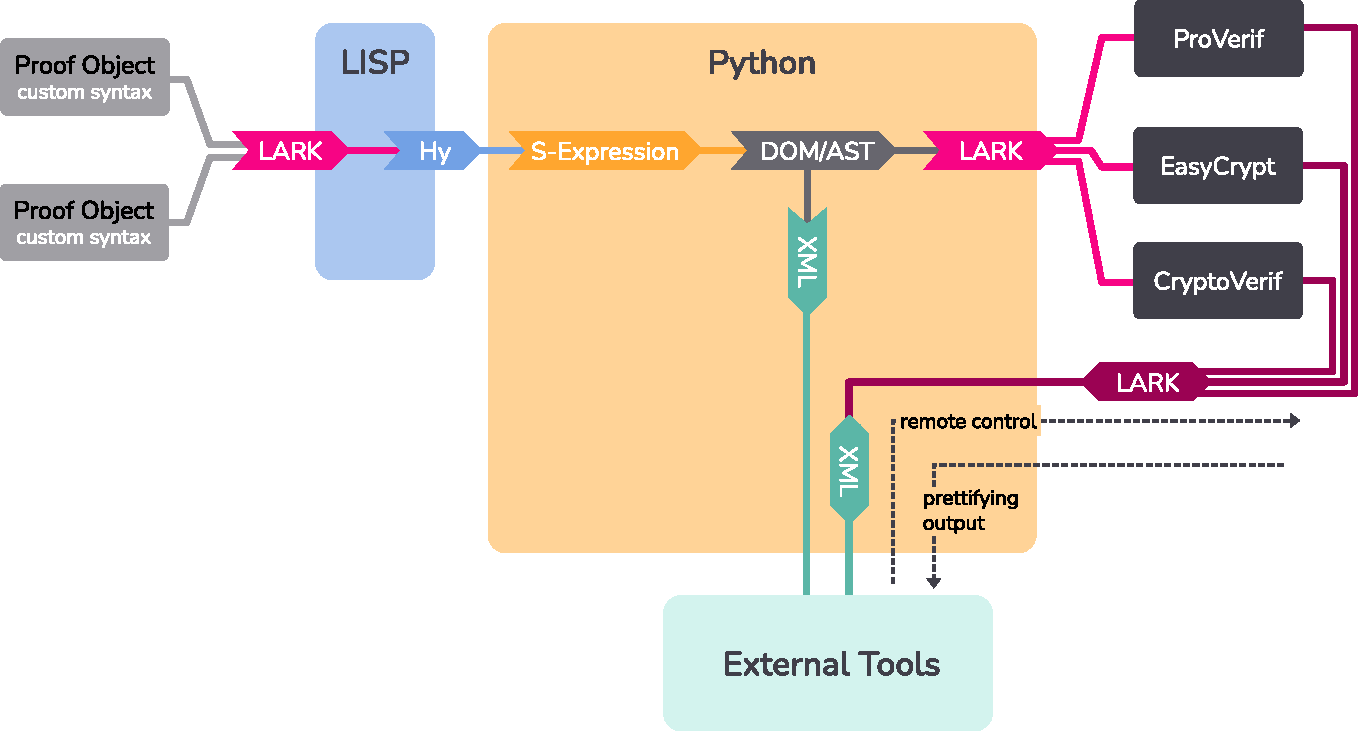
\includegraphics[width=\linewidth]{graphics/python-proofs.pdf}
    \end{column}\hfill
    \begin{column}{.28\linewidth}
\stretchcolumn{
      \textbf{We will} build a framework around existing tools
      \vfil

      \textbf{Keep} expressivity and preciseness

      \vfil
      \textbf{Generate and Parse} their languages

      \vfil
      \textbf{Open them up} to ecosystems in Python, Lisp, XML

	\vfil
}
    \end{column}

  \end{columns}
\end{frame}

\interlude[7]{Epilogue}

\begin{frame}[T]{Epilogue}
  \begin{columns}[fullwidth]
    \begin{column}{.3\linewidth}
	\stretchcolumn{
      \begin{block}{Rosenpass\strut}
      \small
        \begin{itemize}
          \item Post-quantum secure AKE
          \item Same security as WireGuard
          \item Improved state disruption resistance
          \item Transfers key to WireGuard for hybrid security
        \end{itemize}
      \end{block}
	\vfill
        \hfill\textbf{\url{rosenpass.eu}}
	}
    \end{column}

    \begin{column}{.3\linewidth}
	\stretchcolumn{
      \begin{block}{About Protocols\strut}
      \small
        \begin{itemize}
          \item It is possible to treat NIKEs as KEMs with DHKEM
          \item The GHP Combiner can be used to combine multiple KEMs
          \item X-Wing makes this easy
          \item Wall clocks are not to be trusted
        \end{itemize}
      \end{block}
\vfill
}
    \end{column}

    \begin{column}{.3\linewidth}
\stretchcolumn{
      \begin{block}{Talk To Us\strut}
      \small
        \begin{itemize}
          \item Adding syntax rewriting to the tool belt of mechanized verification in cryptography
          \item Using broker architectures to write more secure system applications
          \item Using microvms to write more secure applications
          \item More use-cases for rosenpass
        \end{itemize}
      \end{block}
\vfill
}
    \end{column}
  \end{columns}
\end{frame}

% reset backgorund canvas
\setbeamertemplate{background canvas}{}
\interlude[7]{
  Appendix --- Here Be Dragons
}

\begin{frame}{Bibliography}
  \begin{description}
    \item[\citePqwg:] \url{\citePqwgUrl}
  \end{description}
\end{frame}

\begin{frame}{Graphics attribution}
  \tiny
  \begin{itemize}
    \item \url{https://unsplash.com/photos/brown-rabbit-Efj0HGPdPKs}
    \item \url{https://unsplash.com/photos/barista-in-apron-with-hands-in-the-pockets-standing-near-the-roaster-machine-Y5qjv6Dj4w4}
    \item \url{https://unsplash.com/photos/a-small-rabbit-is-sitting-in-the-grass-1_YMm4pVeSg}
    \item \url{https://unsplash.com/photos/yellow-blue-and-black-coated-wires-iOLHAIaxpDA}
    \item \url{https://unsplash.com/photos/gray-rabbit-XG06d9Hd2YA}
    \item \url{https://unsplash.com/photos/big-ben-london-MdJq0zFUwrw}
    \item \url{https://unsplash.com/photos/white-rabbit-on-green-grass-u_kMWN-BWyU}
  \end{itemize}
\end{frame}


%\interlude[7]{
  Random slides --- The dragon just ate you!
}

% \begin{frame}{Hybrid Security with WireGuard}
% \begin{itemize}
% \item
%   Hybrid post-quantum security due to integration with WireGuard
% \item
%   Session keys produced by Rosenpass used in WireGuard as PSKs
% \item
%   Continuous key renegotiation, every 2 minutes, like WireGuard

%   \begin{itemize}
%   \item
%     When Rosenpass fails to exchange a key, we randomize the WireGuard
%     PSK to make WireGuard fail, too
%   \end{itemize}
% \item
%   This negates some of our advancements in regards to state disruption
%   resistance compared to standalone WireGuard
%
%   \begin{itemize}
%   \item
%     We feel it is worth it though
%   \end{itemize}
% \end{itemize}
% \end{frame}

% \begin{frame}{Rosenpass Usability Goals}
% \hypertarget{rosenpass-usability-goals}{}
% % :information\_source: (done) Insert infographic kem value naming scheme
% % (sski/spki/\ldots)
% % :information\_source: (done) Insert Infographic ID naming
% % scheme (pidi, sidr)

% % TODO(blipp,marei) fix the layout to something that works
% %                   Questions to Marei: what kind of object is
% %                   a tikzpicture? Why can't I do a newline after one?
%   \begin{columns}[c]
%     \begin{column}{.5\textwidth}

%       \resizebox{.9\textwidth}{!}{%
%         \begin{namepartpicture}
%         \namepart{s=Static,e=Ephemeral}
%         \namepart[3.5cm]{sk=Secret Key,pk=Public Key,pt=Plaintext,ct=Ciphertext}
%         \namepart[7cm]{i=Initiator,r=Responder,m=Mine,t=Theirs}
%         \begin{scope}[decoration={brace,amplitude=5mm},thick]
%         \namebraceright{s}{e}
%         \namebraceleft{sk}{ct}
%         \namebraceright{sk}{ct}
%         \namebraceleft{i}{t}
%         \end{scope}
%         \end{namepartpicture}
%       }

%       \resizebox{.9\textwidth}{!}{%
%         \begin{namepartpicture}
%         \namepart{sid=Session ID, pid=Peer ID}
%         \namepart[3.5cm]{i=Initiator,r=Responder,m=Mine,t=Theirs}
%         \begin{scope}[decoration={brace,amplitude=5mm},thick]
%         \namebraceright{sid}{pid}
%         \namebraceleft{i}{t}
%         \end{scope}
%         \end{namepartpicture}
%       }
%     \end{column}

%     \begin{column}{.5\textwidth}

%       \begin{itemize}
%       \item
%         Focus on being particularly reader-friendly
%       \item
%         Our communication targets non-cryptographers, too
%       \item
%         Somewhat speaking variable names
%       \end{itemize}

%     \end{column}
%   \end{columns}
% \end{frame}

\begin{frame}{Rosenpass and WireGuard: Advanced Security}
\hypertarget{wireguard-advanced-security-properties}{}
\vspace{-\ht\strutbox}
\begin{columns}[fullwidth,T]
  \begin{column}{.49\linewidth}
  \begin{block}{Limited Stealth:\strut}
    \begin{itemize}
      \item Protocol should not respond without pre-auth.
      \item Proof of IP ownership (cookie mechanism) prevents full stealth
      \item Adv. needs to know responder public key
    \end{itemize}
    \end{block}

    \begin{block}{Limited Identity Hiding:\strut}
    \begin{itemize}
      \item Adversary cannot recognize peers unless their public key is known
      \item This is incomplete!
    \end{itemize}
    \end{block}
    % TODO(blipp,karo) why can the adversary not produce a proof?
    %   -- Because the recipient public key could be known by anyone -- karo
  \end{column}

  \begin{column}{.49\linewidth}
    \begin{block}{CPU DOS mitigation:\strut}
    % TODO(blipp,karo) why is it limited? 
    %  -- Because an attacker who knows the public keys can still cause 
    \begin{itemize}
      \item Attacker should not easily trigger public key operations
      \item Preventing CPU exhaustion using network amplification
      \item Proof of IP ownership
    \end{itemize}
    \end{block}

    % \textbf{Interruption resistance:} \vspace{0.5em} % TODO(blipp): Mark red somehow?
    % \begin{itemize}
    %   \item Replay protection based on counters
    %   \item Attacks exist in WireGuard
    %   \item Explicit modeling \& security is a goal in Rosenpass
    % \end{itemize}
    % TODO(blipp,karo) decide how to format the tradeoffs line
    %\item
    %  =\textgreater{} These properties are tradeoffs
  \end{column}
\end{columns}
\end{frame}

% \begin{frame}{Rosenpass Security Properties}
% \hypertarget{rosenpass-security-properties}{}

% % TODO(blipp) Make this look more balanced
% % TODO(marei) can the items start further on the left, i.e., no padding on the left?
% % TODO(marei) if this does not solve the space problem, what else could we do to make "Post-Quantum Security" fit into one line in the first column, and the footnote marks in columns 2 and 3?
% % TODO(marei) colors green and red for checkmark and cross?
% % :information\_source: (done) Formosa Retreat slides, slide 2
% \vspace{0.5em}
% \begin{columns}[t]
% \begin{column}{.33\textwidth}
% \heading{WireGuard}
% \begin{itemize}
%   \itemtick Session-key secrecy
%   \itemtick \dots
%   \itemtick Identity Hiding
%   \itemfail \textbf{Non-Interruptability} \footnote[frame]{Assuming a trusted system time}
%   \itemfail \textbf{Post-Quantum Security}
% \end{itemize}
% \end{column}

% \begin{column}{.33\textwidth}
% \heading{
%   PQ WireGuard
%   \footnote[frame]{
% 	  Hülsing, Ning, Schwabe, Weber, Zimmermann. “Post-quantum WireGuard”. https://ia.cr/2020/379
% 	}
% }
% \begin{itemize}
%   \itemtick \textbf{Post-Quantum Security}
%   \itemfail \textbf{Hybrid security}
%   \itemfail \textbf{Non-Interruptability} \footnote[frame]{Assuming a PSK}
% \end{itemize}
% \end{column}

% \begin{column}{.33\textwidth}
% \heading{Rosenpass}
% \begin{itemize}
%   \itemtick \textbf{Non-Interruptability} \footnote[frame]{Through cookies}
%   \itemtick \textbf{Hybrid security} \footnote[frame]{Used together with standard WireGuard}
% \end{itemize}
% \end{column}

% \end{columns}
% \vspace{1.5em}

% \end{frame}

%TODO(marei) Can this code be better/more LaTeX-y?
\interlude[1]<Triumphs \textasciitilde\ Secrecy \& Non-Interruptability>{Modeling of Rosenpass}<Using ProVerif>

% TODO Blipp: Insert example as discussed
% \begin{frame}{Symbolic modeling: Exposure scenario enumeration}
% \hypertarget{analysis-usability-colorful-proverif-voice}{}
% \begin{itemize}
%   \item Covers a broad range of exposure scenarious
%   \item Plain listing of minimum conditions for secrecy of the output key to hold
%   \item Modeling of various exposure scenarious such as ephemeral key and both peer keys being the same key
% \end{itemize}
% \end{frame}

\begin{frame}{Non-Interruptability: More Formally}
    For every pair of traces $\mathtt{tmin}, \mathtt{tmax}$ where trace $\mathtt{tmax}$ can be formed by
    insertion of messages/oracle calls into $\mathtt{tmin}$, the result of $\mathtt{tmin}$ and $\mathtt{tmax}$
    should remain the same.

	

    \begin{itemize}
      \item Let $\mathtt{Result}$ be the set of possible protocol results
      \item Let $\mathtt{Trace}$ be the set of possible protocol traces
      \item Let $\mathtt{res}(\mathtt{t}) : \mathtt{Trace} \to \mathtt{Result}$ determine the protocol result given $\mathtt{t} : \mathtt{Trace}$
      \item Let $\mathtt{t1} \supseteq \mathtt{t2} : \mathtt{Trace} \to \mathtt{Trace} \to \mathtt{Prop}$ denote that $\mathtt{t}2$ can be formed by insertion of elements into $\mathtt{t}1$
      \item $\forall (\mathtt{tmin}, \mathtt{tmax}) : \mathtt{Trace} \times \mathtt{Trace}; \mathtt{tmin} \supseteq \mathtt{tmax} \to \mathtt{res}(\mathtt{tmin}) = \mathtt{res}(\mathtt{tmax})$
    \end{itemize}
    \pdfpcnote{Karo}
\end{frame}

% TODO: Blipp. Insert example to explain
% @lemma "non-interruptability: Adv cannot prevent a genuine InitConf message from being accepted"
% lemma ih:InitHello_t, rh:RespHello_t, ic:InitConf_t, psk:key, sski:kem_sk, sskr:kem_sk;
  % event(ICRjct(ic, psk, sskr, kem_pub(sski)))
  % && event(IHSent(ih, psk, sski, kem_pub(sskr)))
  % && event(RHSent(ih, rh, psk, sskr, kem_pub(sski)))
  % && event(ICSent(rh, ic, psk, sski, kem_pub(sskr))).
% \begin{frame}{Symbolic modeling: Non-Interruptability}
% \hypertarget{analysis-usability-colorful-proverif-voice}{}
% \begin{itemize}
%   \item Non-Interruptability is security from disruption attacks
%   \item 
%   % TODO Blipp: Add more formal definition?
% \end{itemize}
% \end{frame}


% \begin{frame}{Rosenpass Security Analysis}
% \hypertarget{rosenpass-security-analysis}{}
% % TODO(marei) see line below
% % :information\_source: Insert proverif in technicolor screenshot in
% % the right side. Cut off. Clearly marked as decoration

% \begin{columns}[c]
%     \begin{column}{.5\textwidth}
%       \begin{itemize}
%       \item
%         Symbolic analysis of Secrecy, Authenticity, and MEX attacks in
%         ProVerif

%         \begin{itemize}
%         \item
%           Novel model of different exposure scenarios
%         \item
%           Essentially listing minimum requirements for security properties to
%           hold
%         \end{itemize}
%       \item
%         Symbolic analysis of State Disruption Resistance in ProVerif

%         \begin{itemize}
%         \item
%           Modeled using ``package accept'' and ``package rejected'' events in
%           the protocol transcript
%         \item
%           Adversary's inability to produce a ``package rejected'' event for a
%           valid handshake message
%         \end{itemize}
%       \end{itemize}

%     \end{column}

%     \begin{column}{.5\textwidth}
%       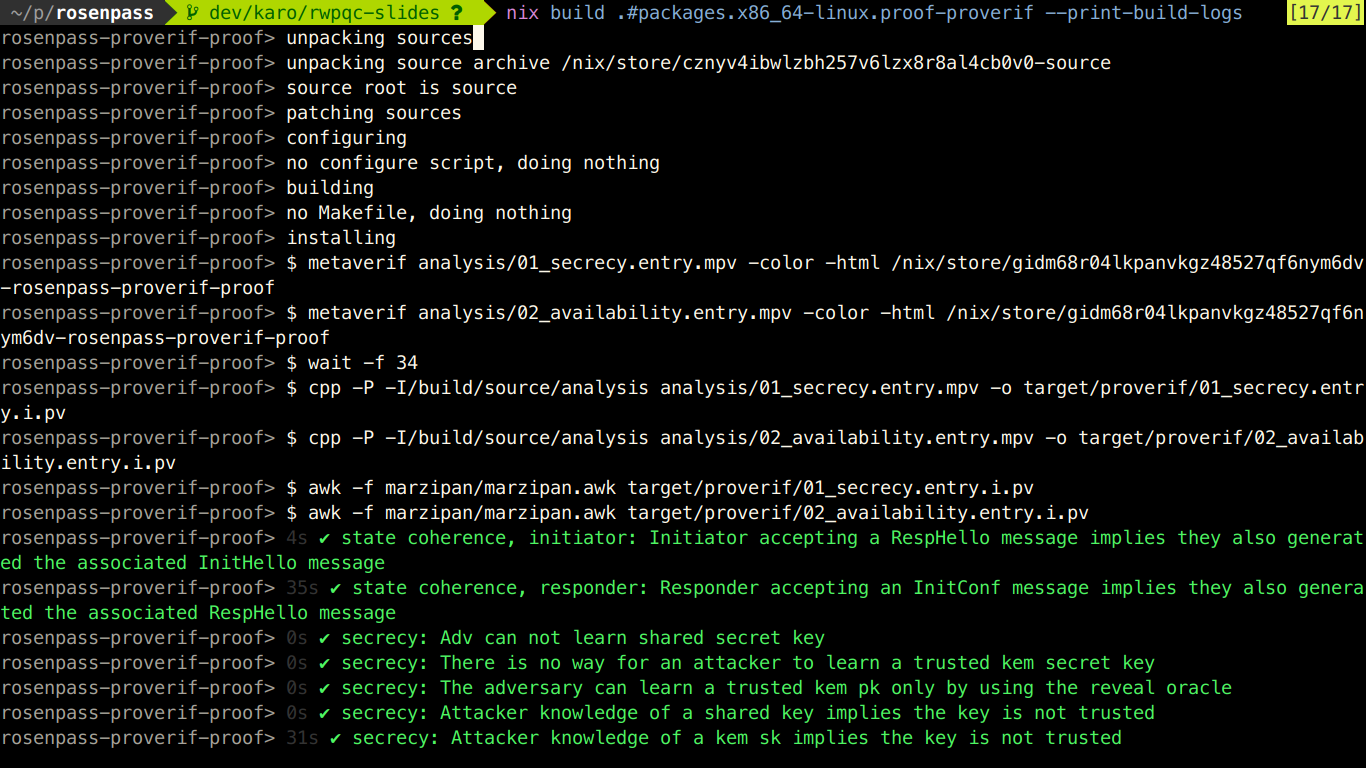
\includegraphics[keepaspectratio,width=.9\textwidth]{graphics/2023-03-20-symbolic-analysis-screenshot.png}

%     \end{column}
%   \end{columns}
% \end{frame}

\begin{frame}{ChronoTrigger Attack: Immediate Execution}
\begin{columns}[fullwidth,T]
  \begin{column}{.5\linewidth}
    \rlap{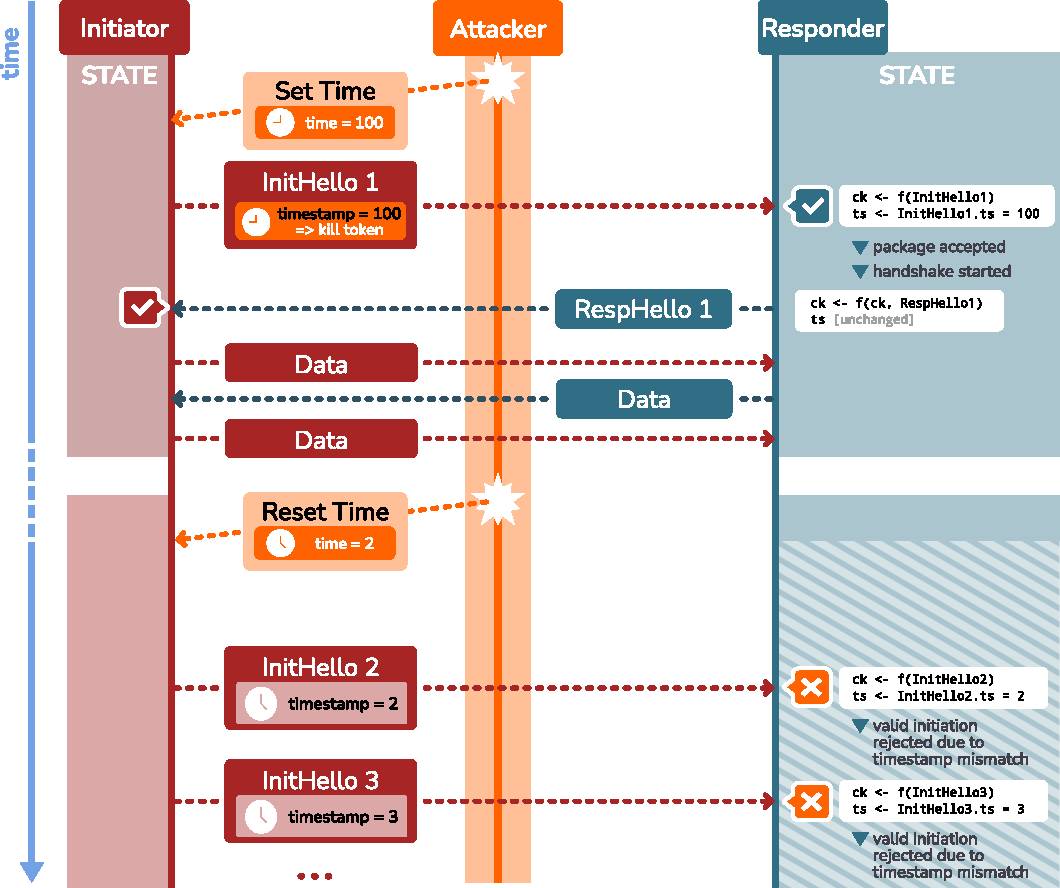
\includegraphics[height=.85\textheight]{graphics/chronotrigger-immediate-bare.pdf}}
  \end{column}

  \begin{column}{.46\linewidth}
    \small\leavevmode
      \begin{enumblock}{Preparation phase:}
      \begin{enumerate}
        \item \textbf{Attacker} sets \emph{initiator system time} to a future value
        \item \textbf{Attacker} waits while both peers are performing a valid handshake
      \end{enumerate}
      \end{enumblock}
      \begin{enumblock}{Direct execution phase:}
      \begin{enumerate}
        \item \textbf{Attacker} lets system time on initiator reset
        \item[=>] Initiation now fails due to counter mismatch
      \end{enumerate}
      \end{enumblock}
  \end{column}
\end{columns}
\end{frame}

\begin{frame}{ChronoTrigger: Changes in Post-Quantum WG}
\hypertarget{wireguard-and-post-quantum-wireguard}{}
  \begin{columns}[fullwidth,T]
    \begin{column}{.5\linewidth}
      \rlap{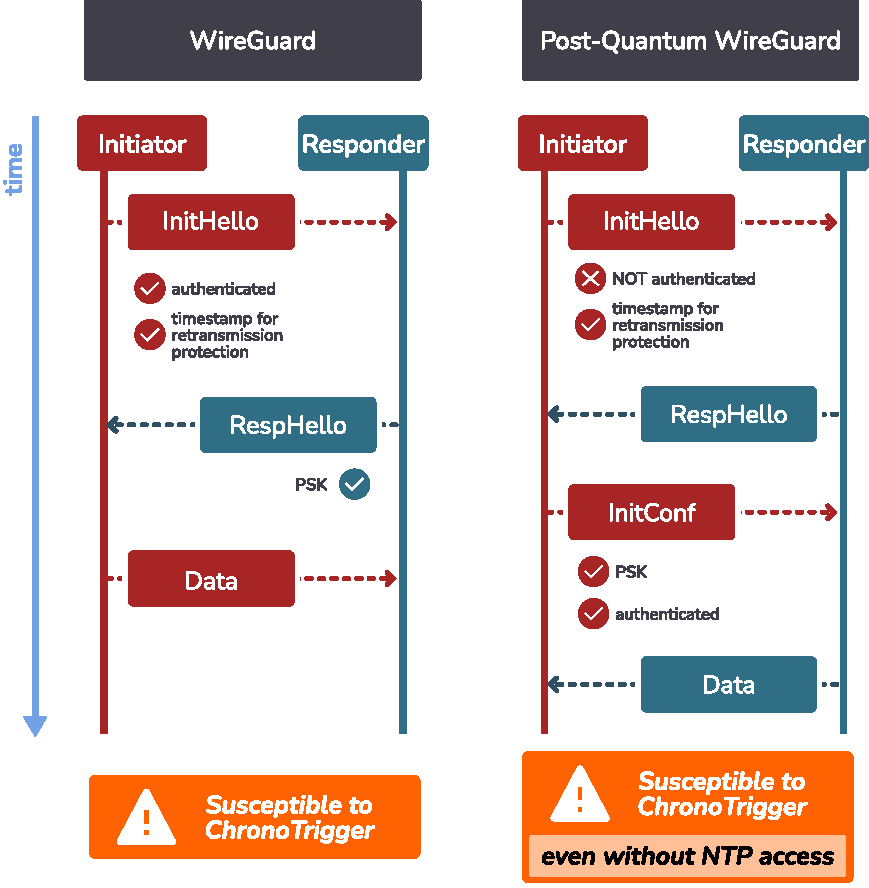
\includegraphics[height=.85\textheight]{graphics/chronotrigger-compare-wg-pqwg.pdf}}
    \end{column}

    \begin{column}{.46\linewidth}
      \begin{itemize}
        \item \emph{InitHello} is unauthenticated
        \item Retransmission counter is kept
        \item PQWG assumes a pre-shared key to authenticate InitHello instead (the authors recommend deriving the PSK from both public keys)
        \item PSK evaluated twice, during InitHello \emph{and} InitConf processing
      \end{itemize}
    \end{column}
  \end{columns}
\end{frame}

\begin{frame}{ChronoTigger against Post-Quantum WireGuard}
  \begin{columns}[fullwidth,T]
    \begin{column}{.5\linewidth}
     \rlap{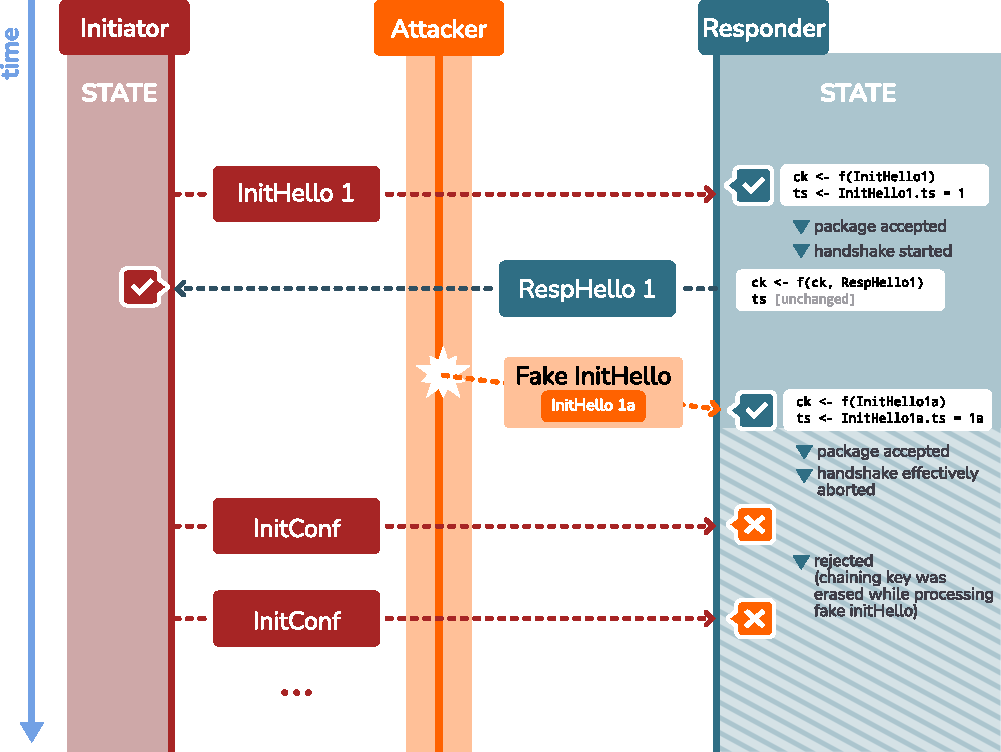
\includegraphics[height=.85\textheight]{graphics/pqwg-state-disrupt-bare.pdf}}
    \end{column}

    \begin{column}{.4\linewidth}
      \begin{block}{No PSK/Public keys as PSK}
      \begin{itemize}
        \item Attacker needs access to public keys
        \item The attack is trivial (attacker just forges \emph{InitHello})
      \end{itemize}
      \end{block}

      \begin{block}{With PSK}
      \begin{itemize}
        \item Replay attack with NTP access from classic WireGuard still applies
      \end{itemize}
      \end{block}
    \end{column}
  \end{columns}
\end{frame}

\interlude[3]<Trials \textasciitilde\ Attacks found>{CookieCutter}

\begin{frame}{CookieCutter Attack}
\hypertarget{cookiecutter-attack}{}
\only<+|handout:+>{
    \begin{columns}[fullwidth,c]
      \begin{column}{.5\linewidth}
        \blockquote[\textbf{A WireGuard CookieReply}, ca. 2014]{
          I am under load. Prove that you are not using IP address impersonation before I process your handshake! 

          This message contains a \emph{cookie key}. Use it to prove that you can receive messages sent to your
          address when retransmitting your \emph{InitHello} packet.}
      \end{column}

      \begin{column}{.4\linewidth}
        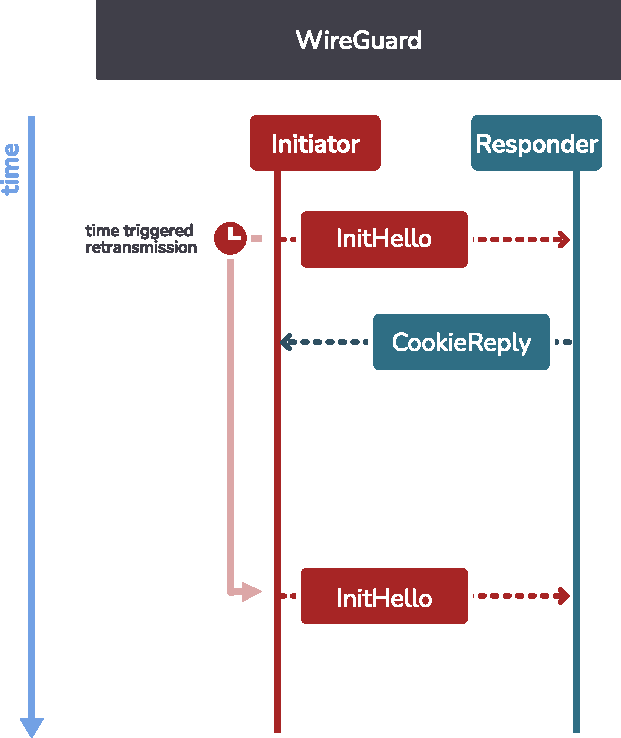
\includegraphics[height=.85\textheight]{graphics/wg-cookiereply.pdf}
      \end{column}
    \end{columns}
  }


    \begin{columns}[fullwidth,T]
      \begin{column}<+-|handout:+->{.4\linewidth}
        % TODO(marei) could we avoid that the picture jumps in its vertical position?
        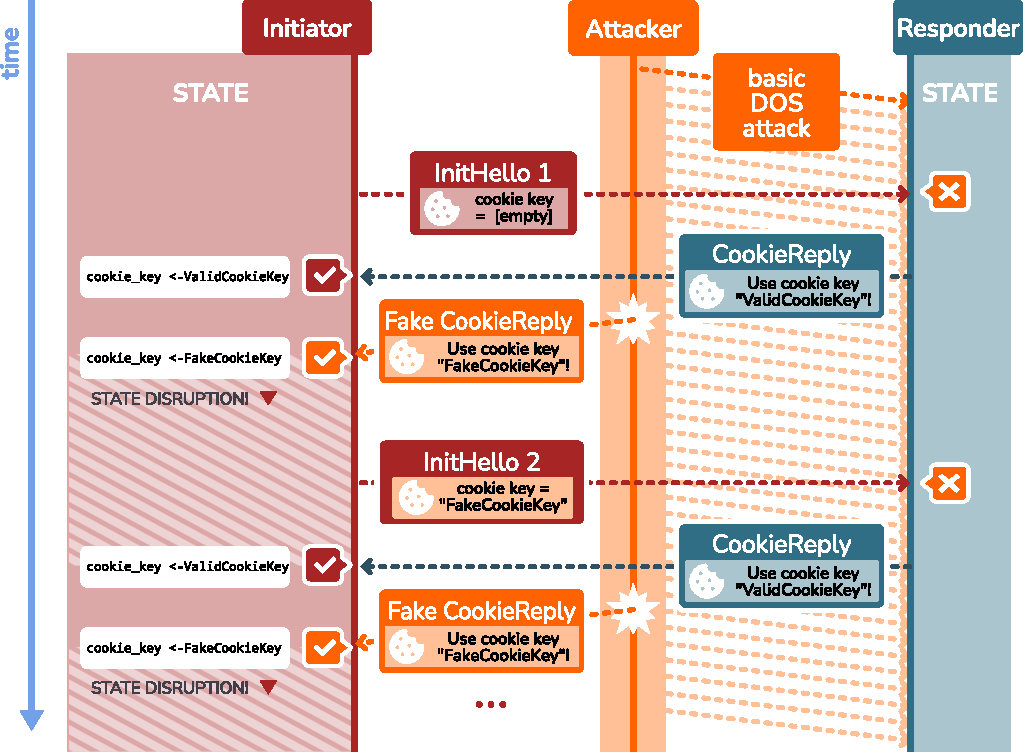
\includegraphics[height=.85\textheight]{graphics/cookiecutter-bare}
      \end{column}
      \begin{column}{.4\linewidth}
      \small
      \only<.|handout:.>{
      	\vspace{-\ht\strutbox}
          \begin{enumerate}
            \item \textbf{Attacker} begins continuous DOS attack against responder
            \item \textbf{Initiator} begins handshake, sends \emph{InitHello}
            \item \textbf{Responder} replies with \emph{CookieReply}
              \blockquote{\textbf{CookieReply:} I am under load. Prove you are not using an IP spoofing attack with this \emph{cookie key}.}
            \item \textbf{Initiator} Initiator stores cookie key and waits for their retransmission timer
            \item \textbf{Attacker} forges a cookie reply with a fake \emph{cookie key}
            \item \textbf{Initiator} Initiator overwrites the valid cookie key with the fake one
            \item[…] Repeat ad nauseam
          \end{enumerate}
      }

        \only<+|handout:+>{%
          \vspace{-\ht\strutbox}\begin{block}{Attacker gains:}
          \begin{itemize}
            \item Cheap protocol-level DOS
          \end{itemize}
          \unskip
          \end{block}
          \begin{block}{Attacker needs:}
          \begin{itemize}
            \item Knowledge of public keys
            \item Good timing 
          \end{itemize}
          \unskip
          \end{block}
          \begin{block}{Role switching:}
          \begin{itemize}
            \item WireGuard sometimes uses role switching
            \item To account for that, the attack can be performed against both peers 
          \end{itemize}
          \unskip
          \end{block}
        }
      \end{column}
    \end{columns}
\end{frame}

\begin{frame}{CookieCutter: Post-Quantum WG \& Rosenpass}
  \begin{columns}[fullwidth,T]
    \begin{column}{.6\linewidth}
      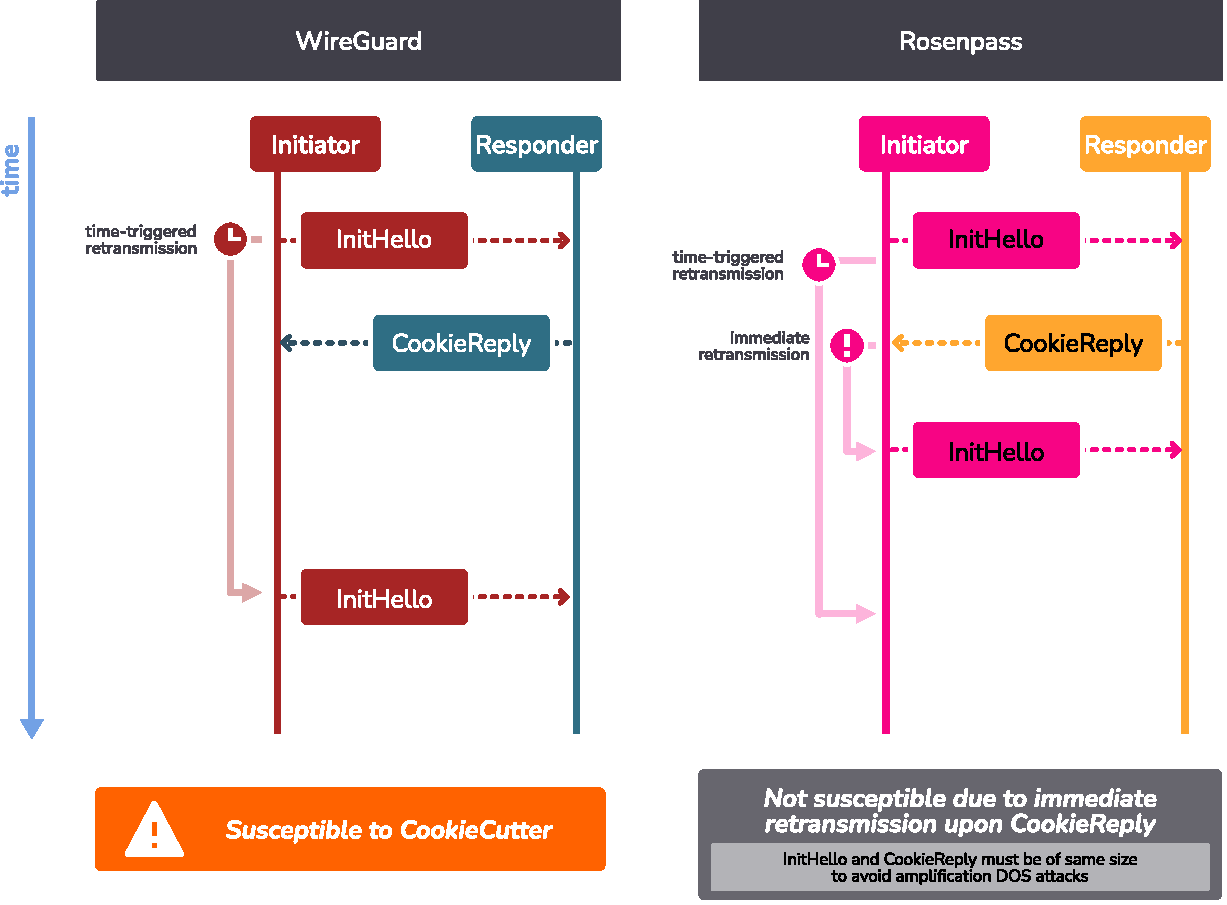
\includegraphics[keepaspectratio,height=.85\textheight]{graphics/cookiecutter-compare.pdf}
    \end{column}

    \begin{column}{.4\linewidth}
      \begin{block}{Post-Quantum WireGuard}
      \begin{itemize}
        \item No change.
      \end{itemize}
      \end{block}

      \begin{block}{Rosenpass}
      \begin{itemize}
        \item Immediate retransmission of \emph{InitHello} upon receiving \emph{CookieReply}
        \item \emph{CookieReply} and \emph{InitHello} must be of same size to prevent DOS amplication attacks
        \item[$\Rightarrow$] Rosenpass is protected from CookieCutter attacks
      \end{itemize}
      \end{block}
    \end{column}
  \end{columns}
\end{frame}

% \begin{frame}{CookieCutter: Post-Quantum WireGuard}
%   \begin{columns}[c]
%     \begin{column}{.4\textwidth}
%       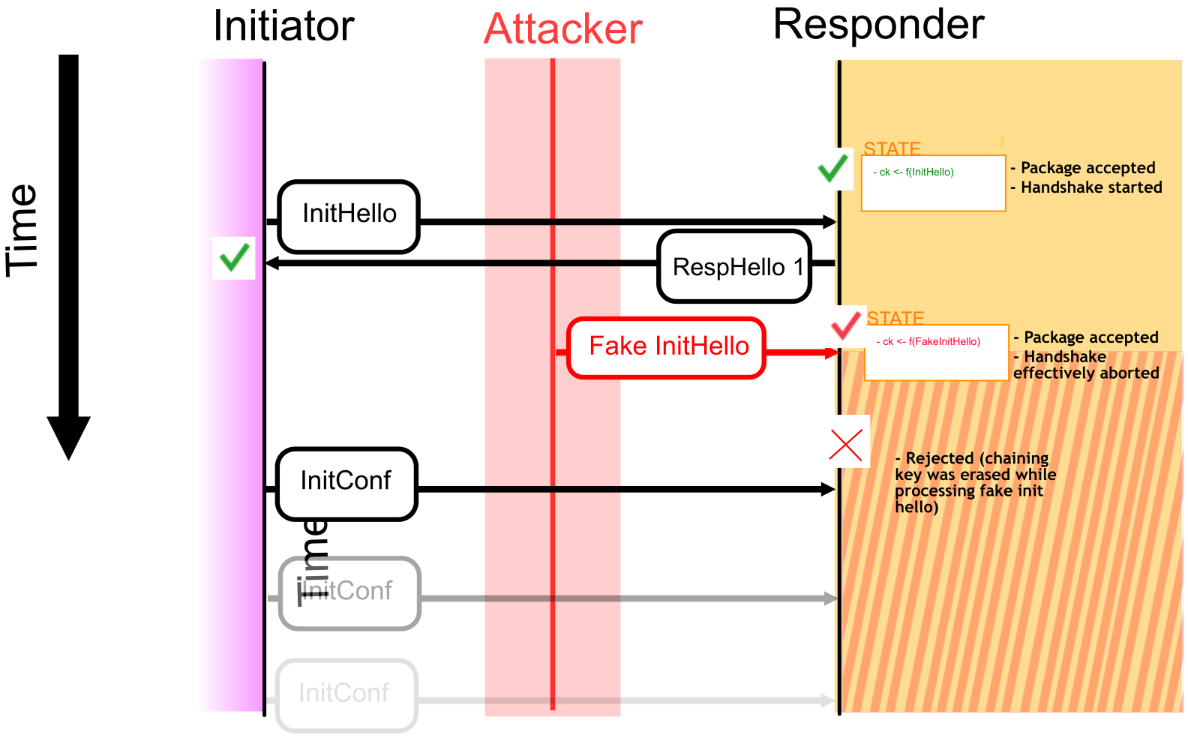
\includegraphics[keepaspectratio,width=.9\textwidth]{graphics/pqwg-state-disrupt.png}
%     \end{column}

%     \begin{column}{.6\textwidth}

%       \begin{itemize}
%       \item
%         State Disruption of Post-Quantum WireGuard is simple forgery
%         \begin{itemize}
%         \item
%           Or replay attack (if public keys are not known)
%         \end{itemize}
%       \item
%         ChronoTrigger attack still works (no NTP access needed if public keys
%         are known)
%       \end{itemize}
%     \end{column}
%   \end{columns}
% \end{frame}

% \begin{frame}{CookieCutter: Post-Quantum WireGuard and Rosenpass}
% \hypertarget{post-quantum-wireguard-and-rosenpass}{}
%   \begin{columns}[c]
%     \begin{column}{.4\textwidth}
%       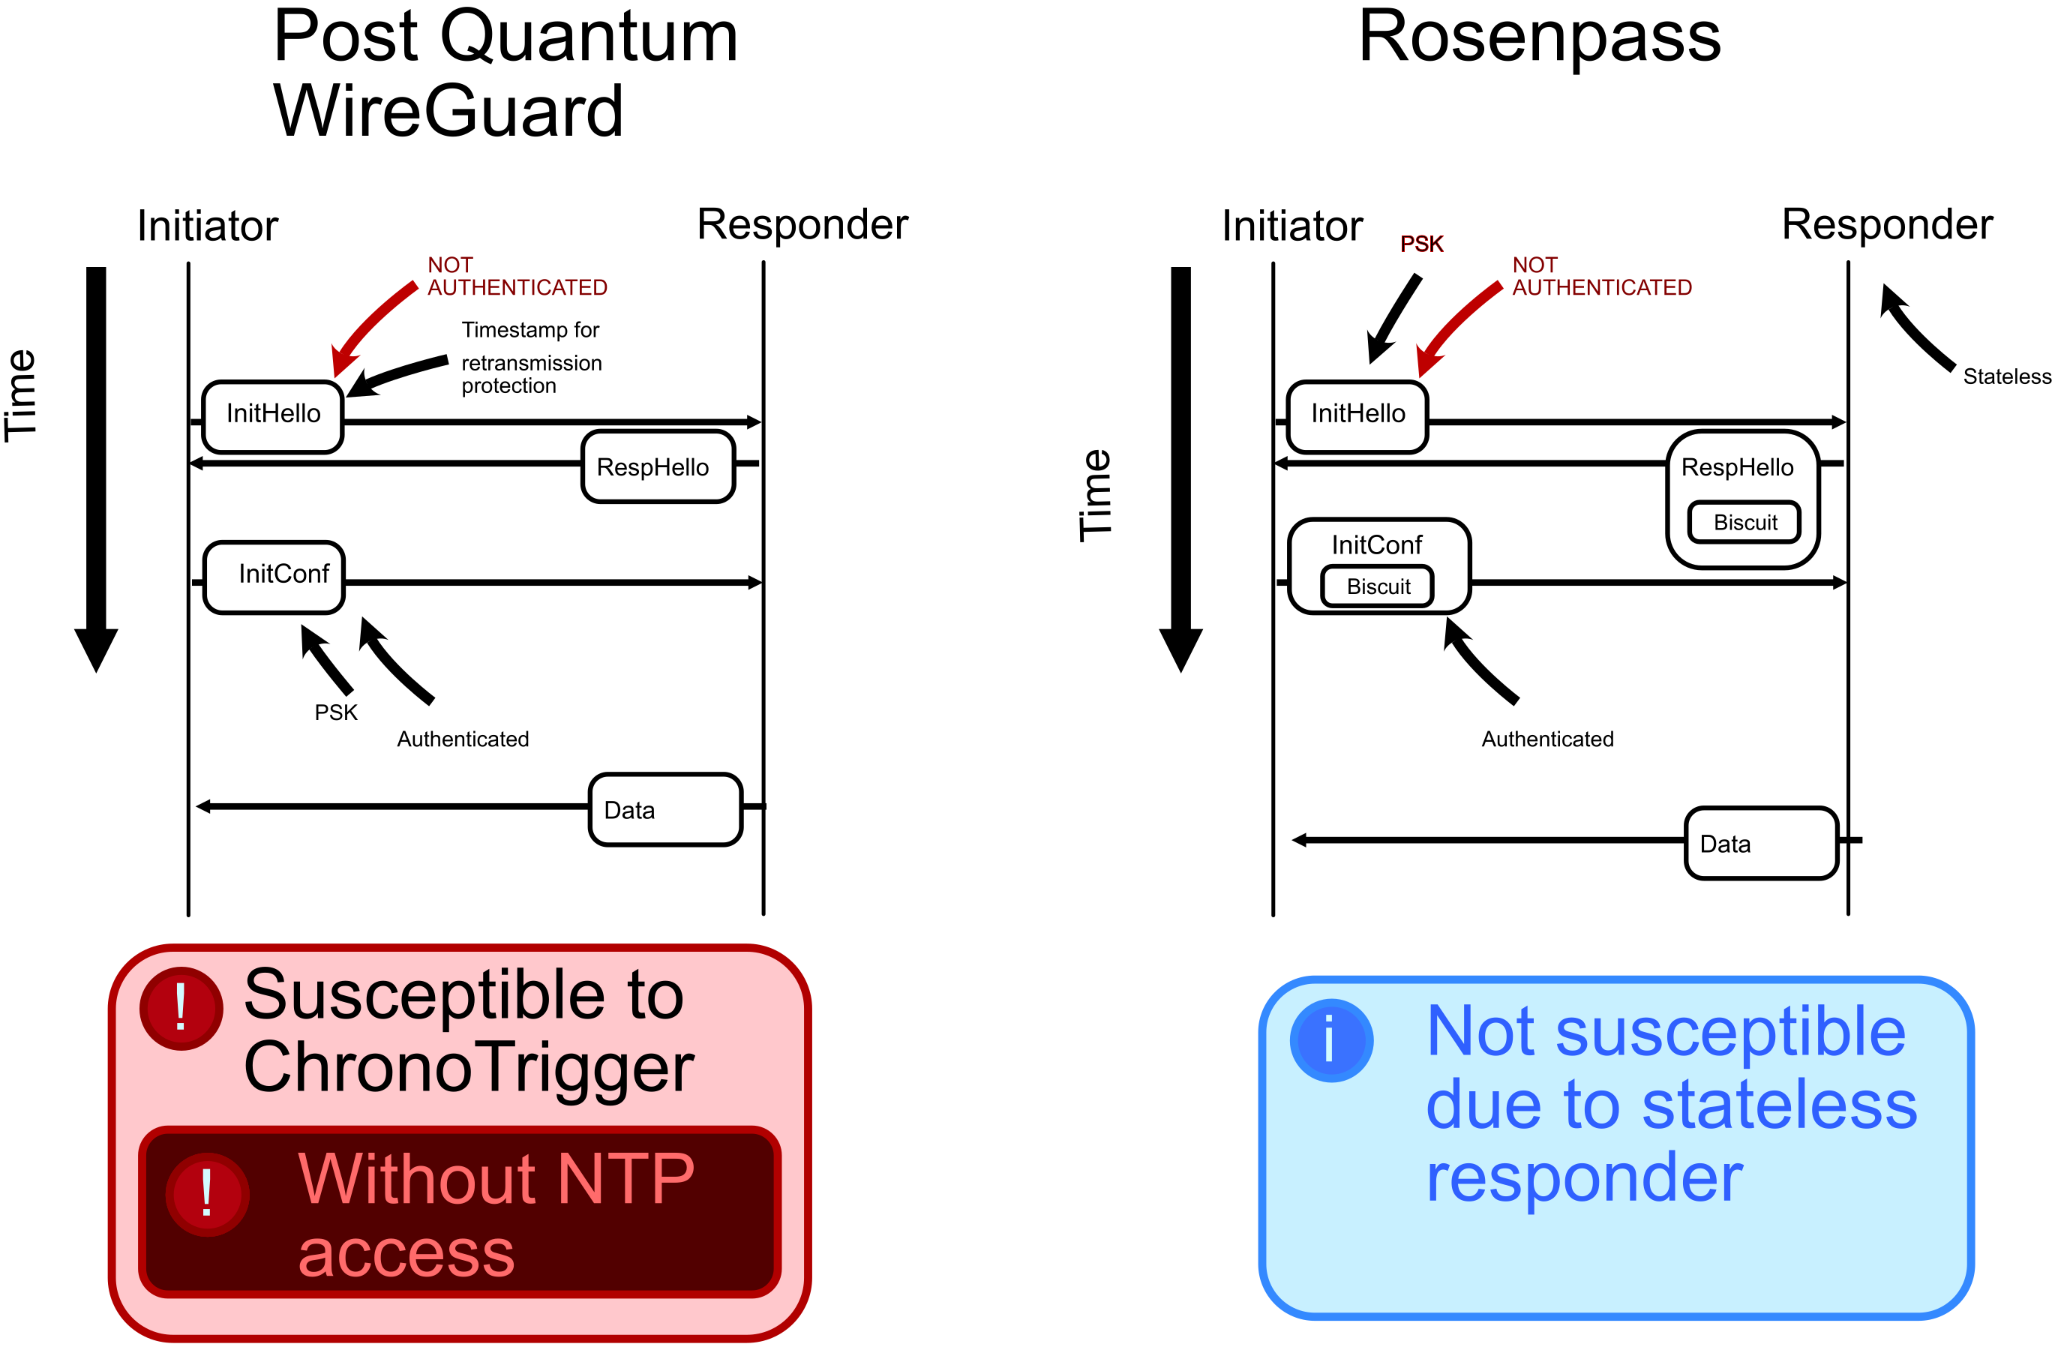
\includegraphics[keepaspectratio,width=.9\textwidth]{graphics/pqwg-rosenpass-compare.png}
%     \end{column}

%     \begin{column}{.6\textwidth}
%       \begin{itemize}
%       \item Moved PSK into (only) InitHello
%       \item
%         Stateless responder to prevent state disruption

%         \begin{itemize}
%         \item
%           State moved into biscuit
%         \end{itemize}
%       \item
%         InitHello immediately retransmitted upon CookieReply reception

%         \begin{itemize}
%         \item
%           CookieReply must be as big as InitHello to avoid amplification
%           attacks
%         \end{itemize}
%       \end{itemize}
%     \end{column}
%   \end{columns}
% \end{frame}


% \begin{frame}{ChronoTrigger Protocol Comparison}
% \hypertarget{chronotrigger-protocol-comparison}{}
% % :information\_source: (done) Dedicated scientific illustration

% % TODO(marei) see line below
% % :information\_source: Resize illustrations to make room for points

%   \begin{columns}[c]
%     \begin{column}{.4\textwidth}
%       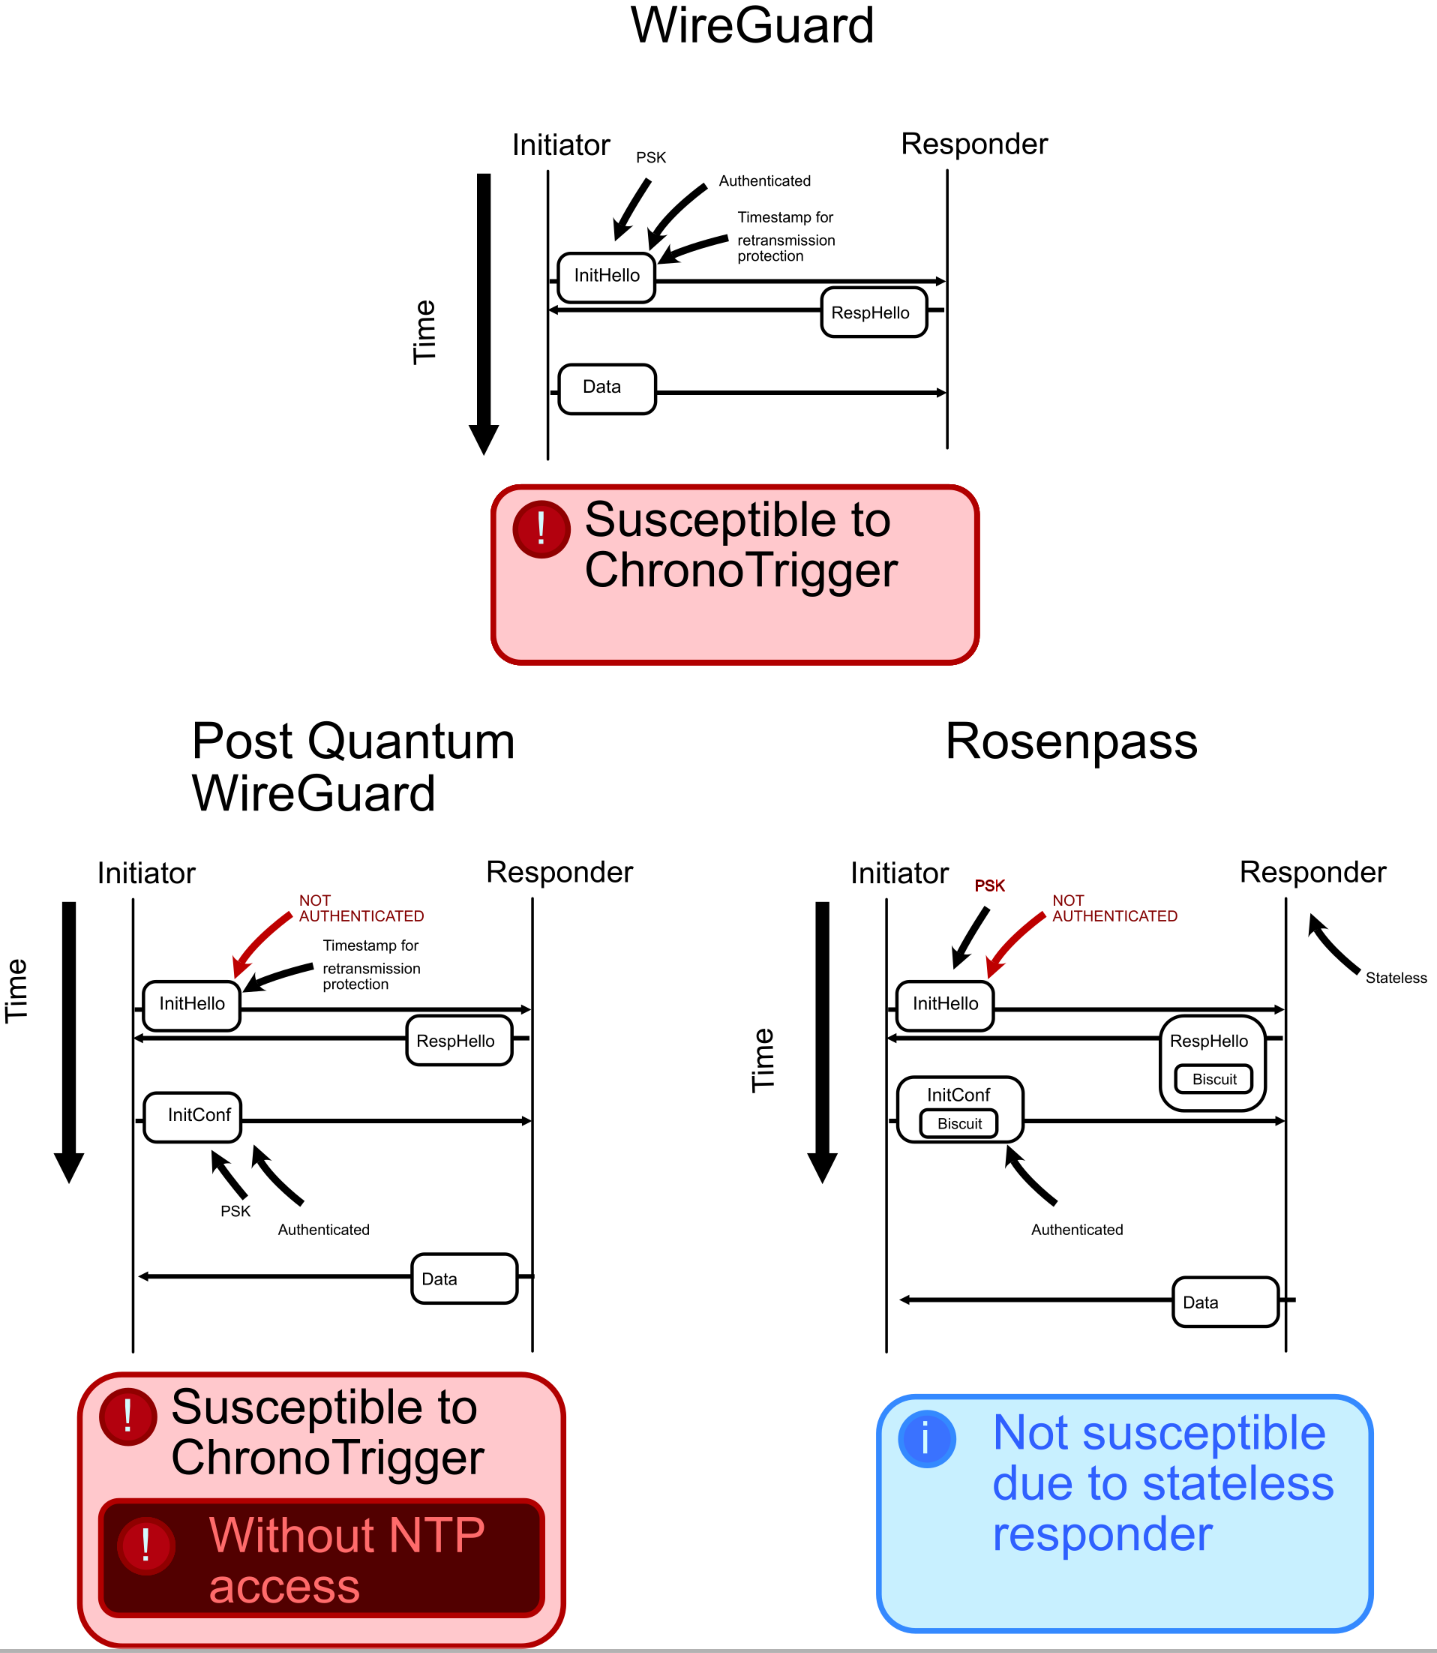
\includegraphics[keepaspectratio,width=.9\textwidth]{graphics/chronotrigger-compare.png}
%     \end{column}

%     \begin{column}{.6\textwidth}
%       \begin{itemize}
%       \item
%         WireGuard: Affected
%       \item
%         Post-Quantum WireGuard: Worse (public key knowledge is sufficient for
%         kill token generation)
%       \item
%         Rosenpass: Secured by being stateless
%       \end{itemize}
%     \end{column}
%   \end{columns}
% \end{frame}

% \begin{frame}{CookieCutter Protocol Comparison}
% % :information\_source: (done) Dedicated scientific illustration

% % TODO(marei) see line below
% % :information\_source: Resize illustrations to make room for points

%   \begin{columns}[c]
%     \begin{column}{.4\textwidth}
%       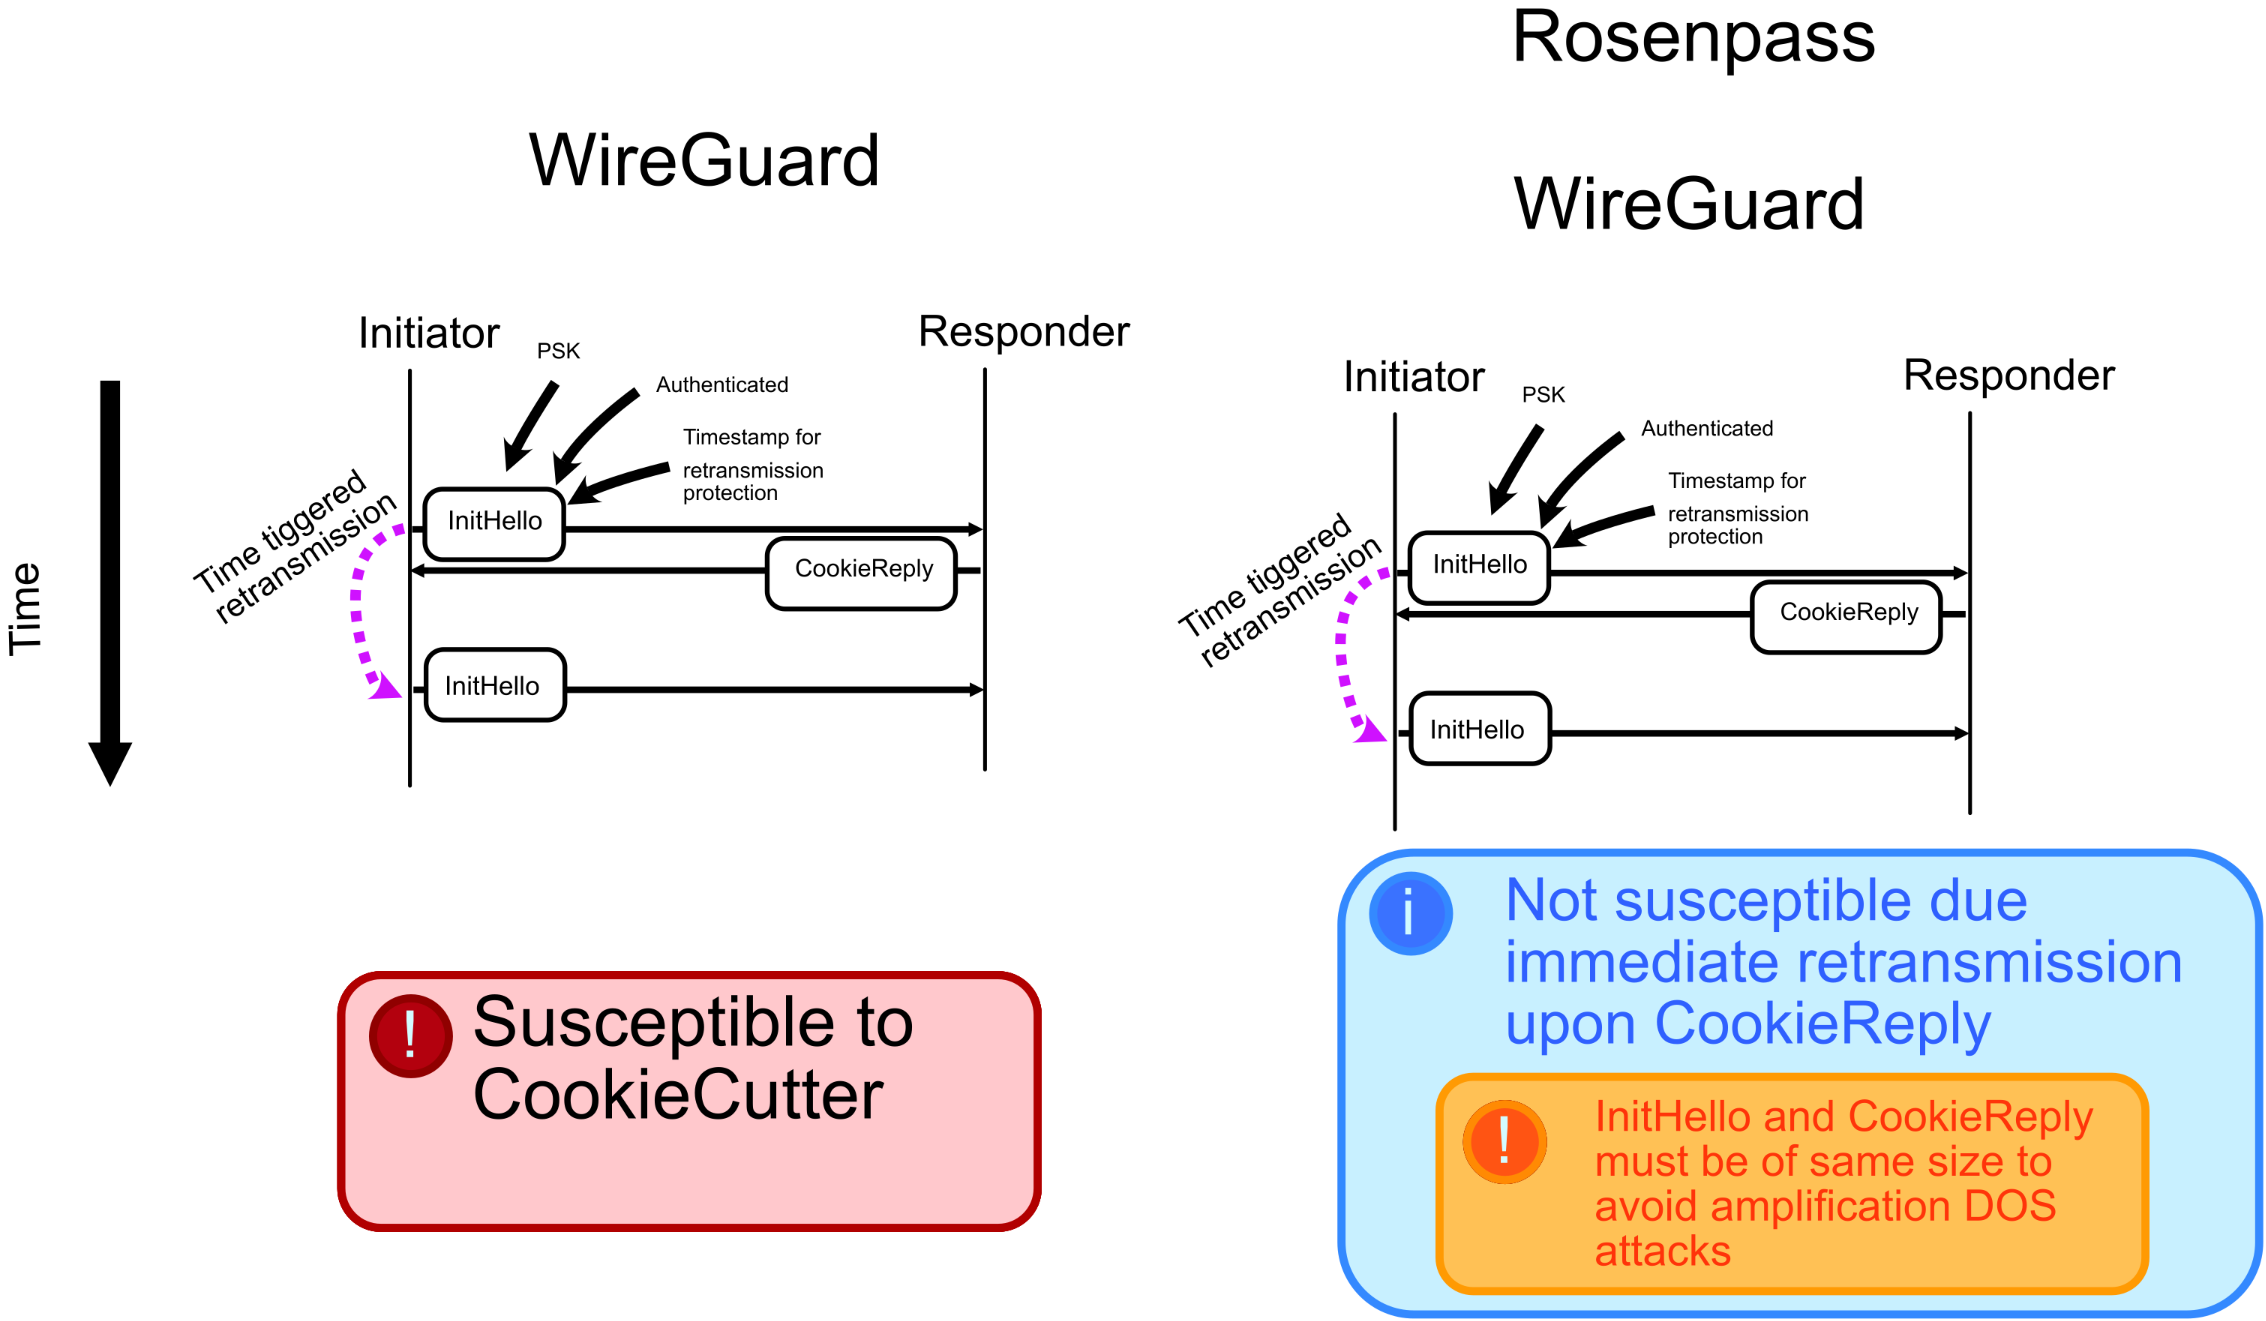
\includegraphics[keepaspectratio,width=.9\textwidth]{graphics/cookiecutter-compare.png}
%     \end{column}

%     \begin{column}{.6\textwidth}
%       \begin{itemize}
%       \item
%         WireGuard: Affected
%       \item
%         Post-Quantum WireGuard: Affected
%       \item
%         Rosenpass: Unaffected by immediate retransmission of InitHello upon
%         CookieReply receipt

%         \begin{itemize}
%         \item
%           (CookieReply and InitHello must be of same size)
%         \end{itemize}
%       \end{itemize}
%     \end{column}
%   \end{columns}
% \end{frame}

\interlude[4]<Trials \textasciitilde\ Advanced Security Properties>{Knock Patterns}

\begin{frame}{Rosenpass and WireGuard: Advanced Security}
\hypertarget{wireguard-advanced-security-properties}{}
\vspace*{-\baselineskip}
\small
\begin{columns}[fullwidth,T]
	\setlength\leftmargini{\labelwidth+\labelsep}
  \begin{column}{.48\linewidth}
% TODO(marei): Can we make the smilies look nicer
    \begin{block}{\strut CPU DOS mitigation:}
    \begin{itemize}
      \item No change on the protocol level.
      \item[{\Sey[][green!60!white]} ] Slightly worsened in practice because PQ operations are more expensive than elliptic curves
    \end{itemize}
        \unskip
    \end{block}
    \begin{block}{\strut Limited Stealth:}
    \begin{itemize}
      \item No change in Rosenpass, but we should have \textbf{full stealth}!
      \item[$\Rightarrow$] Remove cookie mechanism?
      \item[{\Sey[][green!60!white]} ] This would affect the CPU DOS mitigation too much.
    \end{itemize}
    \unskip
    \end{block}

  \end{column}

  \begin{column}{.48\linewidth}
    \begin{block}{\strut Limited Identity Hiding:}
    \begin{itemize}
      \item No change in Rosenpass, but we should have \textbf{full identity hiding}!
      \item[$\Rightarrow$] Do not use pre-authentication with public key?
      \item[{\Sey[][green!60!white]} ] This would affect the CPU DOS mitigation, possibly too much.
    \end{itemize}
        \unskip
    \end{block}
    % \textbf{Interruption resistance:} \vspace{0.5em} % TODO(blipp): Mark red somehow?
    % \begin{itemize}
    %   \item[ {\Laughey[1.4]} ] supported and modeled!
    % \end{itemize}
  \end{column}
\end{columns}
\end{frame}

% \begin{frame}{Rosenpass Advanced Security Properties}
% \hypertarget{rosenpass-advanced-security-properties}{}
% % :information\_source: (done) Insert protocol time diagram on left side

%   \begin{columns}[c]
%     \begin{column}{.4\textwidth}
%       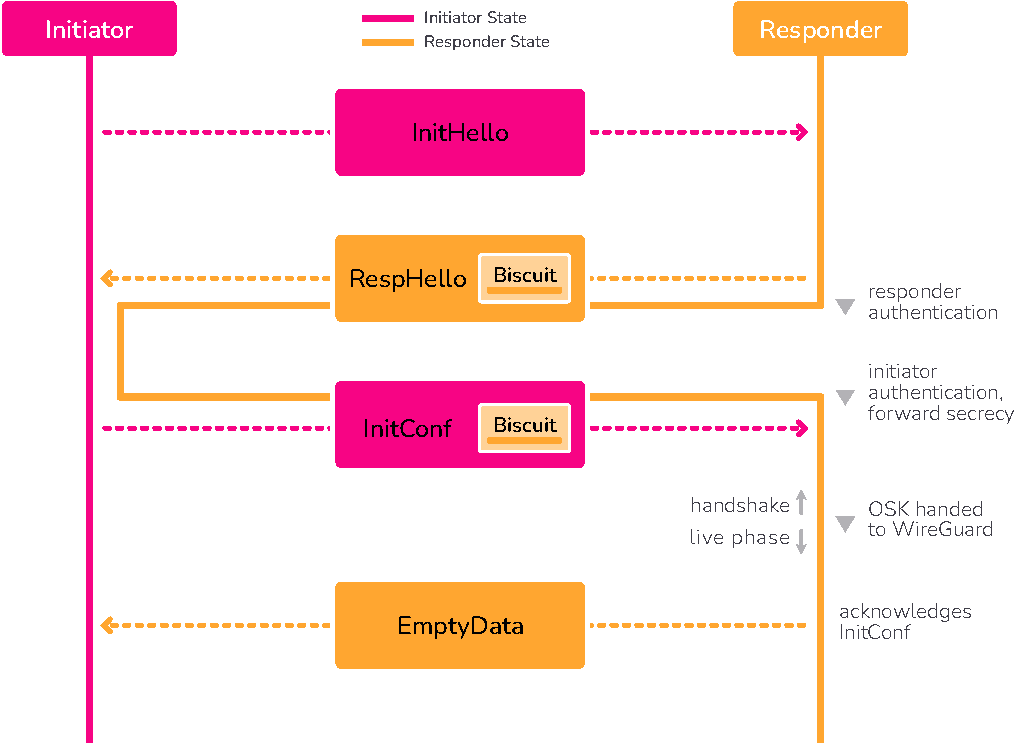
\includegraphics[keepaspectratio,width=.9\textwidth]{graphics/rosenpass-wp-key-exchange-protocol-rgb.pdf}
%     \end{column}

%     \begin{column}{.6\textwidth}
%       \only<1>{
%         \textbf{Limited Stealth:}

%         \begin{itemize}
%         \item
%           Protocol should not respond to packages without some
%           pre-authentication
%         \item
%           Proof of IP ownership (cookie mechanism) prevents full stealth
%         \item
%           Attacker needs to know responder key
%         \item
%           Full stealth needs initiator authentication in first package
%         \end{itemize}
%       }

%       \only<1-2>{
%         \textbf{Limited Identity Hiding:}

%         \begin{itemize}
%         \item
%           Attacker can guess identities due to use in the MAC in the auth code
%         \end{itemize}
%       }

%       \only<2-3>{
%         \textbf{Limited CPU DOS protection:}

%         \begin{itemize}
%         \item
%           Preventing CPU-exhaustion DOS involving network amplification
%           attacks
%         \item
%           Proof of IP ownership
%         \item
%           \textbf{Slightly more exposed due to more expensive cryptographic
%           operations}
%         \end{itemize}
%       }
%       
%       \only<3>{
%         \textbf{Full interruption (state disruption) resistance:} Stateless
%         responder

%         \textbf{Post-Quantum secure!}
%       }

%       \only<4>{
%       $\Rightarrow$
%         Rosenpass is as secure as WireGuard but using
%         PostQuantum security

%       $\Rightarrow$
%         Additional state disruption resistance

%       $\Rightarrow$
%         CPU-exhaustion resistance is slightly worse, but that
%         is due to the cost of the cryptographic primitives
%       }
%     \end{column}
%   \end{columns}
% \end{frame}

\begin{frame}{Choose Two: Stealth, Identity Hiding, CPU DOS Mit.}
  \centering
  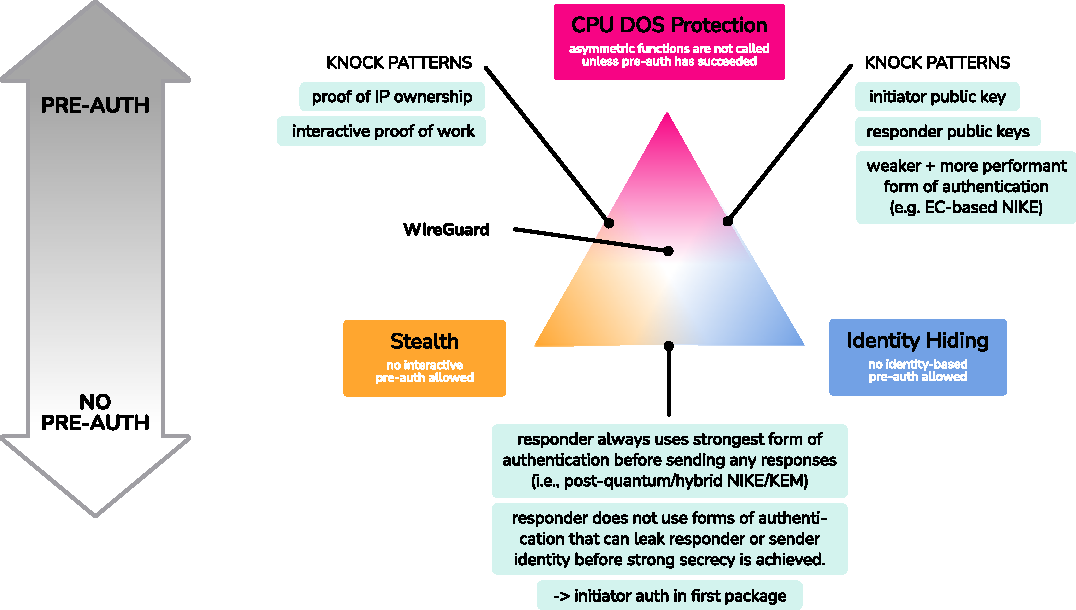
\includegraphics[height=.85\textheight]{graphics/preauth-tradeoff-bare.pdf}
\pdfpcnote{Stealth + Identity Hiding\\
* Disable pre-auth with public key in symmetric MAC\\
* Disable cookie-mechanism\\
* => No CPU DOS mitigation\\
\\
Stealth + CPU DOS mitig.\\
* Disable cookie-mechanism\\
* => Limited identity hiding due to public key in symmetric MAC\\
\\
Identity hiding + CPU DOS mitig.\\
* Disable pre-auth with public key in symmetric MAC\\
* => Limited stealth due to cookie mechanism
}
\end{frame}

%\begin{frame}{Choose Two: Stealth, Identity Hiding, CPU DOS Mit.}
%\begin{columns}[fullwidth,T]
%\begin{column}{.53\linewidth}
%\begin{overlayarea}{\linewidth}{ .85\textheight}
%\vfill
%\raisebox{-.5\height}{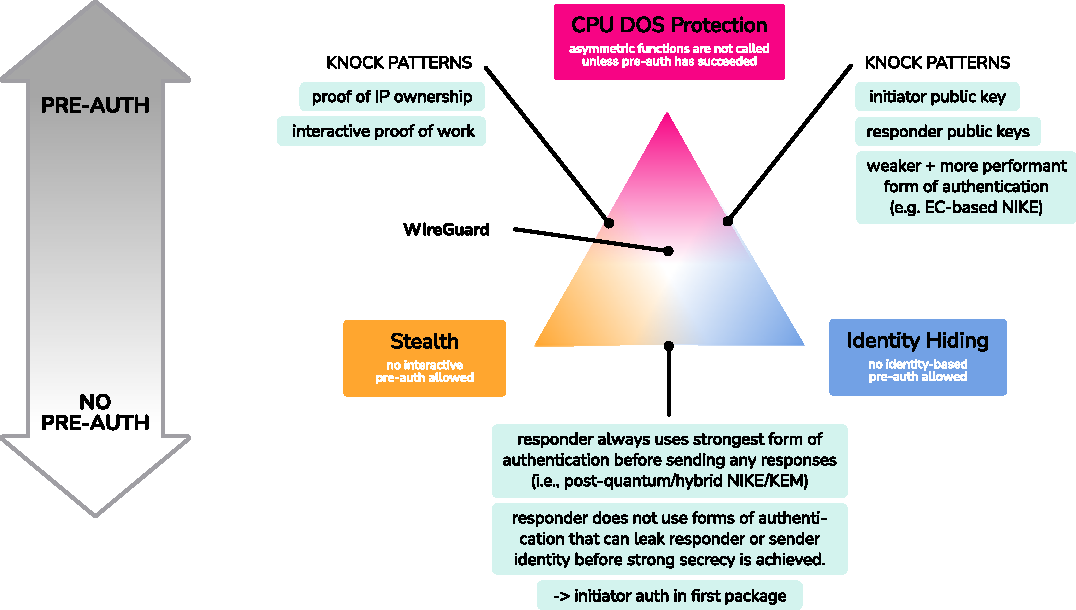
\includegraphics[width=\linewidth]{graphics/preauth-tradeoff-bare.pdf}}
%\par
%\vfill
%  \end{overlayarea}
%\end{column}%
%    \begin{column}{.45\linewidth}
%    \small
%      \begin{enumblock*}{Stealth + Identity Hiding:}
%      \only<+>{
%      \begin{itemize}
%        \item Disable pre-auth with public key in symmetric MAC
%        \item Disable cookie-mechanism
%        \item[$\Rightarrow$] No CPU DOS mitigation
%      \end{itemize}
%      \unskip}
%      \end{enumblock*}
%      \begin{enumblock*}{Stealth + CPU DOS mitig.:}
%      \only<+>{
%      \begin{itemize}
%        \item Disable cookie-mechanism
%        \item[$\Rightarrow$] Limited identity hiding due to public key in symmetric MAC
%      \end{itemize}
%      \unskip}
%      \end{enumblock*}
%      \begin{enumblock*}{Identity hiding + CPU DOS mitig.:}
%    \only<+>{
%      \begin{itemize}
%        \item Disable pre-auth with public key in symmetric MAC
%        \item[$\Rightarrow$] Limited stealth due to cookie mechanism
%      \end{itemize}
%      \unskip}
%      \end{enumblock*}
%    \end{column}
%\end{columns}
%\end{frame}

\begin{frame}{WireGuard and Rosenpass Trade-Offs}
  \begin{columns}[fullwidth,T]
\begin{column}{.53\linewidth}
\begin{overlayarea}{\linewidth}{ .85\textheight}
\vfill
\raisebox{-.5\height}{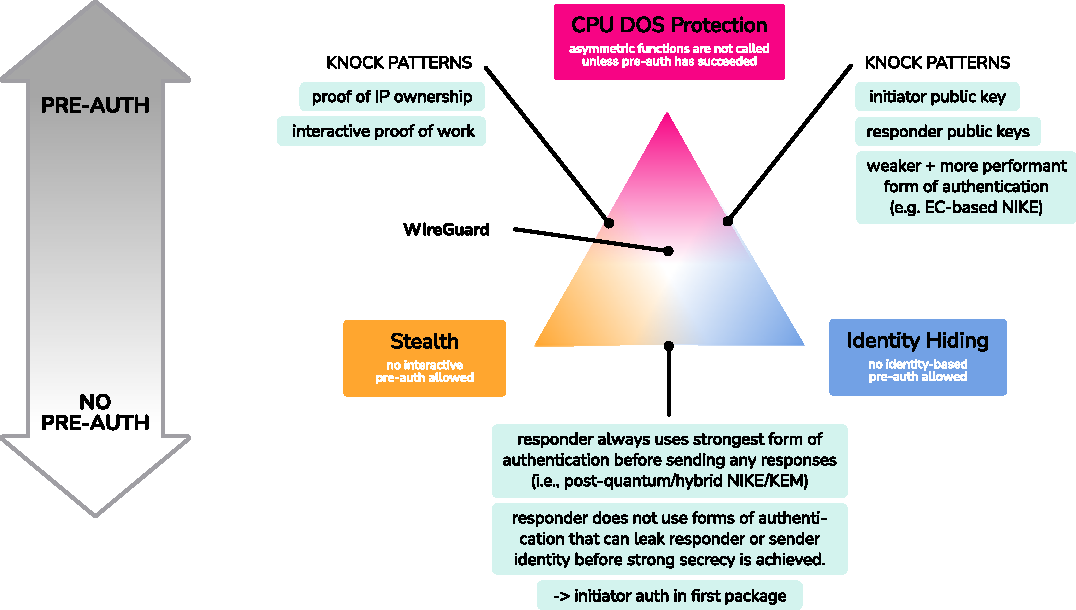
\includegraphics[width=\linewidth]{graphics/preauth-tradeoff-bare.pdf}}
\par
\vfill
\end{overlayarea}
\end{column}
    \begin{column}{.45\linewidth}
    \small
      \begin{block}{CPU DOS Mitigation:}
      \only<+|handout:+>{
      \begin{itemize}
        \item There is no clear optimum here.
        \item CPU DOS mitigation is never calling asymmetric crypto unless we know it succeeds (circular reasoning)
      \end{itemize}
      \unskip
      }
      \end{block}
       \begin{block}{Stealth:\vphantom{g}}
      \only<+|handout:+>{
      \begin{itemize}
        \item Broken on DOS attacks assuming recipient is known % TODO(blipp): Fact check
        \item[$\Rightarrow$] This seems acceptable
      \end{itemize}
      \unskip
      }
      \end{block}
    \begin{block}{Identity hiding:}
     \only<+|handout:+>{
      \begin{itemize}
        \item Broken on knowledge of public keys
        \item[$\Rightarrow$] This seems inacceptable!
        \item[$\Rightarrow$] Investigate proper identity hiding without overly impacting stealth and CPU DOS mitig.
      \end{itemize}
      \unskip
      }
      \end{block}
    \end{column}
  \end{columns}
\end{frame}

\begin{frame}{Knock Patterns}
\begin{columns}[fullwidth,c]
    \begin{column}{.45\linewidth}
    \rlap{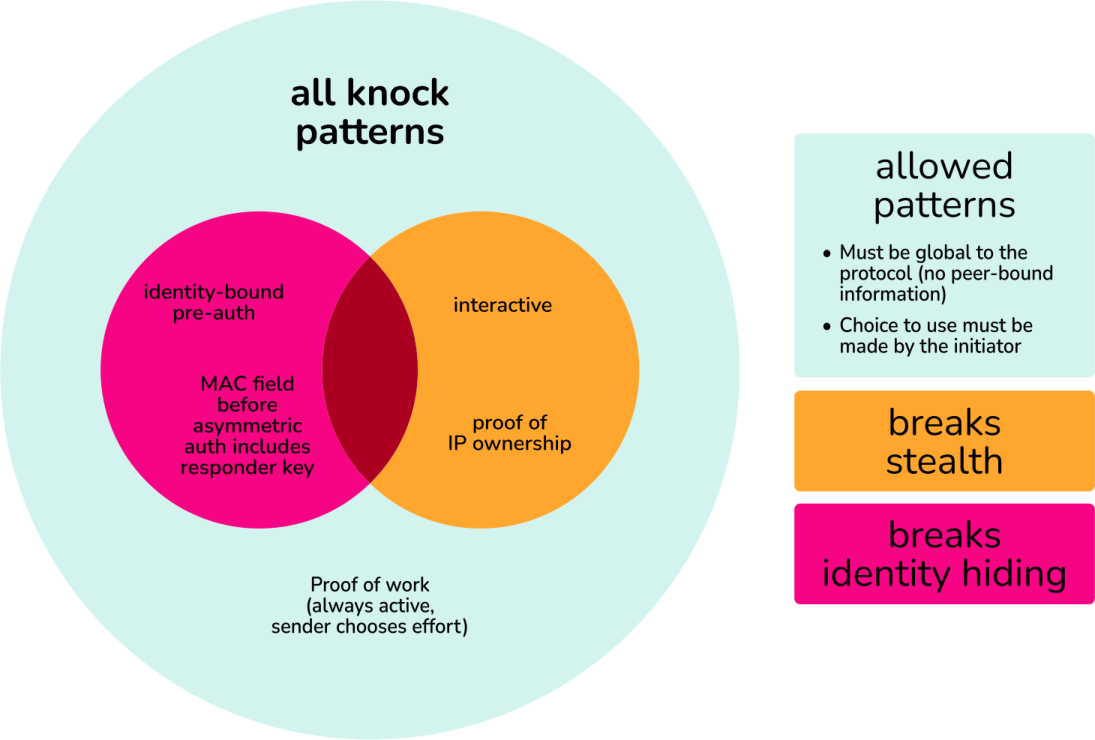
\includegraphics[keepaspectratio,width=\linewidth]{graphics/knock-patterns-bare.pdf}}
    \end{column}%
    \begin{column}{.5\linewidth}
      \begin{itemize}
        \item We choose to think of WireGuard's and Rosenpass' pre-auth as \say{Knock Patterns}
        \item These knock patterns have severe trade-offs.
        \item Interactive knock pattern (cookie mechanism) breaks stealth
        \item Identity-based knock patterns (e.g., knowledge of public key) breaks identity hiding
        \vspace{0.5em}
        \item[$\Rightarrow$] Avoid identity-bound knock patterns
        \item[$\Rightarrow$] Minimize interactive knock patterns
        \item[$\Rightarrow$] Explore other (allowed) knock patterns
      \end{itemize}
    \end{column}
  \end{columns}
\end{frame}


\begin{frame}{Tools to the Table!}
Bellare and Rogaway [BR06], Halevi [Hal05]:\\
\hspace{1.618em} Call for “automated tools, that can help write and verify game-based proofs”\\[1.618em]
%
\visible<2->{%
Do the tools \emph{actually help}? And if yes, whom?\\[1.618em]

ProVerif, Tamarin, CryptoVerif, EasyCrypt:\\
\hspace{1.618em} We like these tools, they are good!\\[1.618em]%
}
\visible<3->{%
They mostly help the \emph{formal verification experts} to:
\begin{itemize}
\item do analyses themselves, write papers
\item develop proof methodologies, foundation work for formal methods
\end{itemize}
}
% c.f. Manuel's talk about EasyCrypt
\end{frame}




%\begin{frame}{Pen and Paper proofs}
%\hypertarget{pen-and-paper-proofs}{}
%
%% Karo talk:
%% * proof should be part of the engineering effort
%% * updating a pen-and-paper proof is a mess
%
%
%% the reasons from Joseph's talk, and
%% * pen-and-paper proofs are often read-only
%% * hard to maintain and update, especially so by other people
%% * part of engineering effort: gap to implemented systems too large?
%
%
%
%\begin{itemize}
%\item
%  Become increasingly unwieldy
%\item
%  Karolin anecdote: Recently found major issues in fairly prominent
%  paper, page N
%
%  \begin{itemize}
%  \item
%    (TODO: Handle issues found with Signal analysis)
%  \end{itemize}
%\item
%  Proof state is hard to keep track off
%\end{itemize}
%
%% :information\_source: Insert screen-shot of PostQuantum WireGuard
%% paper showing WireGuard proof differential
%\end{frame}
%
%% Issues with proof tools
%% ProVerif
%% * no syntax highlighting or other integration available in your favourite editor
%% * no good tooling for engineering at scale (e.g., macro language/preprocessor)
%% * hard to understand output and error messages
%
%
%
%
%
%\begin{frame}{ProVerif}
%\hypertarget{proverif}{}
%% :information\_source: Insert screen-shot of our ProVerif analysis
%
%% :information\_source: Cut off screen-shot of our code
%
%
%% Karo talk
%% * no syntax highlighting in Vim
%% * preprocessor to be able to split up into multiple files
%% * educated guesswork with use of some tooling, but it is opaque/undocumented
%% * 
%
%% TODO
%% * add screenshot of raw output
%% * 
%
%
%\begin{itemize}
%\item
%  No syntax highlighting
%\item
%  No good tooling to do engineering at scale (karolin resorted to the C
%  preprocessor)
%\end{itemize}
%
%% :information\_source: Insert screen-shot of raw ProVerif output on
%% the left; out colorful output on the side. \textgreater{} Big letters
%% (text below) on white superimposed on split-screen screenshot
%
%ProVerif output is not made for Humans
%\end{frame}
%
%\begin{frame}{CryptoVerif}
%\hypertarget{cryptoverif}{}
%% :information\_source: Insert screen-shot of HPKE or WG analysis by
%% blipp
%
%% :information\_source: Cut off screen-shot
%
%TODO: Blipp - Expert driven engineering
%
%% :information\_source: Insert screen-shot of CV documentation saying
%% ``to be done''
%
%% :information\_source: Cut off screen-shot
%
%\begin{itemize}
%\item
%  Sometimes the information is simply lacking
%\item Automation focused
%\item Always operating on the entire proof state
%\item complete lack of tooling
%\end{itemize}
%
%% TODO screenshot CV manual “we will add some things here”
%% * screenshot game state, maybe HPKE
%
%
%\end{frame}
%
%\begin{frame}{Tamarin}
%\hypertarget{tamarin}{}
%% :information\_source: Insert screen-shot of horn clause in text
%
%\begin{itemize}
%\item
%  When we evaluated Tamarin for use in Rosenpass you had to directly
%  encode horn clauses
%\item
%  There are new frontends there now
%\item
%  This is the prover we know least about (looking for input!)
%\end{itemize}
%\end{frame}
%
%\begin{frame}{EasyCrypt}
%\hypertarget{easycrypt}{}
%% :information\_source: Insert screen-shot of nice EC code
%
%\begin{itemize}
%\item
%  This appears to be the most complete approach right now
%\item
%  Writing proofs is hard
%\item
%  No demonstration of use with protocols at the moment
%\item
%  Anecdote:
%
%  \begin{itemize}
%  \item
%    When we tried out EC we asked advanced EC researchers at MPI-SP for
%    a tutorial to look at
%  \item
%    The tutorial contained an unknown syntax
%  \item
%    We where trying to figure out what this did
%  \item
%    I went to the very advanced researchers
%  \item
%    They thanked me for the interruption and started reverse engineering
%    the tool because they did not know either
%  \item
%    =\textgreater{} Engineering problem ``naturally-grown'' code bases
%  \end{itemize}
%\end{itemize}
%\end{frame}
%
%\begin{frame}{Protocol proof approaches}
%\hypertarget{protocol-proof-approaches}{}
%\begin{itemize}
%\item
%  Pen and paper proofs are hard to vet and error prone
%
%  \begin{itemize}
%  \item
%    Provide a lot of flexibility, this is a good thing
%  \end{itemize}
%\item
%  Formal verification tools work, but they are hard to use.
%
%  \begin{itemize}
%  \item
%    THEY ARE ALSO HARD TO READ EVEN FOR THE AUTHORS
%  \end{itemize}
%\item
%  Option: The basic models may be there
%
%  \begin{itemize}
%  \item
%    They are very strict and formally correct
%  \end{itemize}
%\item
%  We need more ability to hand-wave in formal methods proofs
%
%  \begin{itemize}
%  \item
%    This is supposed to make proofs easier; it is an incremental process
%  \end{itemize}
%\item
%  We need to improve tooling
%
%  \begin{itemize}
%  \item
%    More tooling (syntax highlighting, interactive proof assistants)
%  \item
%    More user experience (understandable output from proof verifcation
%    tools)
%  \item
%    More expressiveness
%  \end{itemize}
%\end{itemize}
%\end{frame}
%
%\begin{frame}{Protocol proof approaches}
%\hypertarget{protocol-proof-approaches-1}{}
%% :information\_source: Center text, no decorations (i.e.~no top bar),
%% big letters.
%
%More expressiveness in formal verification tools
%\end{frame}
%
%\begin{frame}{Oracle declarations in the Rosenpass ProVerif model}
%\hypertarget{oracle-declarations-in-the-rosenpass-proverif-model}{}
%% :information\_source: Screen shot of one verbose oracle declaration
%in the Rosenpass symbolic model
%
%% :information\_source: Another screenshot
%
%% :information\_source: A screenshotg of a complex C macro in tghe
%% symbolic analysis
%
%% :information\_source: A screenshotg of a proverif macro expansion in
%% ProVerif
%
%% :information\_source: White text on the right side
%
%\begin{itemize}
%\item
%  A more powerful language with native support for complex syntax sugar
%  would help a lot
%\item
%  Syntax rewriting is a basic element of proofs
%\item
%  It is suprising that our cryptographic proof tools completely lack
%  support for native syntax extensions
%\item
%  Syntax rewriting is called ``macros'' when computer-scientists do it
%\item
%  We have a tool for that; it is called lisp
%\end{itemize}
%\end{frame}


\hypertarget{section-epilogue}{%
\section{Section: Epilogue}\label{section-epilogue}}

\interlude[6]{Epilogue}

% :information_source: Add wireGuard Dragon and Bunny
\setbeamertemplate{background canvas}{\vbox to .9\paperheight {\vspace*{\fill}\transparent{.1}\makebox[\paperwidth][c]{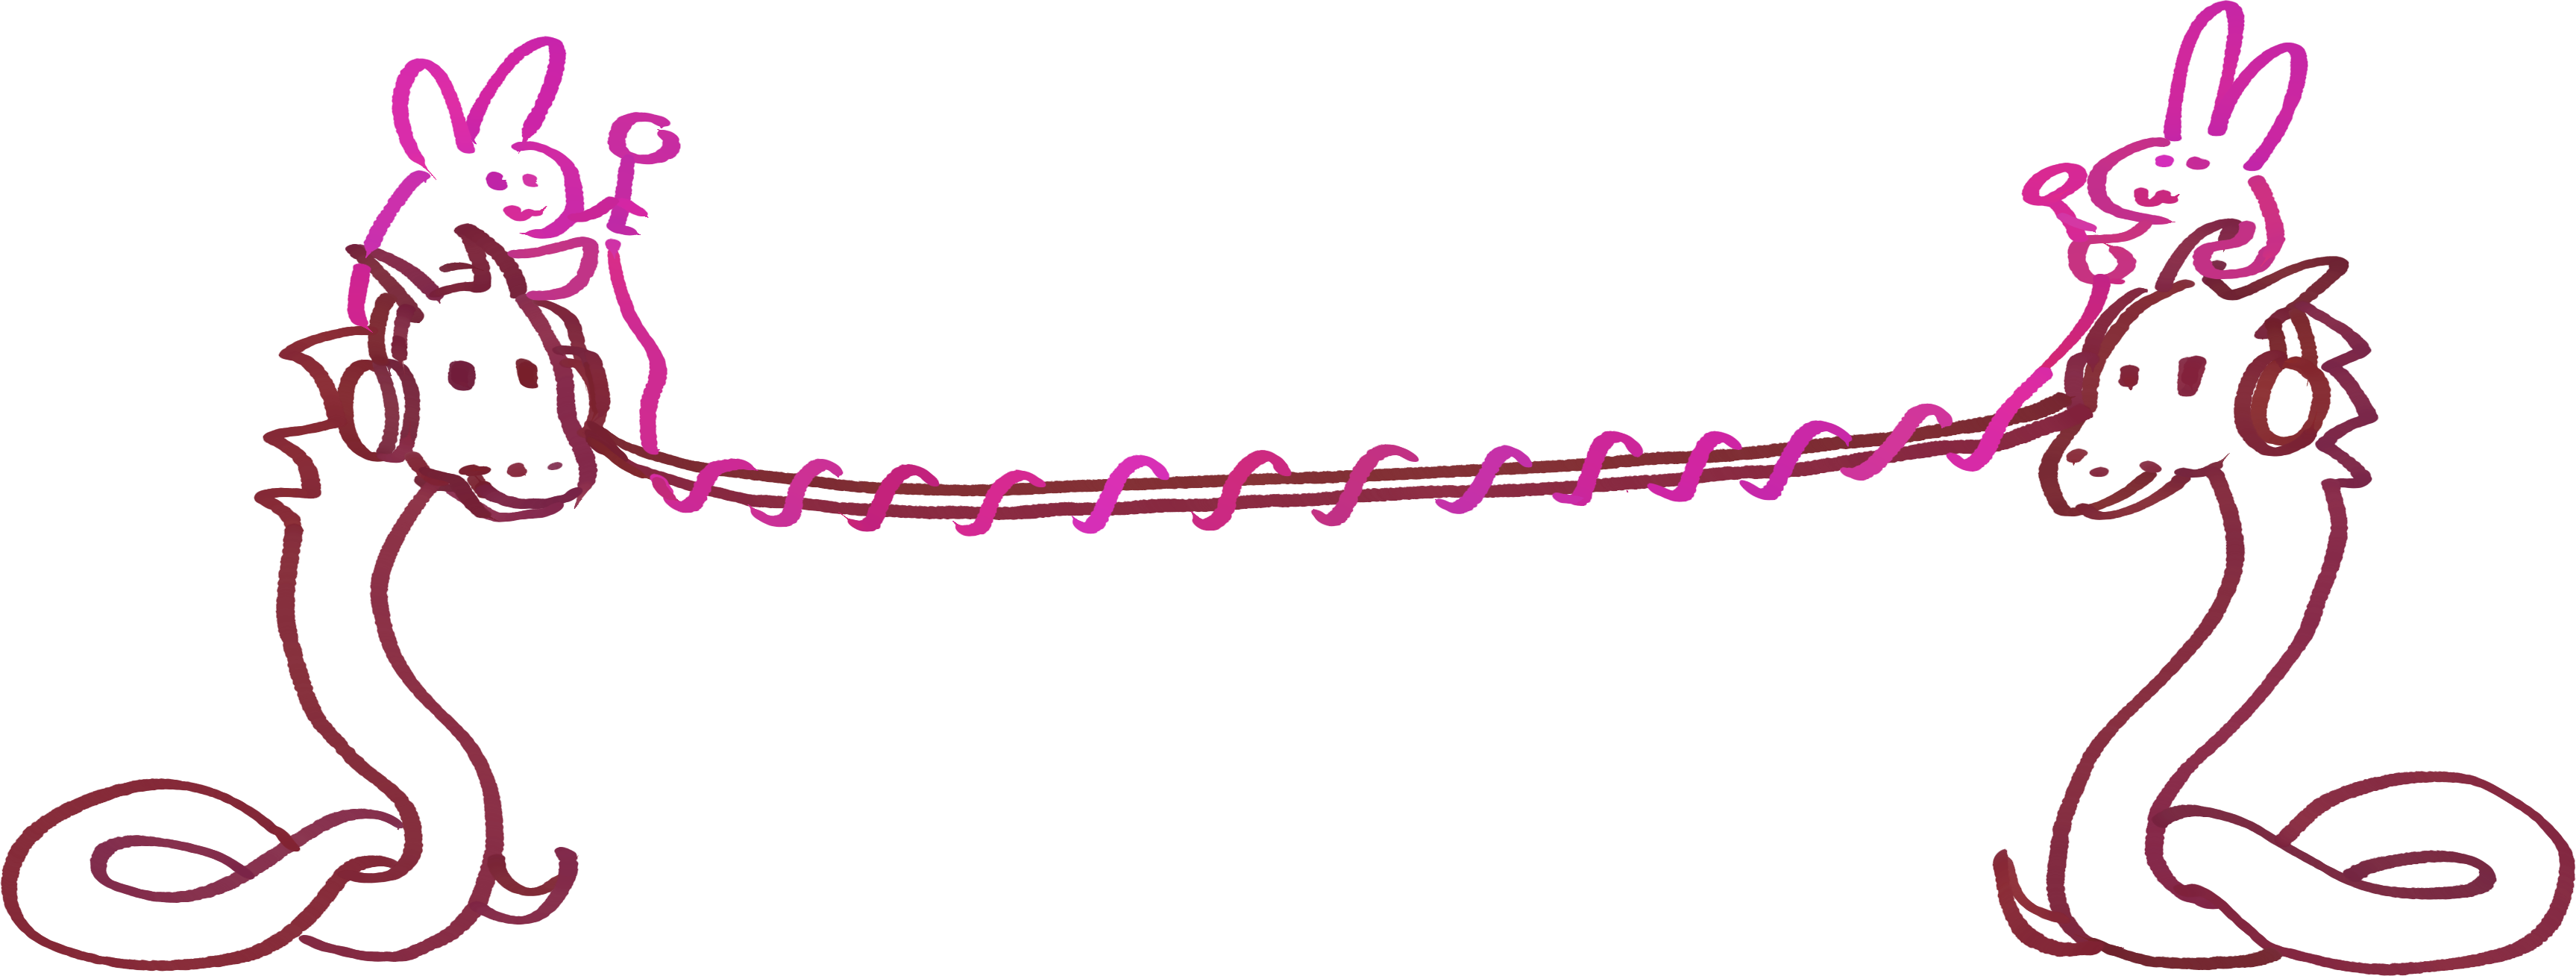
\includegraphics[width=\linewidth]{graphics/wireguard-and-rp-bunny-rose.png}}}}

\begin{frame}{Conclusion}
\hypertarget{conclusion}{}
\vspace{-\ht\strutbox}
  \begin{columns}[t]
    \begin{column}{.30\linewidth}
      \begin{block}{Rosenpass\hypertarget{rosenpass-1}{}\strut}
      \begin{itemize}
      \item
        Post-quantum secure AKE
      \item
        Same security as WireGuard
      \item
        Improved state disruption resistance
      \item
        Transfers key to WireGuard for hybrid security
      \end{itemize}
      \end{block}
    \end{column}

    \begin{column}{.33\linewidth}
      \begin{block}{Protocol Findings\hypertarget{protocol-finding}{}\strut}
      \begin{itemize}
      \item
        \textbf{CookieCutter}: DOS exploiting WireGuard cookie mechanism
      \item
        \textbf{ChronoTrigger}: DOS exploiting insecure system time to attack WireGuard
      \item
        There is a \textbf{trade-off} between identity hiding, stealth, and
        CPU-exhaustion DOS protection
      \end{itemize}
      \end{block}
    \end{column}

    \begin{column}{.36\linewidth}
      \begin{block}{Talk To Us\hypertarget{talk-to-us}{}\strut}
      \begin{itemize}
      \item
        About why we should use Tamarin (or SAPIC+?) over ProVerif
      \item
        State disruption attacks
      \item
        Stealth and Identity hiding
      \item
        Adding syntax rewriting to the tool belt of mechanized verification in
        cryptography
      \end{itemize}
      \vspace{2em}
      \hfill\textbf{\href{https://rosenpass.eu}{rosenpass.eu}}
      \end{block}
    \end{column}
  \end{columns}
\end{frame}


\begin{frame}{Rosenpass going Rube-Goldberg: The Details}
\hypertarget{rosenpass-going-rube-goldberg-details}{}
% :information\_source: Architecture diagram of python based proofs

% :information\_source: Scale graphic to allow for points
\small
\begin{itemize}
\item
  Embed cryptographic proof syntax in Lisp S-Expressions
\item
  Translate Lisp code to Python using the Hy language (Lisp that
  compiles to Python)
\item
  Translate S-Expression code to AST or DOM
\item
  Translate AST or DOM to ProVerif/Tamarin/CryptoVerif/EasyCrypt code using the
  LARK code parser/generator
\item
  Remote control ProVerif/Tamarin/CryptoVerif/EasyCrypt by

  \begin{itemize}
  \item
    Parsing their command line output using LARK
  \item
    (Possibly using the language server interface for more interactive
    features)
  \end{itemize}
\item
  Provide custom syntax using

  \begin{itemize}
  \item
    Lisp Macros
  \item
    Extending LARK-based syntax parsers (to add custom syntactic
    elements)
  \item
    AST Rewriting for more complex adaption
  \end{itemize}
\item
  Integrate with external tools by exporting our AST as XML

  \begin{itemize}
  \item
    XML is just a convenient grammar for trees
  \item
    We do not need to support the full complexity of XML including XML
    style sheets and such things
  \end{itemize}
\end{itemize}
\end{frame}



\end{document}
